\documentclass[twoside]{book}

% Packages required by doxygen
\usepackage{fixltx2e}
\usepackage{calc}
\usepackage{doxygen}
\usepackage[export]{adjustbox} % also loads graphicx
\usepackage{graphicx}
\usepackage[utf8]{inputenc}
\usepackage{makeidx}
\usepackage{multicol}
\usepackage{multirow}
\PassOptionsToPackage{warn}{textcomp}
\usepackage{textcomp}
\usepackage[nointegrals]{wasysym}
\usepackage[table]{xcolor}

% Font selection
\usepackage[T1]{fontenc}
\usepackage[scaled=.90]{helvet}
\usepackage{courier}
\usepackage{amssymb}
\usepackage{sectsty}
\renewcommand{\familydefault}{\sfdefault}
\allsectionsfont{%
  \fontseries{bc}\selectfont%
  \color{darkgray}%
}
\renewcommand{\DoxyLabelFont}{%
  \fontseries{bc}\selectfont%
  \color{darkgray}%
}
\newcommand{\+}{\discretionary{\mbox{\scriptsize$\hookleftarrow$}}{}{}}

% Page & text layout
\usepackage{geometry}
\geometry{%
  a4paper,%
  top=2.5cm,%
  bottom=2.5cm,%
  left=2.5cm,%
  right=2.5cm%
}
\tolerance=750
\hfuzz=15pt
\hbadness=750
\setlength{\emergencystretch}{15pt}
\setlength{\parindent}{0cm}
\setlength{\parskip}{3ex plus 2ex minus 2ex}
\makeatletter
\renewcommand{\paragraph}{%
  \@startsection{paragraph}{4}{0ex}{-1.0ex}{1.0ex}{%
    \normalfont\normalsize\bfseries\SS@parafont%
  }%
}
\renewcommand{\subparagraph}{%
  \@startsection{subparagraph}{5}{0ex}{-1.0ex}{1.0ex}{%
    \normalfont\normalsize\bfseries\SS@subparafont%
  }%
}
\makeatother

% Headers & footers
\usepackage{fancyhdr}
\pagestyle{fancyplain}
\fancyhead[LE]{\fancyplain{}{\bfseries\thepage}}
\fancyhead[CE]{\fancyplain{}{}}
\fancyhead[RE]{\fancyplain{}{\bfseries\leftmark}}
\fancyhead[LO]{\fancyplain{}{\bfseries\rightmark}}
\fancyhead[CO]{\fancyplain{}{}}
\fancyhead[RO]{\fancyplain{}{\bfseries\thepage}}
\fancyfoot[LE]{\fancyplain{}{}}
\fancyfoot[CE]{\fancyplain{}{}}
\fancyfoot[RE]{\fancyplain{}{\bfseries\scriptsize Generated by Doxygen }}
\fancyfoot[LO]{\fancyplain{}{\bfseries\scriptsize Generated by Doxygen }}
\fancyfoot[CO]{\fancyplain{}{}}
\fancyfoot[RO]{\fancyplain{}{}}
\renewcommand{\footrulewidth}{0.4pt}
\renewcommand{\chaptermark}[1]{%
  \markboth{#1}{}%
}
\renewcommand{\sectionmark}[1]{%
  \markright{\thesection\ #1}%
}

% Indices & bibliography
\usepackage{natbib}
\usepackage[titles]{tocloft}
\setcounter{tocdepth}{3}
\setcounter{secnumdepth}{5}
\makeindex

% Hyperlinks (required, but should be loaded last)
\usepackage{ifpdf}
\ifpdf
  \usepackage[pdftex,pagebackref=true]{hyperref}
\else
  \usepackage[ps2pdf,pagebackref=true]{hyperref}
\fi
\hypersetup{%
  colorlinks=true,%
  linkcolor=blue,%
  citecolor=blue,%
  unicode%
}

% Custom commands
\newcommand{\clearemptydoublepage}{%
  \newpage{\pagestyle{empty}\cleardoublepage}%
}

\usepackage{caption}
\captionsetup{labelsep=space,justification=centering,font={bf},singlelinecheck=off,skip=4pt,position=top}

%===== C O N T E N T S =====

\begin{document}

% Titlepage & ToC
\hypersetup{pageanchor=false,
             bookmarksnumbered=true,
             pdfencoding=unicode
            }
\pagenumbering{alph}
\begin{titlepage}
\vspace*{7cm}
\begin{center}%
{\Large My Project }\\
\vspace*{1cm}
{\large Generated by Doxygen 1.8.14}\\
\end{center}
\end{titlepage}
\clearemptydoublepage
\pagenumbering{roman}
\tableofcontents
\clearemptydoublepage
\pagenumbering{arabic}
\hypersetup{pageanchor=true}

%--- Begin generated contents ---
\chapter{Hierarchical Index}
\section{Class Hierarchy}
This inheritance list is sorted roughly, but not completely, alphabetically\+:\begin{DoxyCompactList}
\item \contentsline{section}{modelo.\+Casa}{\pageref{classmodelo_1_1_casa}}{}
\item \contentsline{section}{modelo.\+ED}{\pageref{classmodelo_1_1_e_d}}{}
\begin{DoxyCompactList}
\item \contentsline{section}{modelo.\+E\+D\+Programable}{\pageref{classmodelo_1_1_e_d_programable}}{}
\begin{DoxyCompactList}
\item \contentsline{section}{modelo.\+E\+D\+Prog\+And\+Reg}{\pageref{classmodelo_1_1_e_d_prog_and_reg}}{}
\end{DoxyCompactList}
\item \contentsline{section}{modelo.\+E\+D\+Regulable}{\pageref{classmodelo_1_1_e_d_regulable}}{}
\end{DoxyCompactList}
\item \contentsline{section}{application.\+Speech\+Recognizer}{\pageref{classapplication_1_1_speech_recognizer}}{}
\item Thread\begin{DoxyCompactList}
\item \contentsline{section}{controlador.\+Controlador\+Voz}{\pageref{classcontrolador_1_1_controlador_voz}}{}
\end{DoxyCompactList}
\item \contentsline{section}{application.\+Voz\+Asistente}{\pageref{classapplication_1_1_voz_asistente}}{}
\item Abstract\+List\+Model\begin{DoxyCompactList}
\item \contentsline{section}{modelo.\+Zona}{\pageref{classmodelo_1_1_zona}}{}
\end{DoxyCompactList}
\item Action\+Listener\begin{DoxyCompactList}
\item \contentsline{section}{controlador.\+Controlador\+Acciones\+Menu\+Config}{\pageref{classcontrolador_1_1_controlador_acciones_menu_config}}{}
\item \contentsline{section}{controlador.\+Controlador\+Añadir\+Editar\+ED}{\pageref{classcontrolador_1_1_controlador_a_xC3_xB1adir_editar_e_d}}{}
\item \contentsline{section}{controlador.\+Controlador\+Añadir\+Editar\+Zona}{\pageref{classcontrolador_1_1_controlador_a_xC3_xB1adir_editar_zona}}{}
\item \contentsline{section}{controlador.\+Controlador\+Botones}{\pageref{classcontrolador_1_1_controlador_botones}}{}
\item \contentsline{section}{controlador.\+Controlador\+Botones\+Config}{\pageref{classcontrolador_1_1_controlador_botones_config}}{}
\item \contentsline{section}{controlador.\+Controlador\+Lista\+ED}{\pageref{classcontrolador_1_1_controlador_lista_e_d}}{}
\item \contentsline{section}{controlador.\+Controlador\+Lista\+E\+D\+Config}{\pageref{classcontrolador_1_1_controlador_lista_e_d_config}}{}
\item \contentsline{section}{controlador.\+Controlador\+Lista\+Zonas}{\pageref{classcontrolador_1_1_controlador_lista_zonas}}{}
\item \contentsline{section}{controlador.\+Controlador\+Tool\+Bar\+Tipos\+Zona\+Config}{\pageref{classcontrolador_1_1_controlador_tool_bar_tipos_zona_config}}{}
\item \contentsline{section}{vista.\+Dialogo\+ED}{\pageref{classvista_1_1_dialogo_e_d}}{}
\end{DoxyCompactList}
\item File\+System\+View\begin{DoxyCompactList}
\item \contentsline{section}{vista.\+Single\+Root\+File\+System\+View}{\pageref{classvista_1_1_single_root_file_system_view}}{}
\end{DoxyCompactList}
\item J\+Button\begin{DoxyCompactList}
\item \contentsline{section}{vista.\+Logo}{\pageref{classvista_1_1_logo}}{}
\item \contentsline{section}{vista.\+Mi\+Boton\+ED}{\pageref{classvista_1_1_mi_boton_e_d}}{}
\item \contentsline{section}{vista.\+Mi\+Boton\+Estado}{\pageref{classvista_1_1_mi_boton_estado}}{}
\item \contentsline{section}{vista.\+Mi\+Boton\+Zona}{\pageref{classvista_1_1_mi_boton_zona}}{}
\end{DoxyCompactList}
\item J\+Dialog\begin{DoxyCompactList}
\item \contentsline{section}{vista.\+Dialogo\+Añadir\+Editar\+ED}{\pageref{classvista_1_1_dialogo_a_xC3_xB1adir_editar_e_d}}{}
\item \contentsline{section}{vista.\+Dialogo\+Añadir\+Editar\+Zona}{\pageref{classvista_1_1_dialogo_a_xC3_xB1adir_editar_zona}}{}
\item \contentsline{section}{vista.\+Dialogo\+ED}{\pageref{classvista_1_1_dialogo_e_d}}{}
\item \contentsline{section}{vista.\+Dialogo\+Edit\+List\+E\+D\+Zona}{\pageref{classvista_1_1_dialogo_edit_list_e_d_zona}}{}
\end{DoxyCompactList}
\item J\+Frame\begin{DoxyCompactList}
\item \contentsline{section}{vista.\+Menu\+Config}{\pageref{classvista_1_1_menu_config}}{}
\item \contentsline{section}{vista.\+Ventana\+Principal}{\pageref{classvista_1_1_ventana_principal}}{}
\end{DoxyCompactList}
\item J\+Label\begin{DoxyCompactList}
\item \contentsline{section}{vista.\+Reloj\+Frame}{\pageref{classvista_1_1_reloj_frame}}{}
\end{DoxyCompactList}
\item J\+Panel\begin{DoxyCompactList}
\item \contentsline{section}{vista.\+Mi\+Panel\+Img}{\pageref{classvista_1_1_mi_panel_img}}{}
\item \contentsline{section}{vista.\+Mi\+Panel\+Img\+And\+E\+Ds}{\pageref{classvista_1_1_mi_panel_img_and_e_ds}}{}
\end{DoxyCompactList}
\item List\+Cell\+Renderer\begin{DoxyCompactList}
\item \contentsline{section}{vista.\+Renderer\+E\+D\+Config}{\pageref{classvista_1_1_renderer_e_d_config}}{}
\item \contentsline{section}{vista.\+Renderer\+Zona\+Config}{\pageref{classvista_1_1_renderer_zona_config}}{}
\end{DoxyCompactList}
\item List\+Selection\+Listener\begin{DoxyCompactList}
\item \contentsline{section}{controlador.\+Controlador\+Lista\+Zonas\+Config}{\pageref{classcontrolador_1_1_controlador_lista_zonas_config}}{}
\end{DoxyCompactList}
\item Mouse\+Listener\begin{DoxyCompactList}
\item \contentsline{section}{controlador.\+Controlador\+Lista\+Zonas\+Config}{\pageref{classcontrolador_1_1_controlador_lista_zonas_config}}{}
\end{DoxyCompactList}
\item Observer\begin{DoxyCompactList}
\item \contentsline{section}{vista.\+Ventana\+Principal}{\pageref{classvista_1_1_ventana_principal}}{}
\end{DoxyCompactList}
\end{DoxyCompactList}

\chapter{Class Index}
\section{Class List}
Here are the classes, structs, unions and interfaces with brief descriptions\+:\begin{DoxyCompactList}
\item\contentsline{section}{\mbox{\hyperlink{classmodelo_1_1_casa}{modelo.\+Casa}} }{\pageref{classmodelo_1_1_casa}}{}
\item\contentsline{section}{\mbox{\hyperlink{classcontrolador_1_1_controlador_acciones_menu_config}{controlador.\+Controlador\+Acciones\+Menu\+Config}} }{\pageref{classcontrolador_1_1_controlador_acciones_menu_config}}{}
\item\contentsline{section}{\mbox{\hyperlink{classcontrolador_1_1_controlador_a_xC3_xB1adir_editar_e_d}{controlador.\+Controlador\+Añadir\+Editar\+ED}} }{\pageref{classcontrolador_1_1_controlador_a_xC3_xB1adir_editar_e_d}}{}
\item\contentsline{section}{\mbox{\hyperlink{classcontrolador_1_1_controlador_a_xC3_xB1adir_editar_zona}{controlador.\+Controlador\+Añadir\+Editar\+Zona}} }{\pageref{classcontrolador_1_1_controlador_a_xC3_xB1adir_editar_zona}}{}
\item\contentsline{section}{\mbox{\hyperlink{classcontrolador_1_1_controlador_botones}{controlador.\+Controlador\+Botones}} }{\pageref{classcontrolador_1_1_controlador_botones}}{}
\item\contentsline{section}{\mbox{\hyperlink{classcontrolador_1_1_controlador_botones_config}{controlador.\+Controlador\+Botones\+Config}} }{\pageref{classcontrolador_1_1_controlador_botones_config}}{}
\item\contentsline{section}{\mbox{\hyperlink{classcontrolador_1_1_controlador_lista_e_d}{controlador.\+Controlador\+Lista\+ED}} }{\pageref{classcontrolador_1_1_controlador_lista_e_d}}{}
\item\contentsline{section}{\mbox{\hyperlink{classcontrolador_1_1_controlador_lista_e_d_config}{controlador.\+Controlador\+Lista\+E\+D\+Config}} }{\pageref{classcontrolador_1_1_controlador_lista_e_d_config}}{}
\item\contentsline{section}{\mbox{\hyperlink{classcontrolador_1_1_controlador_lista_zonas}{controlador.\+Controlador\+Lista\+Zonas}} }{\pageref{classcontrolador_1_1_controlador_lista_zonas}}{}
\item\contentsline{section}{\mbox{\hyperlink{classcontrolador_1_1_controlador_lista_zonas_config}{controlador.\+Controlador\+Lista\+Zonas\+Config}} }{\pageref{classcontrolador_1_1_controlador_lista_zonas_config}}{}
\item\contentsline{section}{\mbox{\hyperlink{classcontrolador_1_1_controlador_tool_bar_tipos_zona_config}{controlador.\+Controlador\+Tool\+Bar\+Tipos\+Zona\+Config}} }{\pageref{classcontrolador_1_1_controlador_tool_bar_tipos_zona_config}}{}
\item\contentsline{section}{\mbox{\hyperlink{classcontrolador_1_1_controlador_voz}{controlador.\+Controlador\+Voz}} }{\pageref{classcontrolador_1_1_controlador_voz}}{}
\item\contentsline{section}{\mbox{\hyperlink{classvista_1_1_dialogo_a_xC3_xB1adir_editar_e_d}{vista.\+Dialogo\+Añadir\+Editar\+ED}} }{\pageref{classvista_1_1_dialogo_a_xC3_xB1adir_editar_e_d}}{}
\item\contentsline{section}{\mbox{\hyperlink{classvista_1_1_dialogo_a_xC3_xB1adir_editar_zona}{vista.\+Dialogo\+Añadir\+Editar\+Zona}} }{\pageref{classvista_1_1_dialogo_a_xC3_xB1adir_editar_zona}}{}
\item\contentsline{section}{\mbox{\hyperlink{classvista_1_1_dialogo_e_d}{vista.\+Dialogo\+ED}} }{\pageref{classvista_1_1_dialogo_e_d}}{}
\item\contentsline{section}{\mbox{\hyperlink{classvista_1_1_dialogo_edit_list_e_d_zona}{vista.\+Dialogo\+Edit\+List\+E\+D\+Zona}} }{\pageref{classvista_1_1_dialogo_edit_list_e_d_zona}}{}
\item\contentsline{section}{\mbox{\hyperlink{classmodelo_1_1_e_d}{modelo.\+ED}} }{\pageref{classmodelo_1_1_e_d}}{}
\item\contentsline{section}{\mbox{\hyperlink{classmodelo_1_1_e_d_prog_and_reg}{modelo.\+E\+D\+Prog\+And\+Reg}} }{\pageref{classmodelo_1_1_e_d_prog_and_reg}}{}
\item\contentsline{section}{\mbox{\hyperlink{classmodelo_1_1_e_d_programable}{modelo.\+E\+D\+Programable}} }{\pageref{classmodelo_1_1_e_d_programable}}{}
\item\contentsline{section}{\mbox{\hyperlink{classmodelo_1_1_e_d_regulable}{modelo.\+E\+D\+Regulable}} }{\pageref{classmodelo_1_1_e_d_regulable}}{}
\item\contentsline{section}{\mbox{\hyperlink{classvista_1_1_logo}{vista.\+Logo}} }{\pageref{classvista_1_1_logo}}{}
\item\contentsline{section}{\mbox{\hyperlink{classvista_1_1_menu_config}{vista.\+Menu\+Config}} }{\pageref{classvista_1_1_menu_config}}{}
\item\contentsline{section}{\mbox{\hyperlink{classvista_1_1_mi_boton_e_d}{vista.\+Mi\+Boton\+ED}} }{\pageref{classvista_1_1_mi_boton_e_d}}{}
\item\contentsline{section}{\mbox{\hyperlink{classvista_1_1_mi_boton_estado}{vista.\+Mi\+Boton\+Estado}} }{\pageref{classvista_1_1_mi_boton_estado}}{}
\item\contentsline{section}{\mbox{\hyperlink{classvista_1_1_mi_boton_zona}{vista.\+Mi\+Boton\+Zona}} }{\pageref{classvista_1_1_mi_boton_zona}}{}
\item\contentsline{section}{\mbox{\hyperlink{classvista_1_1_mi_panel_img}{vista.\+Mi\+Panel\+Img}} }{\pageref{classvista_1_1_mi_panel_img}}{}
\item\contentsline{section}{\mbox{\hyperlink{classvista_1_1_mi_panel_img_and_e_ds}{vista.\+Mi\+Panel\+Img\+And\+E\+Ds}} }{\pageref{classvista_1_1_mi_panel_img_and_e_ds}}{}
\item\contentsline{section}{\mbox{\hyperlink{classvista_1_1_reloj_frame}{vista.\+Reloj\+Frame}} }{\pageref{classvista_1_1_reloj_frame}}{}
\item\contentsline{section}{\mbox{\hyperlink{classvista_1_1_renderer_e_d_config}{vista.\+Renderer\+E\+D\+Config}} }{\pageref{classvista_1_1_renderer_e_d_config}}{}
\item\contentsline{section}{\mbox{\hyperlink{classvista_1_1_renderer_zona_config}{vista.\+Renderer\+Zona\+Config}} }{\pageref{classvista_1_1_renderer_zona_config}}{}
\item\contentsline{section}{\mbox{\hyperlink{classvista_1_1_single_root_file_system_view}{vista.\+Single\+Root\+File\+System\+View}} }{\pageref{classvista_1_1_single_root_file_system_view}}{}
\item\contentsline{section}{\mbox{\hyperlink{classapplication_1_1_speech_recognizer}{application.\+Speech\+Recognizer}} }{\pageref{classapplication_1_1_speech_recognizer}}{}
\item\contentsline{section}{\mbox{\hyperlink{classvista_1_1_ventana_principal}{vista.\+Ventana\+Principal}} }{\pageref{classvista_1_1_ventana_principal}}{}
\item\contentsline{section}{\mbox{\hyperlink{classapplication_1_1_voz_asistente}{application.\+Voz\+Asistente}} }{\pageref{classapplication_1_1_voz_asistente}}{}
\item\contentsline{section}{\mbox{\hyperlink{classmodelo_1_1_zona}{modelo.\+Zona}} }{\pageref{classmodelo_1_1_zona}}{}
\end{DoxyCompactList}

\chapter{Class Documentation}
\hypertarget{classmodelo_1_1_casa}{}\section{modelo.\+Casa Class Reference}
\label{classmodelo_1_1_casa}\index{modelo.\+Casa@{modelo.\+Casa}}


Collaboration diagram for modelo.\+Casa\+:
\nopagebreak
\begin{figure}[H]
\begin{center}
\leavevmode
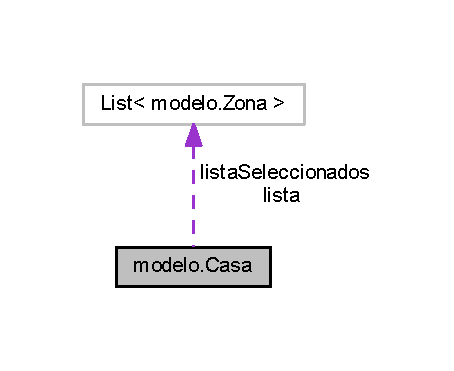
\includegraphics[width=218pt]{classmodelo_1_1_casa__coll__graph}
\end{center}
\end{figure}
\subsection*{Public Member Functions}
\begin{DoxyCompactItemize}
\item 
\mbox{\Hypertarget{classmodelo_1_1_casa_af9274bc27190d87445c1738f9521e1de}\label{classmodelo_1_1_casa_af9274bc27190d87445c1738f9521e1de}} 
List$<$ \mbox{\hyperlink{classmodelo_1_1_zona}{Zona}} $>$ {\bfseries cargar\+Datos\+Fichero} (String ruta\+Casa)
\item 
\mbox{\Hypertarget{classmodelo_1_1_casa_a504a6d0ee469d24256747979729793ae}\label{classmodelo_1_1_casa_a504a6d0ee469d24256747979729793ae}} 
void {\bfseries guardar\+Datos\+Fichero} (String ruta\+Casa)
\item 
\mbox{\Hypertarget{classmodelo_1_1_casa_acc00d762e914de9fb2226b936faa6628}\label{classmodelo_1_1_casa_acc00d762e914de9fb2226b936faa6628}} 
void {\bfseries add} (\mbox{\hyperlink{classmodelo_1_1_zona}{Zona}} zona)
\item 
\mbox{\Hypertarget{classmodelo_1_1_casa_adb043de5db6f7a315518085206568667}\label{classmodelo_1_1_casa_adb043de5db6f7a315518085206568667}} 
int {\bfseries get\+Next\+Value} (String tipo)
\item 
\mbox{\Hypertarget{classmodelo_1_1_casa_aa739909f439596b93dfbbd899f0ec740}\label{classmodelo_1_1_casa_aa739909f439596b93dfbbd899f0ec740}} 
void {\bfseries recargar\+Datos} (String ruta\+Casa)
\item 
\mbox{\Hypertarget{classmodelo_1_1_casa_acb5c7d204a097018d4fcb24b24b19537}\label{classmodelo_1_1_casa_acb5c7d204a097018d4fcb24b24b19537}} 
void {\bfseries remove} (\mbox{\hyperlink{classmodelo_1_1_zona}{Zona}} zona)
\item 
\mbox{\Hypertarget{classmodelo_1_1_casa_af00a9d3d107d6574ff06bff594c3971e}\label{classmodelo_1_1_casa_af00a9d3d107d6574ff06bff594c3971e}} 
void {\bfseries remove} (int indice)
\item 
\mbox{\Hypertarget{classmodelo_1_1_casa_a65e195399c3dac20e34b6201c666e97f}\label{classmodelo_1_1_casa_a65e195399c3dac20e34b6201c666e97f}} 
\mbox{\hyperlink{classmodelo_1_1_zona}{Zona}} \mbox{[}$\,$\mbox{]} {\bfseries get\+Strings\+By\+Type} (String type)
\item 
\mbox{\Hypertarget{classmodelo_1_1_casa_a2f915f8146b2bf9aac77bd76d40a7c3d}\label{classmodelo_1_1_casa_a2f915f8146b2bf9aac77bd76d40a7c3d}} 
List$<$ \mbox{\hyperlink{classmodelo_1_1_zona}{Zona}} $>$ {\bfseries get\+Seleccionados} ()
\item 
\mbox{\Hypertarget{classmodelo_1_1_casa_a82e53172ee38914af2b3edd24d65004f}\label{classmodelo_1_1_casa_a82e53172ee38914af2b3edd24d65004f}} 
Object {\bfseries get\+Element\+At} (int index)
\item 
\mbox{\Hypertarget{classmodelo_1_1_casa_a81cbd6dd883f5dc86616dc292d01efb7}\label{classmodelo_1_1_casa_a81cbd6dd883f5dc86616dc292d01efb7}} 
int {\bfseries get\+Size} ()
\item 
\mbox{\Hypertarget{classmodelo_1_1_casa_ae424bde8585ebf744728e2f6a79d9241}\label{classmodelo_1_1_casa_ae424bde8585ebf744728e2f6a79d9241}} 
List$<$ \mbox{\hyperlink{classmodelo_1_1_zona}{Zona}} $>$ {\bfseries get\+Copia\+Lista} ()
\item 
\mbox{\Hypertarget{classmodelo_1_1_casa_ae81948c050f1cc75212453a626f9e48f}\label{classmodelo_1_1_casa_ae81948c050f1cc75212453a626f9e48f}} 
int {\bfseries get\+Size\+By\+Type} (String type)
\item 
\mbox{\Hypertarget{classmodelo_1_1_casa_a50685b459f8c975d5305478b18526914}\label{classmodelo_1_1_casa_a50685b459f8c975d5305478b18526914}} 
String {\bfseries get\+Ruta\+Casa\+Config} ()
\item 
\mbox{\Hypertarget{classmodelo_1_1_casa_a453497c80f101aaf649b29c2dc301a6f}\label{classmodelo_1_1_casa_a453497c80f101aaf649b29c2dc301a6f}} 
void {\bfseries set\+Ruta\+Casa\+Config} (String ruta\+Casa\+Config)
\end{DoxyCompactItemize}


The documentation for this class was generated from the following file\+:\begin{DoxyCompactItemize}
\item 
C\+:/\+Users/\+Ander/\+Documents/\+Java/\+Dream\+Housev2/src/modelo/Casa.\+java\end{DoxyCompactItemize}

\hypertarget{classcontrolador_1_1_controlador_acciones_menu_config}{}\section{controlador.\+Controlador\+Acciones\+Menu\+Config Class Reference}
\label{classcontrolador_1_1_controlador_acciones_menu_config}\index{controlador.\+Controlador\+Acciones\+Menu\+Config@{controlador.\+Controlador\+Acciones\+Menu\+Config}}


Inheritance diagram for controlador.\+Controlador\+Acciones\+Menu\+Config\+:
\nopagebreak
\begin{figure}[H]
\begin{center}
\leavevmode
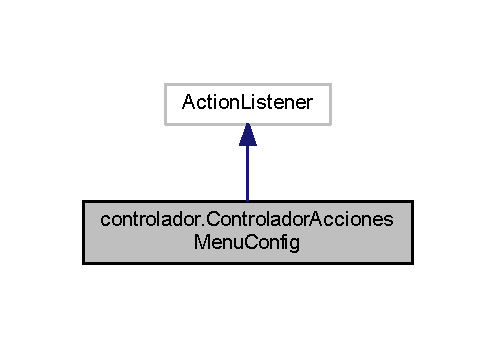
\includegraphics[width=238pt]{classcontrolador_1_1_controlador_acciones_menu_config__inherit__graph}
\end{center}
\end{figure}


Collaboration diagram for controlador.\+Controlador\+Acciones\+Menu\+Config\+:
\nopagebreak
\begin{figure}[H]
\begin{center}
\leavevmode
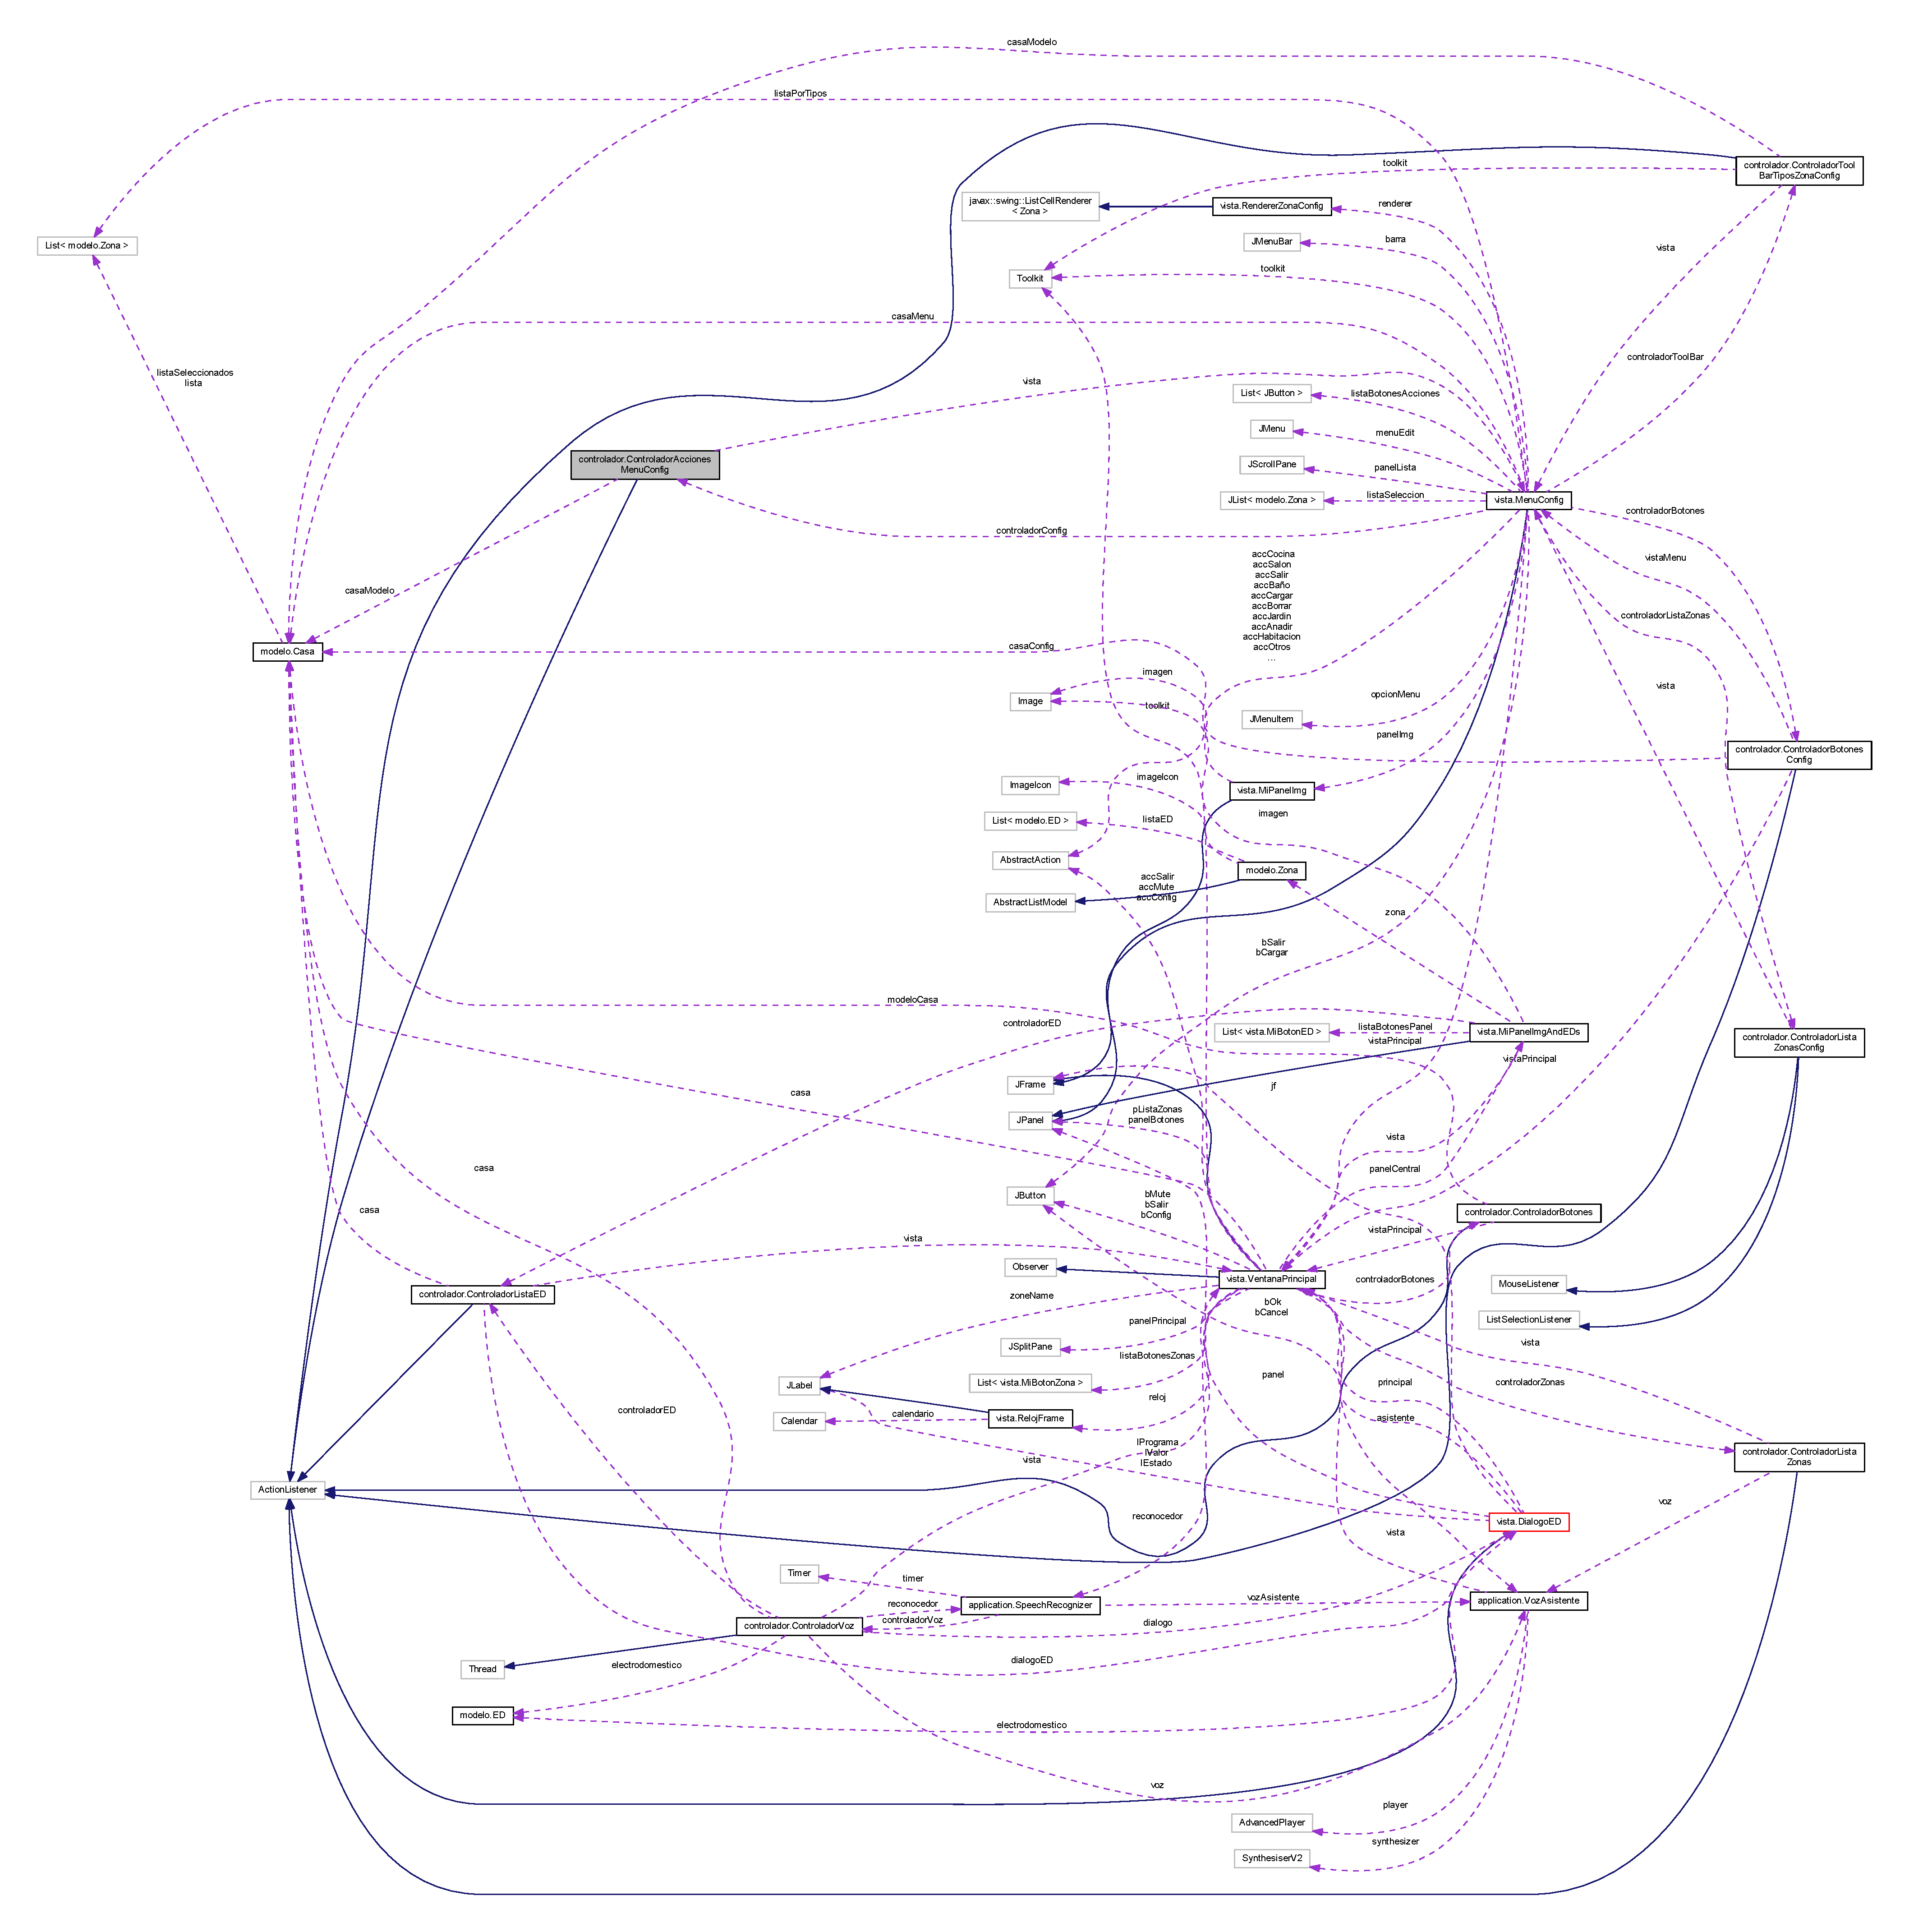
\includegraphics[width=350pt]{classcontrolador_1_1_controlador_acciones_menu_config__coll__graph}
\end{center}
\end{figure}
\subsection*{Public Member Functions}
\begin{DoxyCompactItemize}
\item 
\mbox{\Hypertarget{classcontrolador_1_1_controlador_acciones_menu_config_a4170bd70b4aec4fdb00586176b624ffe}\label{classcontrolador_1_1_controlador_acciones_menu_config_a4170bd70b4aec4fdb00586176b624ffe}} 
{\bfseries Controlador\+Acciones\+Menu\+Config} (\mbox{\hyperlink{classvista_1_1_menu_config}{Menu\+Config}} vista, \mbox{\hyperlink{classmodelo_1_1_casa}{Casa}} modelo)
\item 
\mbox{\Hypertarget{classcontrolador_1_1_controlador_acciones_menu_config_aa3e8635c243c1d61bea4ba8ef3a20f48}\label{classcontrolador_1_1_controlador_acciones_menu_config_aa3e8635c243c1d61bea4ba8ef3a20f48}} 
void {\bfseries action\+Performed} (Action\+Event e)
\end{DoxyCompactItemize}


The documentation for this class was generated from the following file\+:\begin{DoxyCompactItemize}
\item 
C\+:/\+Users/\+Ander/\+Documents/\+Java/\+Dream\+Housev2/src/controlador/Controlador\+Acciones\+Menu\+Config.\+java\end{DoxyCompactItemize}

\hypertarget{classcontrolador_1_1_controlador_a_xC3_xB1adir_editar_e_d}{}\section{controlador.\+Controlador\+Añadir\+Editar\+ED Class Reference}
\label{classcontrolador_1_1_controlador_a_xC3_xB1adir_editar_e_d}\index{controlador.\+Controlador\+Añadir\+Editar\+ED@{controlador.\+Controlador\+Añadir\+Editar\+ED}}


Inheritance diagram for controlador.\+Controlador\+Añadir\+Editar\+ED\+:
\nopagebreak
\begin{figure}[H]
\begin{center}
\leavevmode
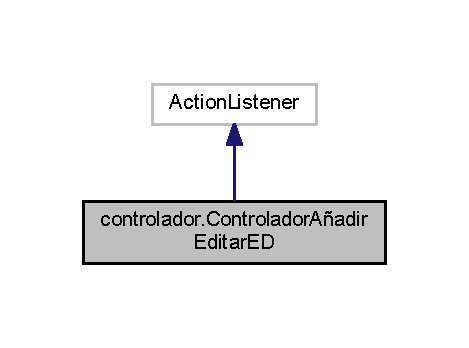
\includegraphics[width=225pt]{classcontrolador_1_1_controlador_a_xC3_xB1adir_editar_e_d__inherit__graph}
\end{center}
\end{figure}


Collaboration diagram for controlador.\+Controlador\+Añadir\+Editar\+ED\+:
\nopagebreak
\begin{figure}[H]
\begin{center}
\leavevmode
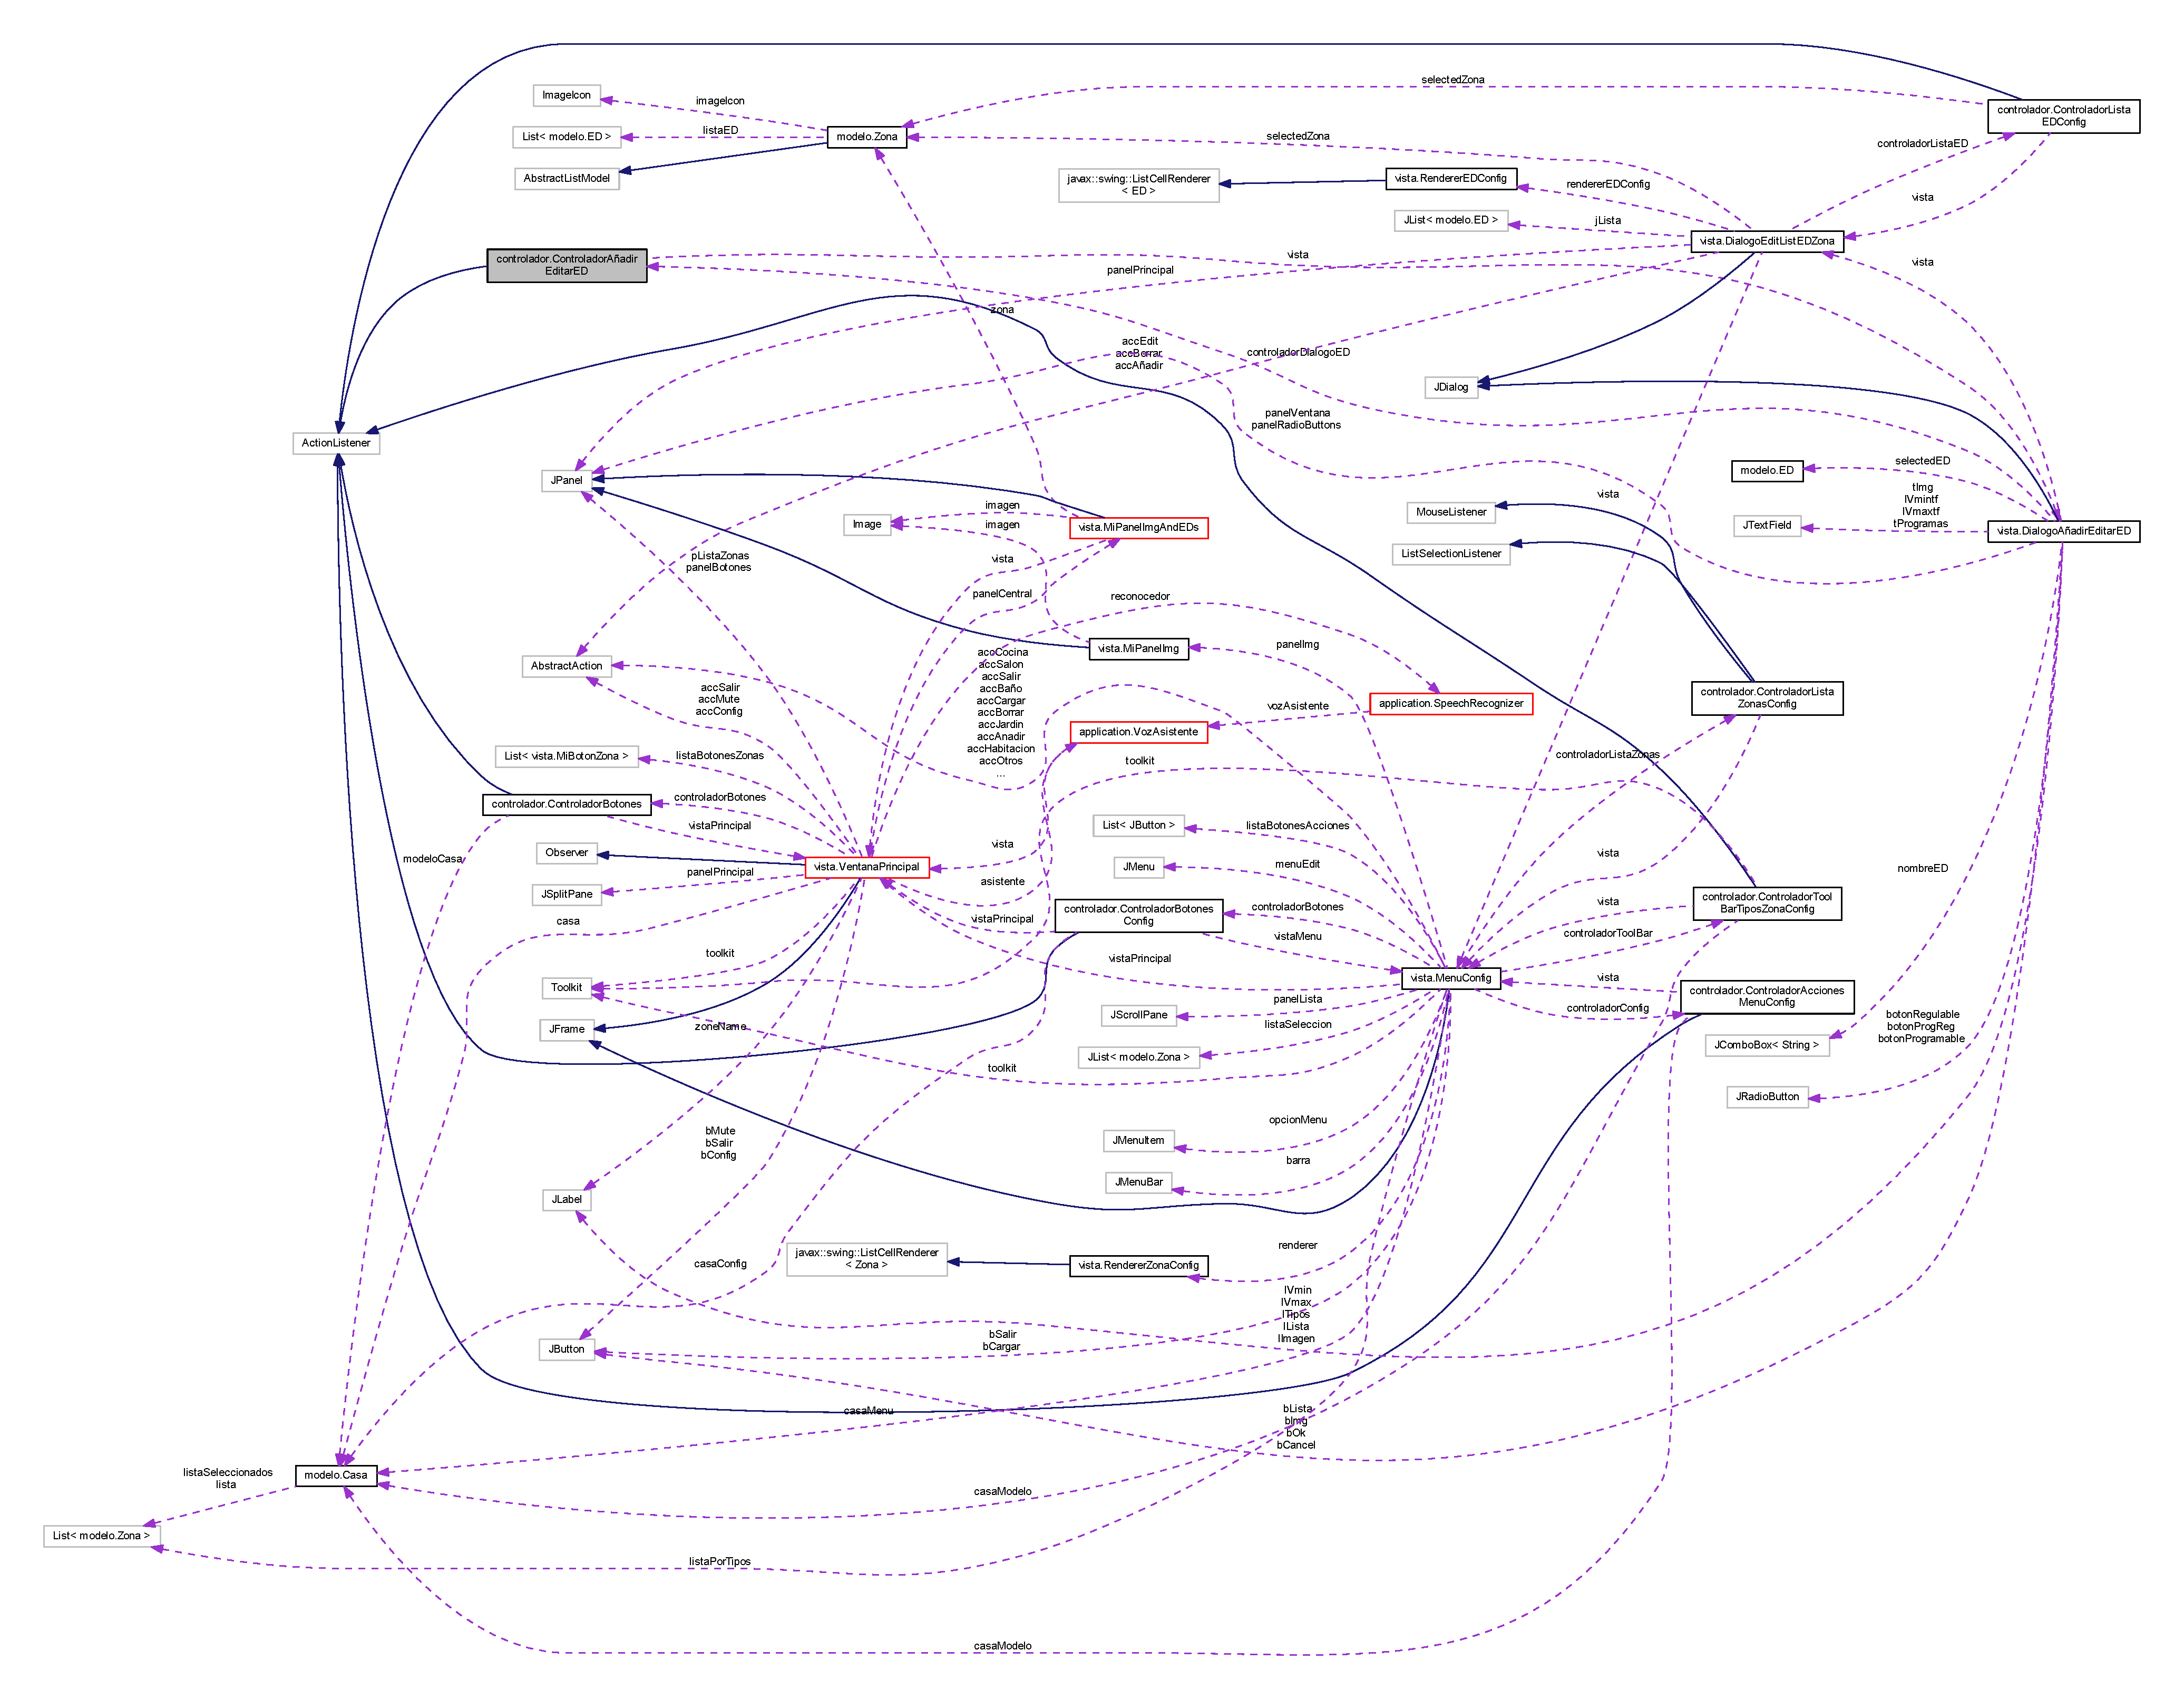
\includegraphics[width=350pt]{classcontrolador_1_1_controlador_a_xC3_xB1adir_editar_e_d__coll__graph}
\end{center}
\end{figure}
\subsection*{Public Member Functions}
\begin{DoxyCompactItemize}
\item 
\mbox{\Hypertarget{classcontrolador_1_1_controlador_a_xC3_xB1adir_editar_e_d_a0fa609c99f3c114987c35f821135d300}\label{classcontrolador_1_1_controlador_a_xC3_xB1adir_editar_e_d_a0fa609c99f3c114987c35f821135d300}} 
{\bfseries Controlador\+Añadir\+Editar\+ED} (\mbox{\hyperlink{classvista_1_1_dialogo_a_xC3_xB1adir_editar_e_d}{Dialogo\+Añadir\+Editar\+ED}} vista)
\item 
\mbox{\Hypertarget{classcontrolador_1_1_controlador_a_xC3_xB1adir_editar_e_d_a3fd00d9c11231733a48c13b71fd304a6}\label{classcontrolador_1_1_controlador_a_xC3_xB1adir_editar_e_d_a3fd00d9c11231733a48c13b71fd304a6}} 
void {\bfseries action\+Performed} (Action\+Event e)
\end{DoxyCompactItemize}


The documentation for this class was generated from the following file\+:\begin{DoxyCompactItemize}
\item 
C\+:/\+Users/\+Ander/\+Documents/\+Java/\+Dream\+Housev2/src/controlador/Controlador\+Añadir\+Editar\+E\+D.\+java\end{DoxyCompactItemize}

\hypertarget{classcontrolador_1_1_controlador_a_xC3_xB1adir_editar_zona}{}\section{controlador.\+Controlador\+Añadir\+Editar\+Zona Class Reference}
\label{classcontrolador_1_1_controlador_a_xC3_xB1adir_editar_zona}\index{controlador.\+Controlador\+Añadir\+Editar\+Zona@{controlador.\+Controlador\+Añadir\+Editar\+Zona}}


Inheritance diagram for controlador.\+Controlador\+Añadir\+Editar\+Zona\+:
\nopagebreak
\begin{figure}[H]
\begin{center}
\leavevmode
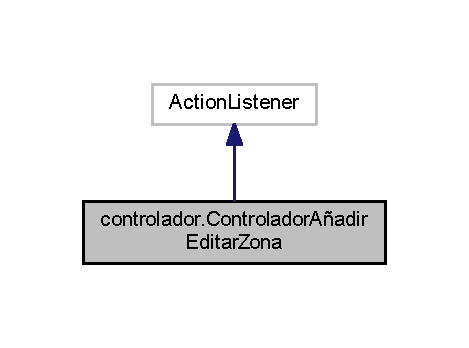
\includegraphics[width=225pt]{classcontrolador_1_1_controlador_a_xC3_xB1adir_editar_zona__inherit__graph}
\end{center}
\end{figure}


Collaboration diagram for controlador.\+Controlador\+Añadir\+Editar\+Zona\+:
\nopagebreak
\begin{figure}[H]
\begin{center}
\leavevmode
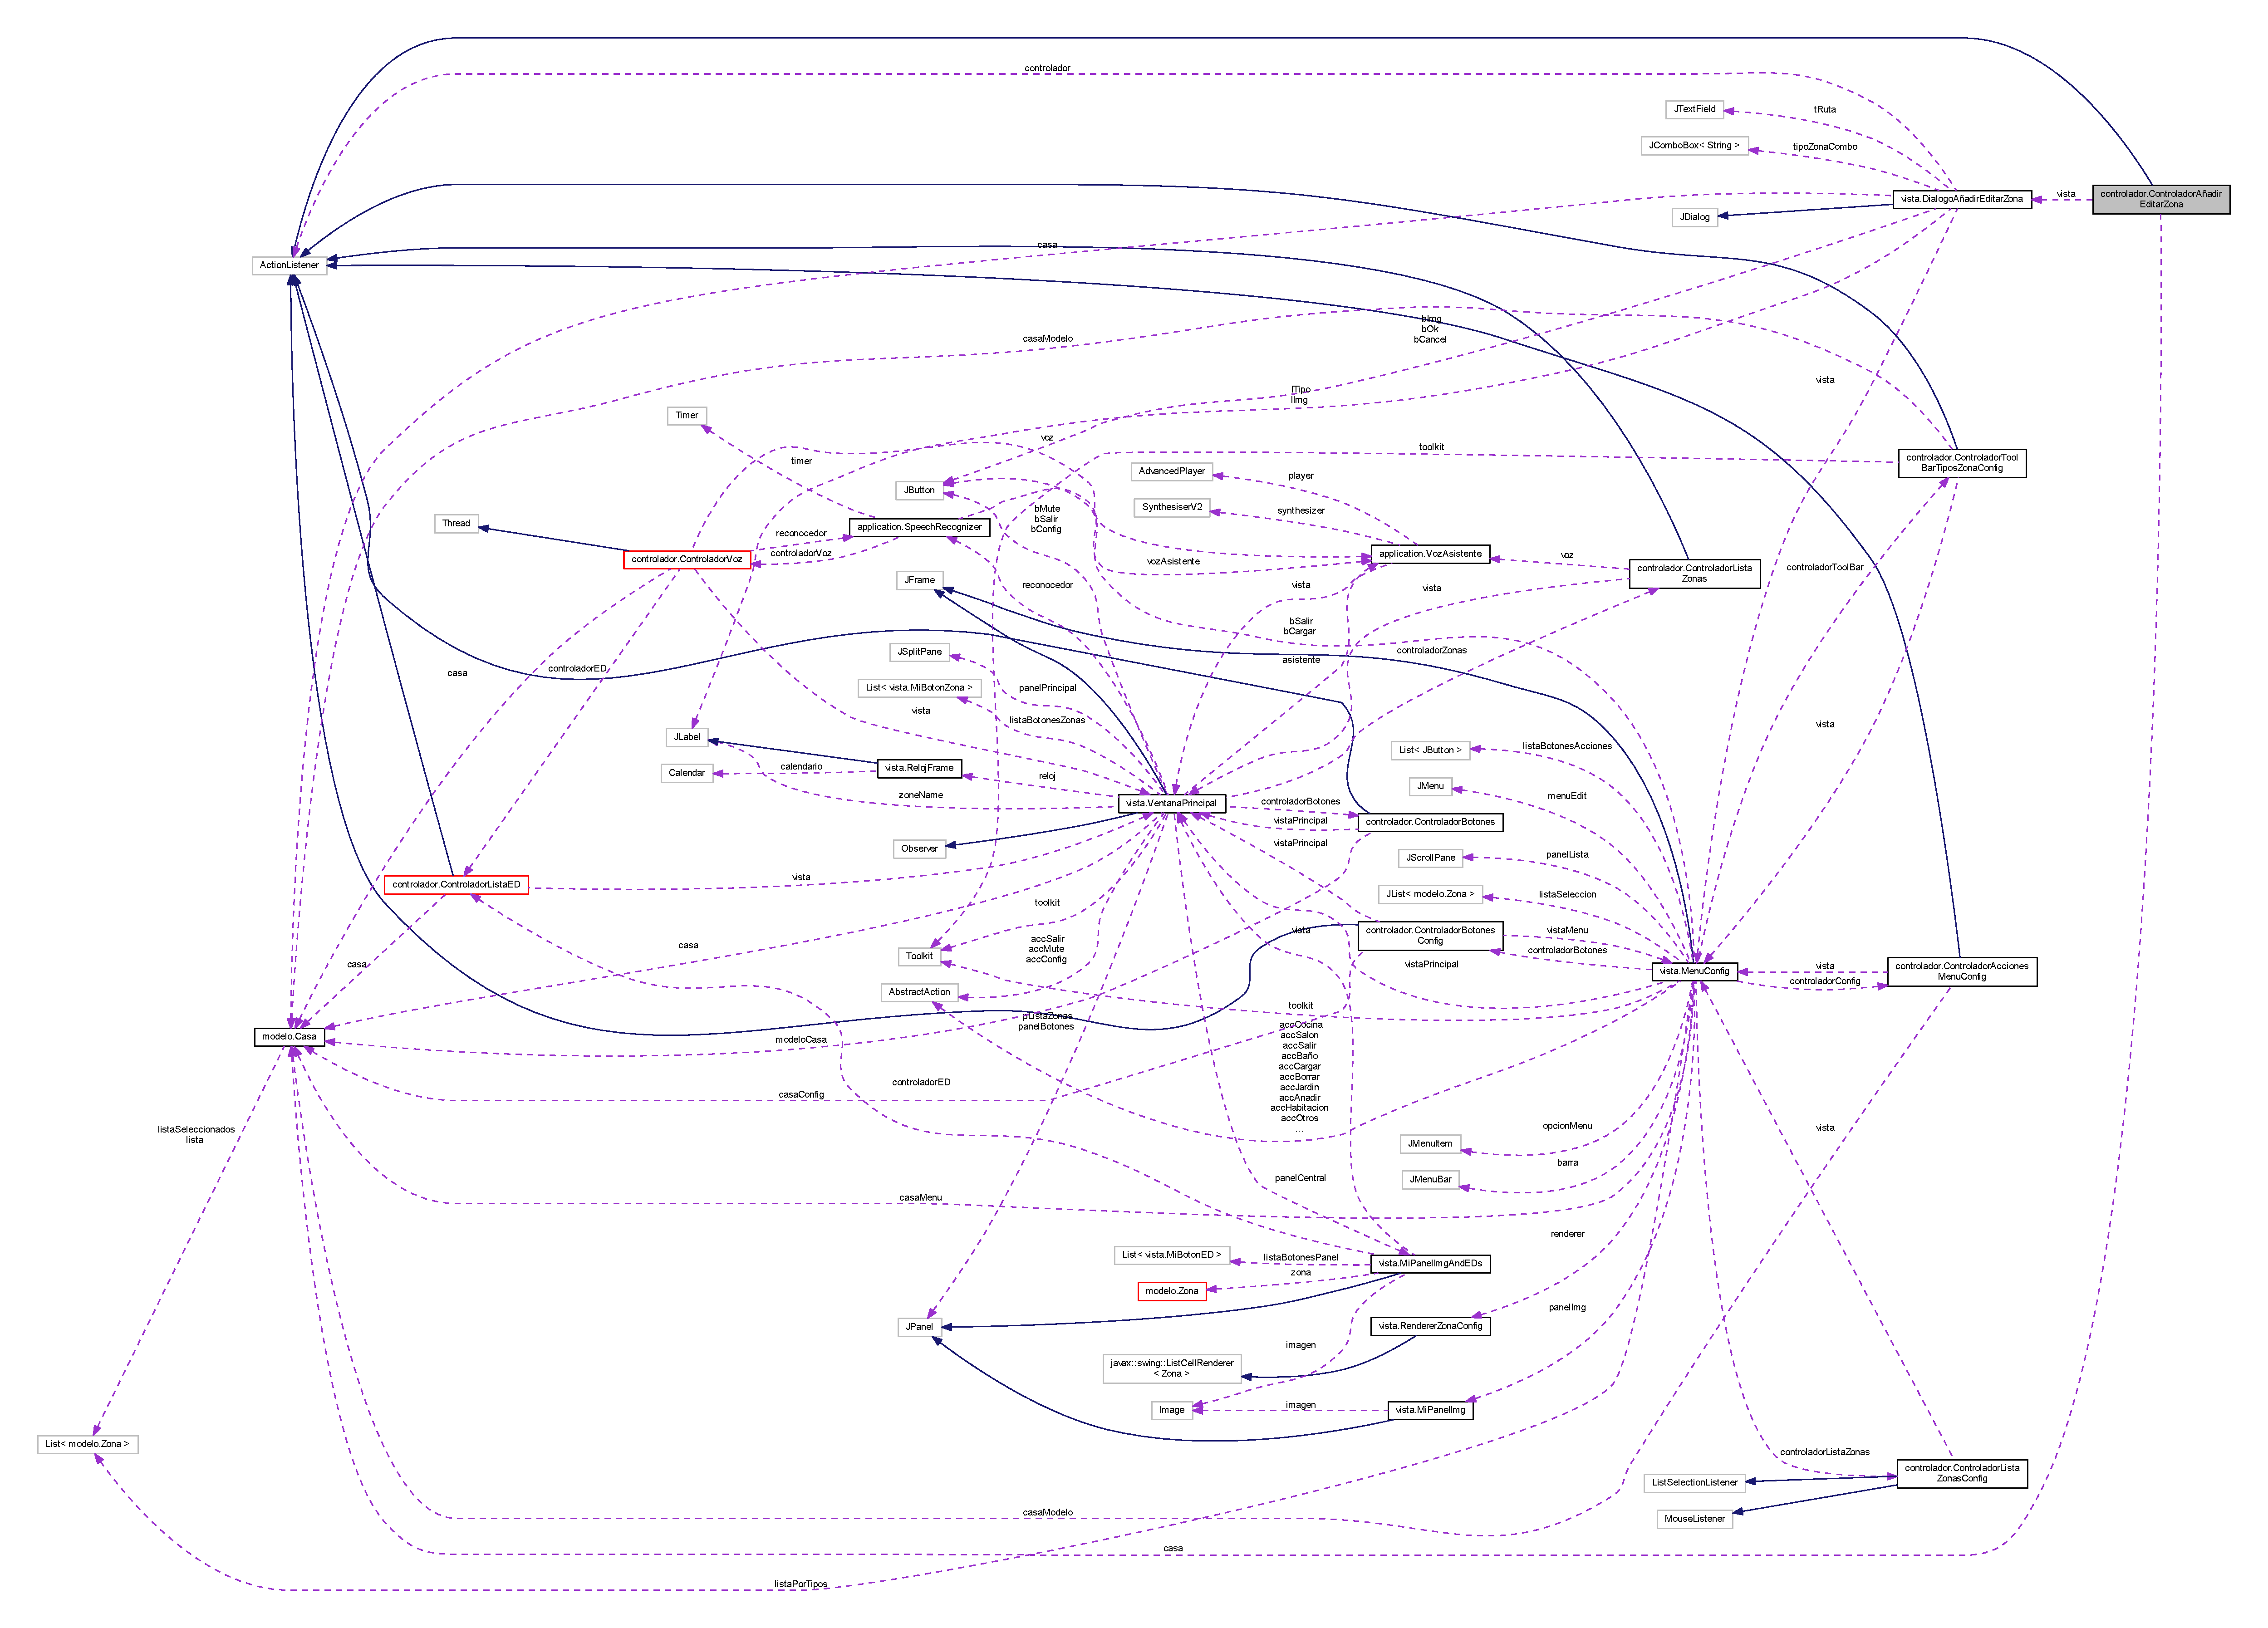
\includegraphics[width=350pt]{classcontrolador_1_1_controlador_a_xC3_xB1adir_editar_zona__coll__graph}
\end{center}
\end{figure}
\subsection*{Public Member Functions}
\begin{DoxyCompactItemize}
\item 
\mbox{\Hypertarget{classcontrolador_1_1_controlador_a_xC3_xB1adir_editar_zona_a2a27c449b5c5bdd3a6f1cf05d600bd97}\label{classcontrolador_1_1_controlador_a_xC3_xB1adir_editar_zona_a2a27c449b5c5bdd3a6f1cf05d600bd97}} 
{\bfseries Controlador\+Añadir\+Editar\+Zona} (\mbox{\hyperlink{classvista_1_1_dialogo_a_xC3_xB1adir_editar_zona}{Dialogo\+Añadir\+Editar\+Zona}} vista, \mbox{\hyperlink{classmodelo_1_1_casa}{Casa}} casa, boolean esta\+Añadiendo)
\item 
\mbox{\Hypertarget{classcontrolador_1_1_controlador_a_xC3_xB1adir_editar_zona_adc1d0f47740fb96ef70428061228efd1}\label{classcontrolador_1_1_controlador_a_xC3_xB1adir_editar_zona_adc1d0f47740fb96ef70428061228efd1}} 
void {\bfseries action\+Performed} (Action\+Event e)
\end{DoxyCompactItemize}


The documentation for this class was generated from the following file\+:\begin{DoxyCompactItemize}
\item 
C\+:/\+Users/\+Ander/\+Documents/\+Java/\+Dream\+Housev2/src/controlador/Controlador\+Añadir\+Editar\+Zona.\+java\end{DoxyCompactItemize}

\hypertarget{classcontrolador_1_1_controlador_botones}{}\section{controlador.\+Controlador\+Botones Class Reference}
\label{classcontrolador_1_1_controlador_botones}\index{controlador.\+Controlador\+Botones@{controlador.\+Controlador\+Botones}}


Inheritance diagram for controlador.\+Controlador\+Botones\+:
\nopagebreak
\begin{figure}[H]
\begin{center}
\leavevmode
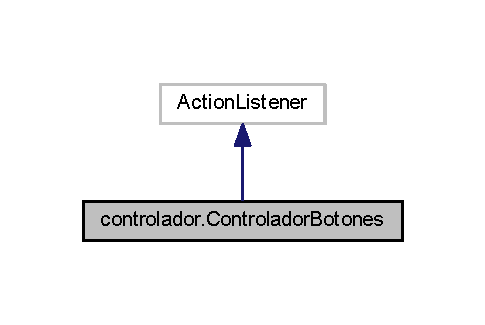
\includegraphics[width=233pt]{classcontrolador_1_1_controlador_botones__inherit__graph}
\end{center}
\end{figure}


Collaboration diagram for controlador.\+Controlador\+Botones\+:
\nopagebreak
\begin{figure}[H]
\begin{center}
\leavevmode
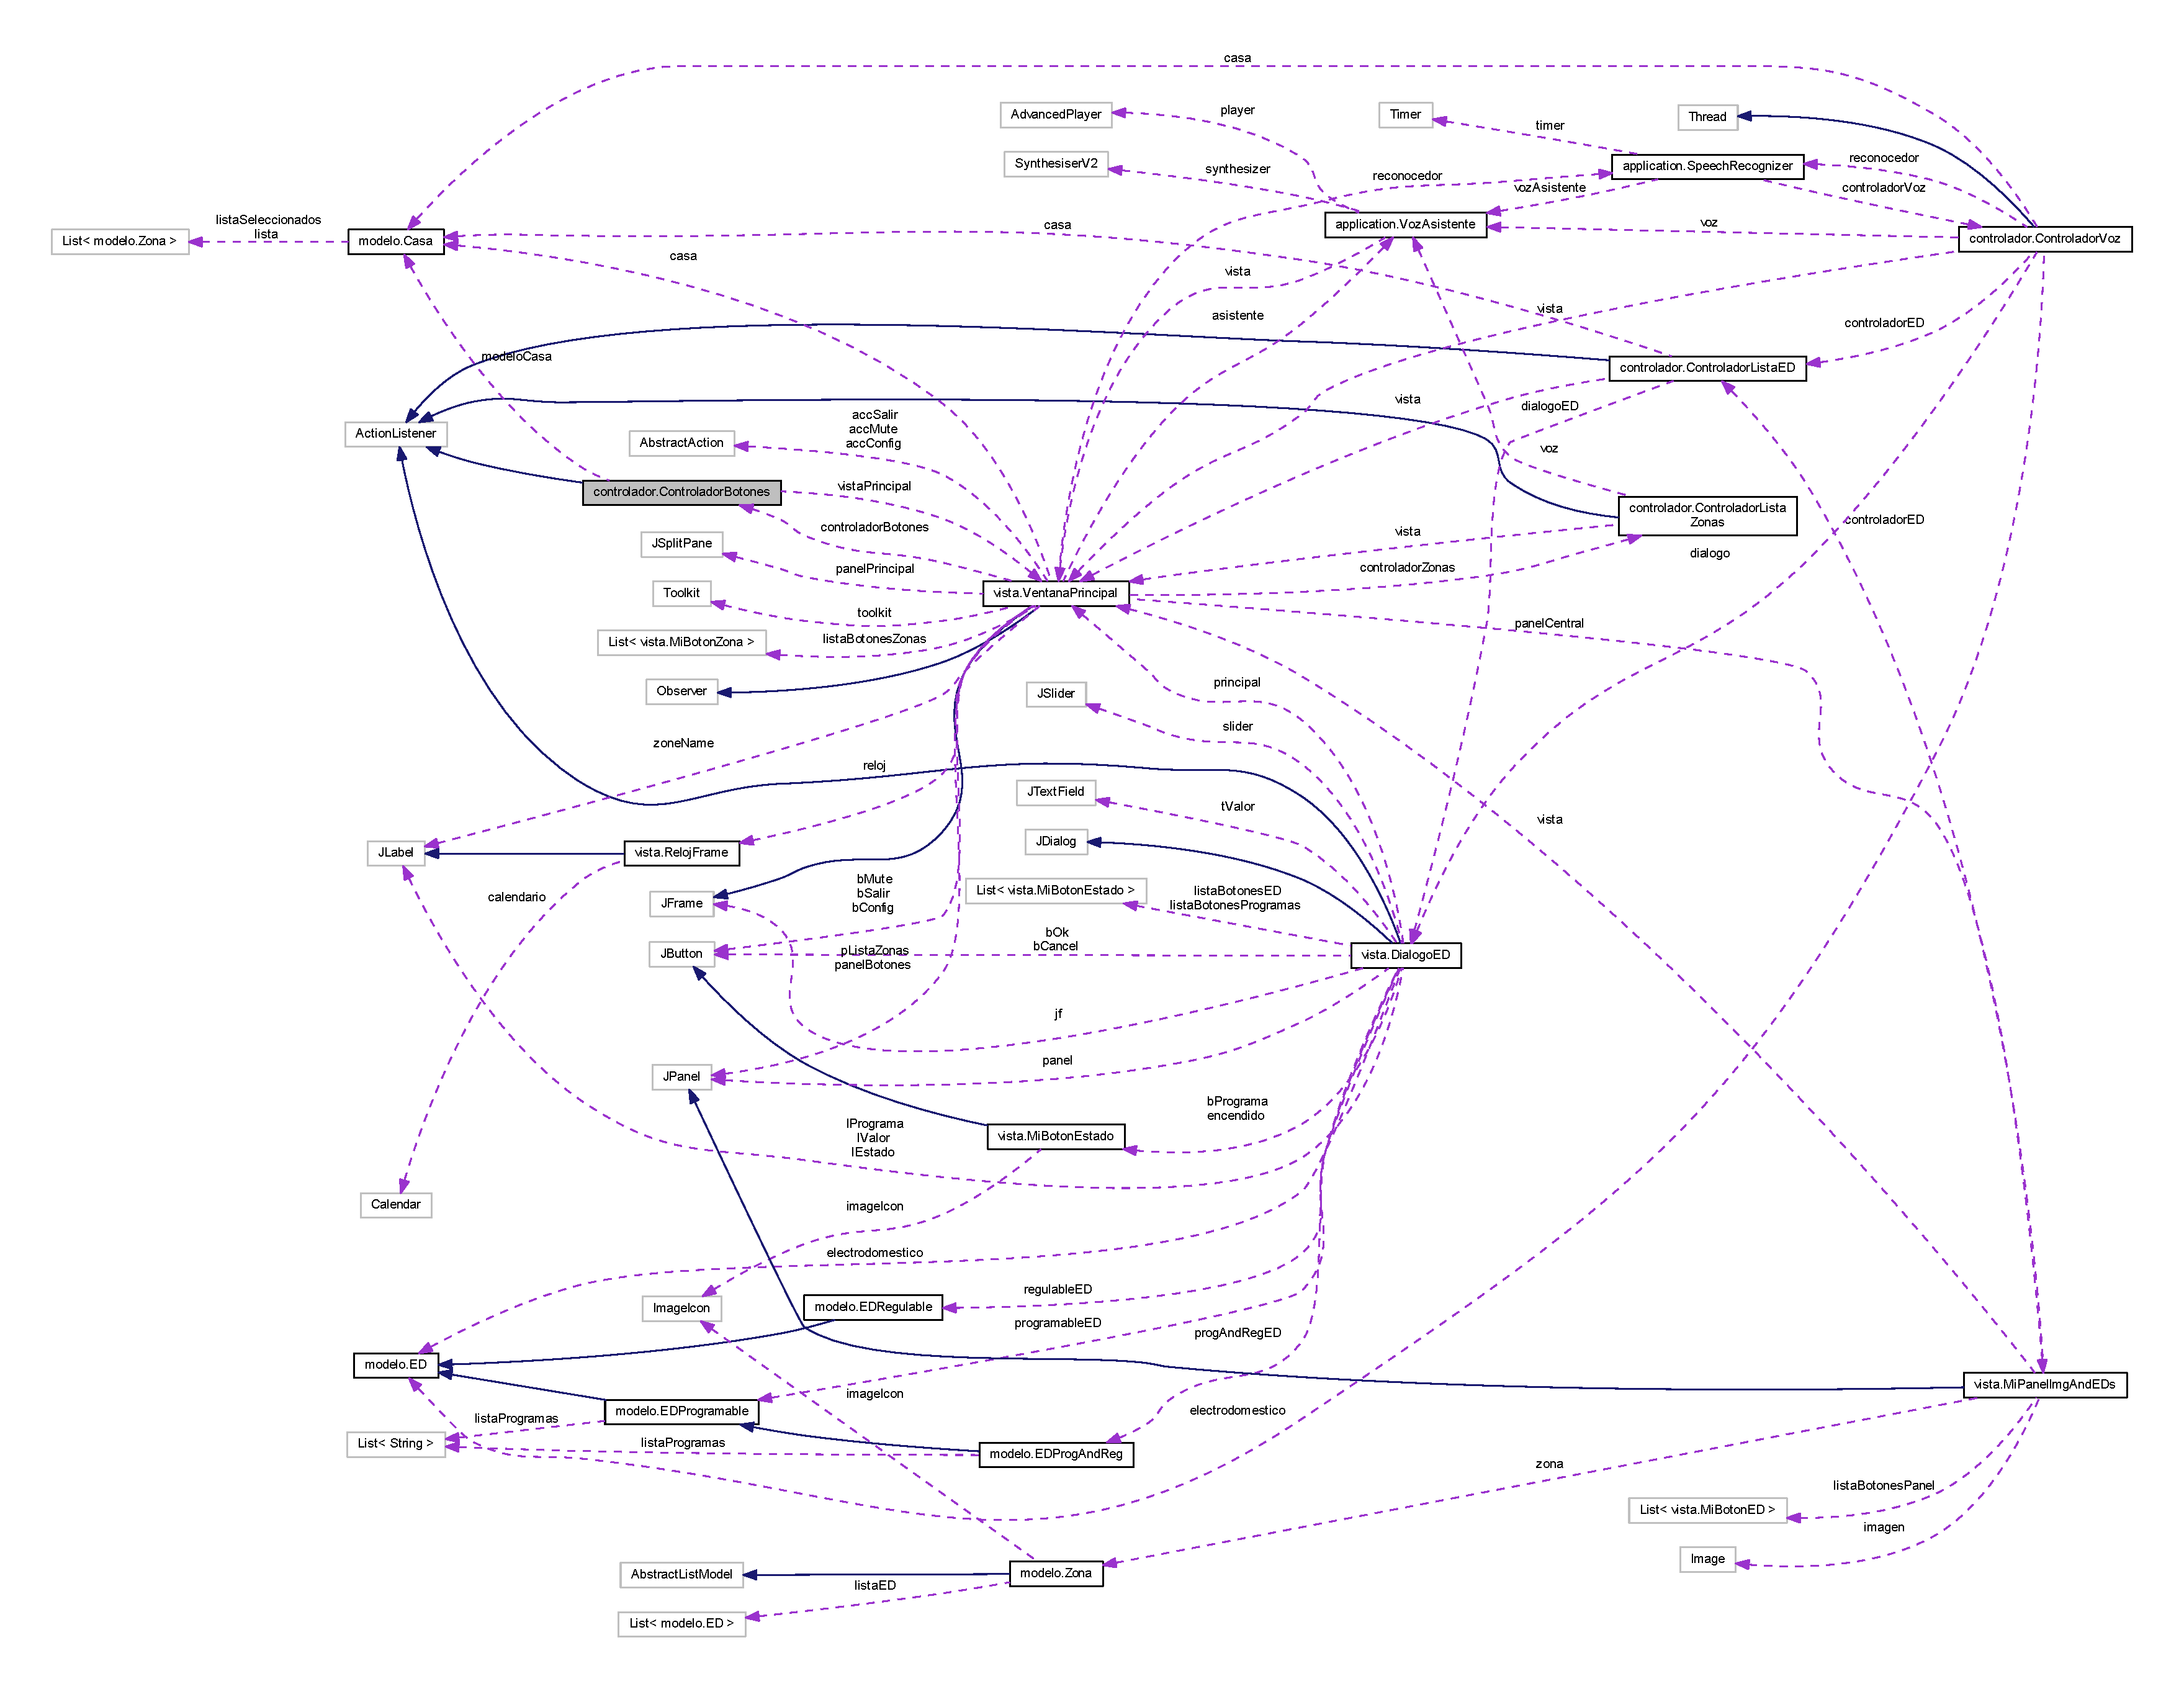
\includegraphics[width=350pt]{classcontrolador_1_1_controlador_botones__coll__graph}
\end{center}
\end{figure}
\subsection*{Public Member Functions}
\begin{DoxyCompactItemize}
\item 
\mbox{\Hypertarget{classcontrolador_1_1_controlador_botones_ad14c7f5b59b1e67e9af9019f7e309432}\label{classcontrolador_1_1_controlador_botones_ad14c7f5b59b1e67e9af9019f7e309432}} 
{\bfseries Controlador\+Botones} (\mbox{\hyperlink{classvista_1_1_ventana_principal}{Ventana\+Principal}} vista\+Principal, \mbox{\hyperlink{classmodelo_1_1_casa}{Casa}} modelo)
\item 
\mbox{\Hypertarget{classcontrolador_1_1_controlador_botones_a73a3073a9dd8e1d62ba20831005ecb48}\label{classcontrolador_1_1_controlador_botones_a73a3073a9dd8e1d62ba20831005ecb48}} 
void {\bfseries action\+Performed} (Action\+Event e)
\end{DoxyCompactItemize}


The documentation for this class was generated from the following file\+:\begin{DoxyCompactItemize}
\item 
C\+:/\+Users/\+Ander/\+Documents/\+Java/\+Dream\+Housev2/src/controlador/Controlador\+Botones.\+java\end{DoxyCompactItemize}

\hypertarget{classcontrolador_1_1_controlador_botones_config}{}\section{controlador.\+Controlador\+Botones\+Config Class Reference}
\label{classcontrolador_1_1_controlador_botones_config}\index{controlador.\+Controlador\+Botones\+Config@{controlador.\+Controlador\+Botones\+Config}}


Inheritance diagram for controlador.\+Controlador\+Botones\+Config\+:
\nopagebreak
\begin{figure}[H]
\begin{center}
\leavevmode
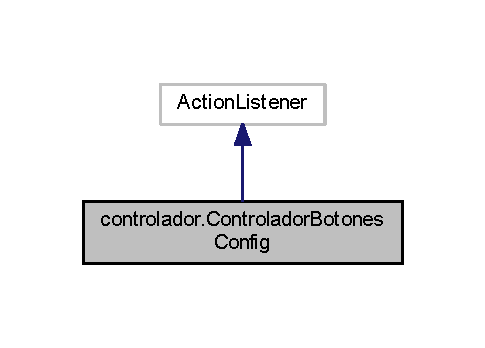
\includegraphics[width=233pt]{classcontrolador_1_1_controlador_botones_config__inherit__graph}
\end{center}
\end{figure}


Collaboration diagram for controlador.\+Controlador\+Botones\+Config\+:
\nopagebreak
\begin{figure}[H]
\begin{center}
\leavevmode
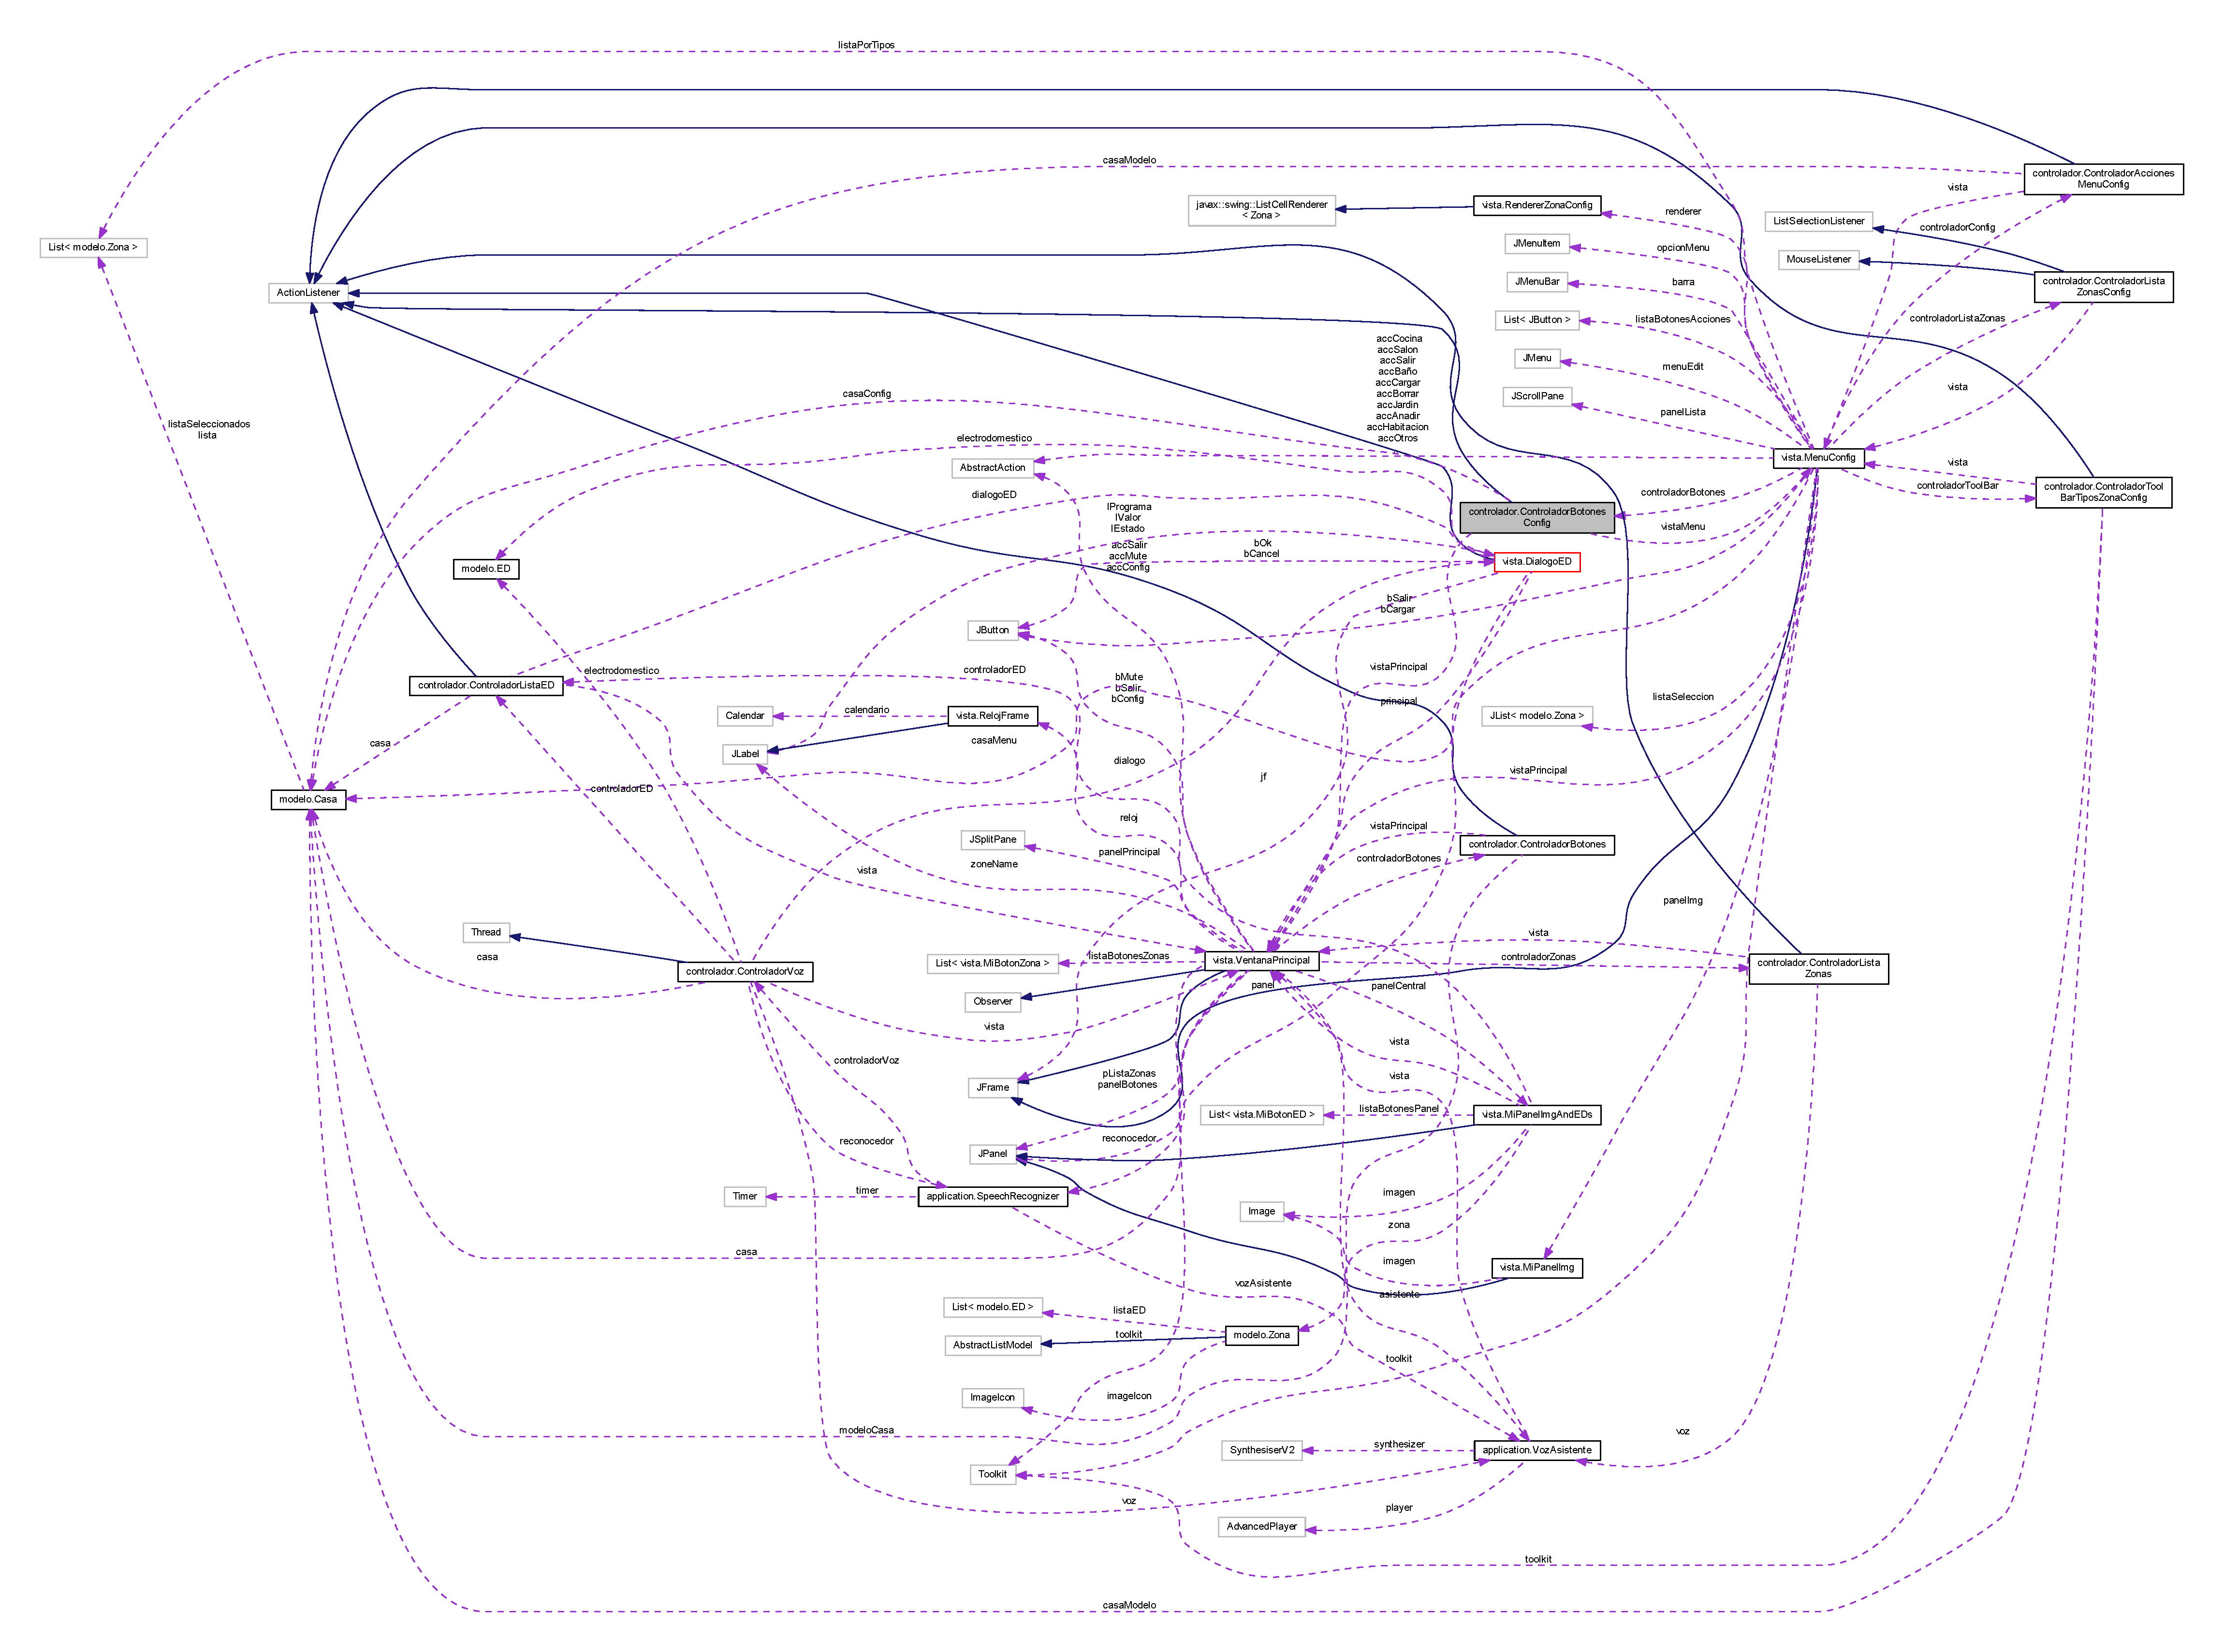
\includegraphics[width=350pt]{classcontrolador_1_1_controlador_botones_config__coll__graph}
\end{center}
\end{figure}
\subsection*{Public Member Functions}
\begin{DoxyCompactItemize}
\item 
\mbox{\Hypertarget{classcontrolador_1_1_controlador_botones_config_a4af8c80c8585506639754cfb7f77eb61}\label{classcontrolador_1_1_controlador_botones_config_a4af8c80c8585506639754cfb7f77eb61}} 
{\bfseries Controlador\+Botones\+Config} (\mbox{\hyperlink{classvista_1_1_menu_config}{Menu\+Config}} vista\+Menu, \mbox{\hyperlink{classmodelo_1_1_casa}{Casa}} casa\+Config, \mbox{\hyperlink{classvista_1_1_ventana_principal}{Ventana\+Principal}} vista\+Principal)
\item 
\mbox{\Hypertarget{classcontrolador_1_1_controlador_botones_config_a2cd5a386f11405de4564bc37e1f21850}\label{classcontrolador_1_1_controlador_botones_config_a2cd5a386f11405de4564bc37e1f21850}} 
void {\bfseries action\+Performed} (Action\+Event e)
\end{DoxyCompactItemize}


The documentation for this class was generated from the following file\+:\begin{DoxyCompactItemize}
\item 
C\+:/\+Users/\+Ander/\+Documents/\+Java/\+Dream\+Housev2/src/controlador/Controlador\+Botones\+Config.\+java\end{DoxyCompactItemize}

\hypertarget{classcontrolador_1_1_controlador_lista_e_d}{}\section{controlador.\+Controlador\+Lista\+ED Class Reference}
\label{classcontrolador_1_1_controlador_lista_e_d}\index{controlador.\+Controlador\+Lista\+ED@{controlador.\+Controlador\+Lista\+ED}}


Inheritance diagram for controlador.\+Controlador\+Lista\+ED\+:
\nopagebreak
\begin{figure}[H]
\begin{center}
\leavevmode
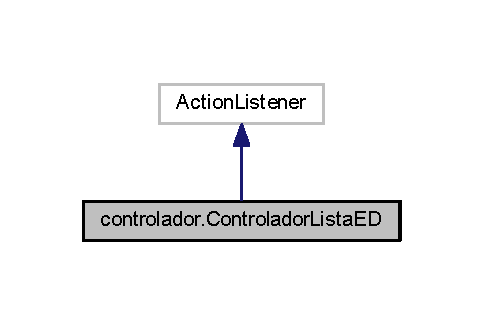
\includegraphics[width=232pt]{classcontrolador_1_1_controlador_lista_e_d__inherit__graph}
\end{center}
\end{figure}


Collaboration diagram for controlador.\+Controlador\+Lista\+ED\+:
\nopagebreak
\begin{figure}[H]
\begin{center}
\leavevmode
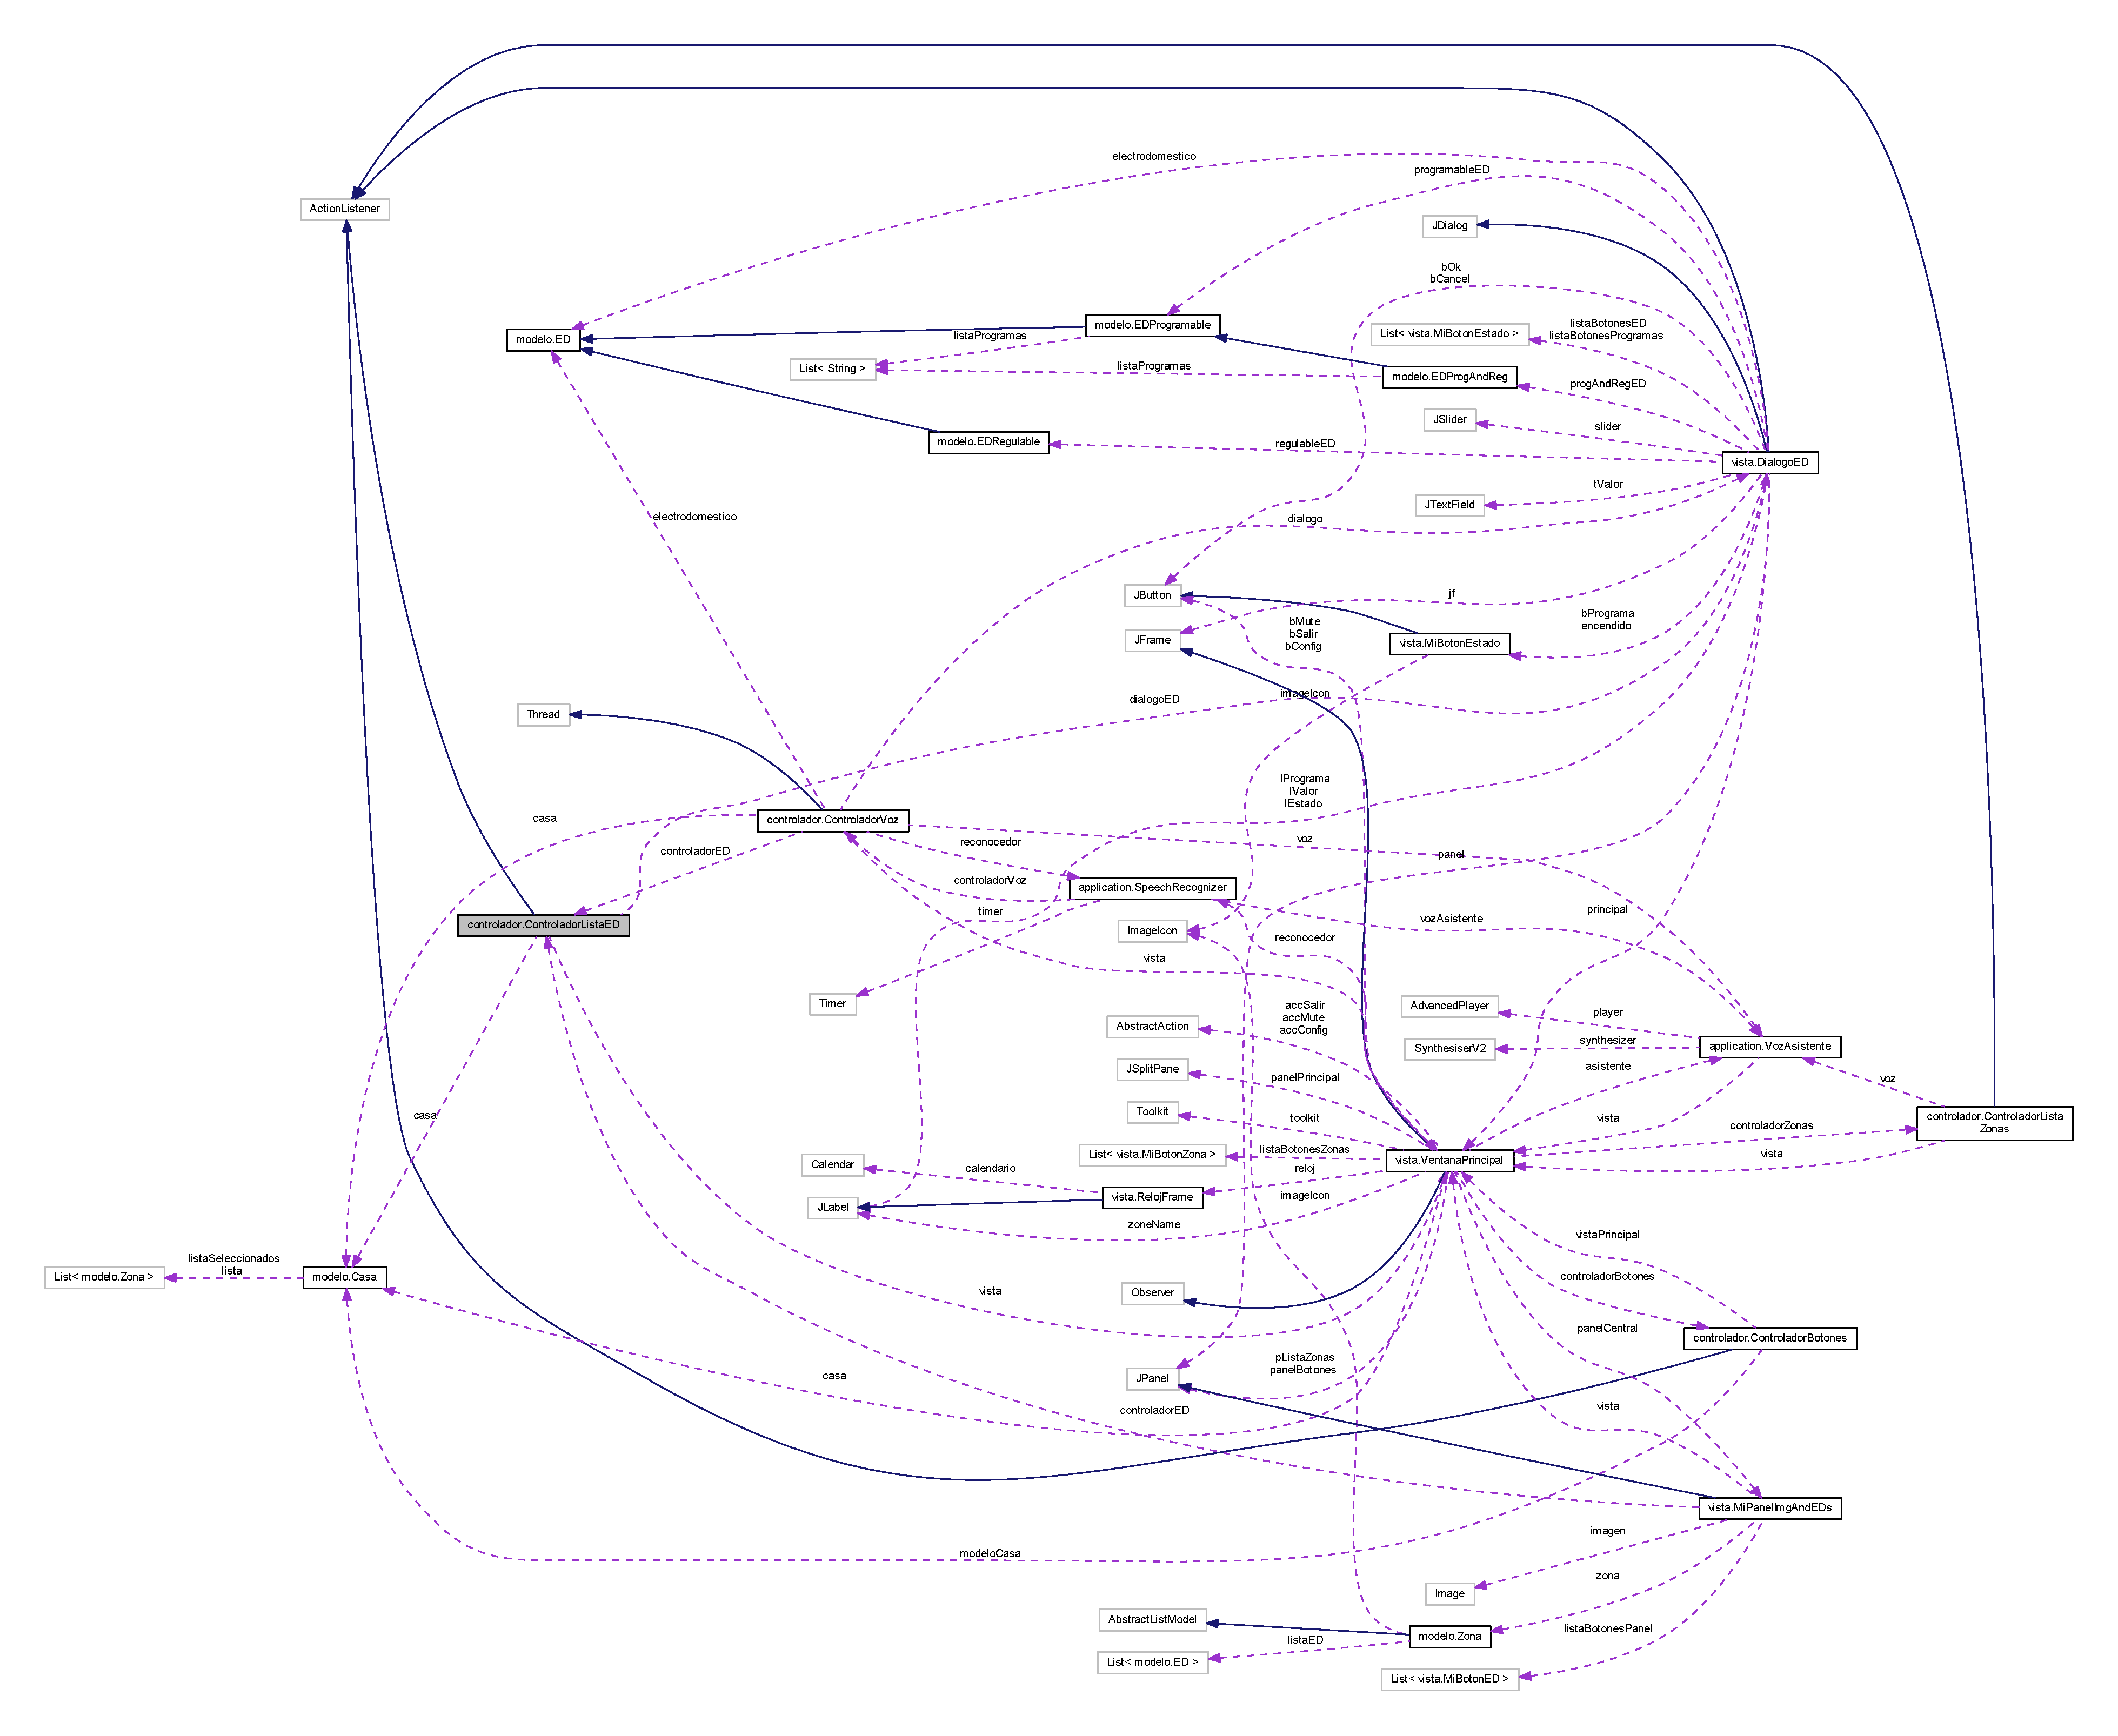
\includegraphics[width=350pt]{classcontrolador_1_1_controlador_lista_e_d__coll__graph}
\end{center}
\end{figure}
\subsection*{Public Member Functions}
\begin{DoxyCompactItemize}
\item 
\mbox{\Hypertarget{classcontrolador_1_1_controlador_lista_e_d_a104b9506109ea05b3d00ffc16041c97d}\label{classcontrolador_1_1_controlador_lista_e_d_a104b9506109ea05b3d00ffc16041c97d}} 
{\bfseries Controlador\+Lista\+ED} (\mbox{\hyperlink{classvista_1_1_ventana_principal}{Ventana\+Principal}} vista, \mbox{\hyperlink{classmodelo_1_1_casa}{Casa}} casa)
\item 
\mbox{\Hypertarget{classcontrolador_1_1_controlador_lista_e_d_a314311c80165a8dbc22415253dbecf16}\label{classcontrolador_1_1_controlador_lista_e_d_a314311c80165a8dbc22415253dbecf16}} 
void {\bfseries action\+Performed} (Action\+Event e)
\item 
\mbox{\Hypertarget{classcontrolador_1_1_controlador_lista_e_d_a3632ab1b0937e0e120ffddbbb453c02d}\label{classcontrolador_1_1_controlador_lista_e_d_a3632ab1b0937e0e120ffddbbb453c02d}} 
\mbox{\hyperlink{classvista_1_1_dialogo_e_d}{Dialogo\+ED}} {\bfseries get\+Dialogo\+ED} ()
\end{DoxyCompactItemize}


The documentation for this class was generated from the following file\+:\begin{DoxyCompactItemize}
\item 
C\+:/\+Users/\+Ander/\+Documents/\+Java/\+Dream\+Housev2/src/controlador/Controlador\+Lista\+E\+D.\+java\end{DoxyCompactItemize}

\hypertarget{classcontrolador_1_1_controlador_lista_e_d_config}{}\section{controlador.\+Controlador\+Lista\+E\+D\+Config Class Reference}
\label{classcontrolador_1_1_controlador_lista_e_d_config}\index{controlador.\+Controlador\+Lista\+E\+D\+Config@{controlador.\+Controlador\+Lista\+E\+D\+Config}}


Inheritance diagram for controlador.\+Controlador\+Lista\+E\+D\+Config\+:
\nopagebreak
\begin{figure}[H]
\begin{center}
\leavevmode
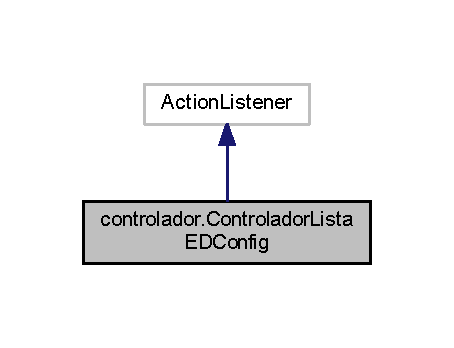
\includegraphics[width=218pt]{classcontrolador_1_1_controlador_lista_e_d_config__inherit__graph}
\end{center}
\end{figure}


Collaboration diagram for controlador.\+Controlador\+Lista\+E\+D\+Config\+:
\nopagebreak
\begin{figure}[H]
\begin{center}
\leavevmode
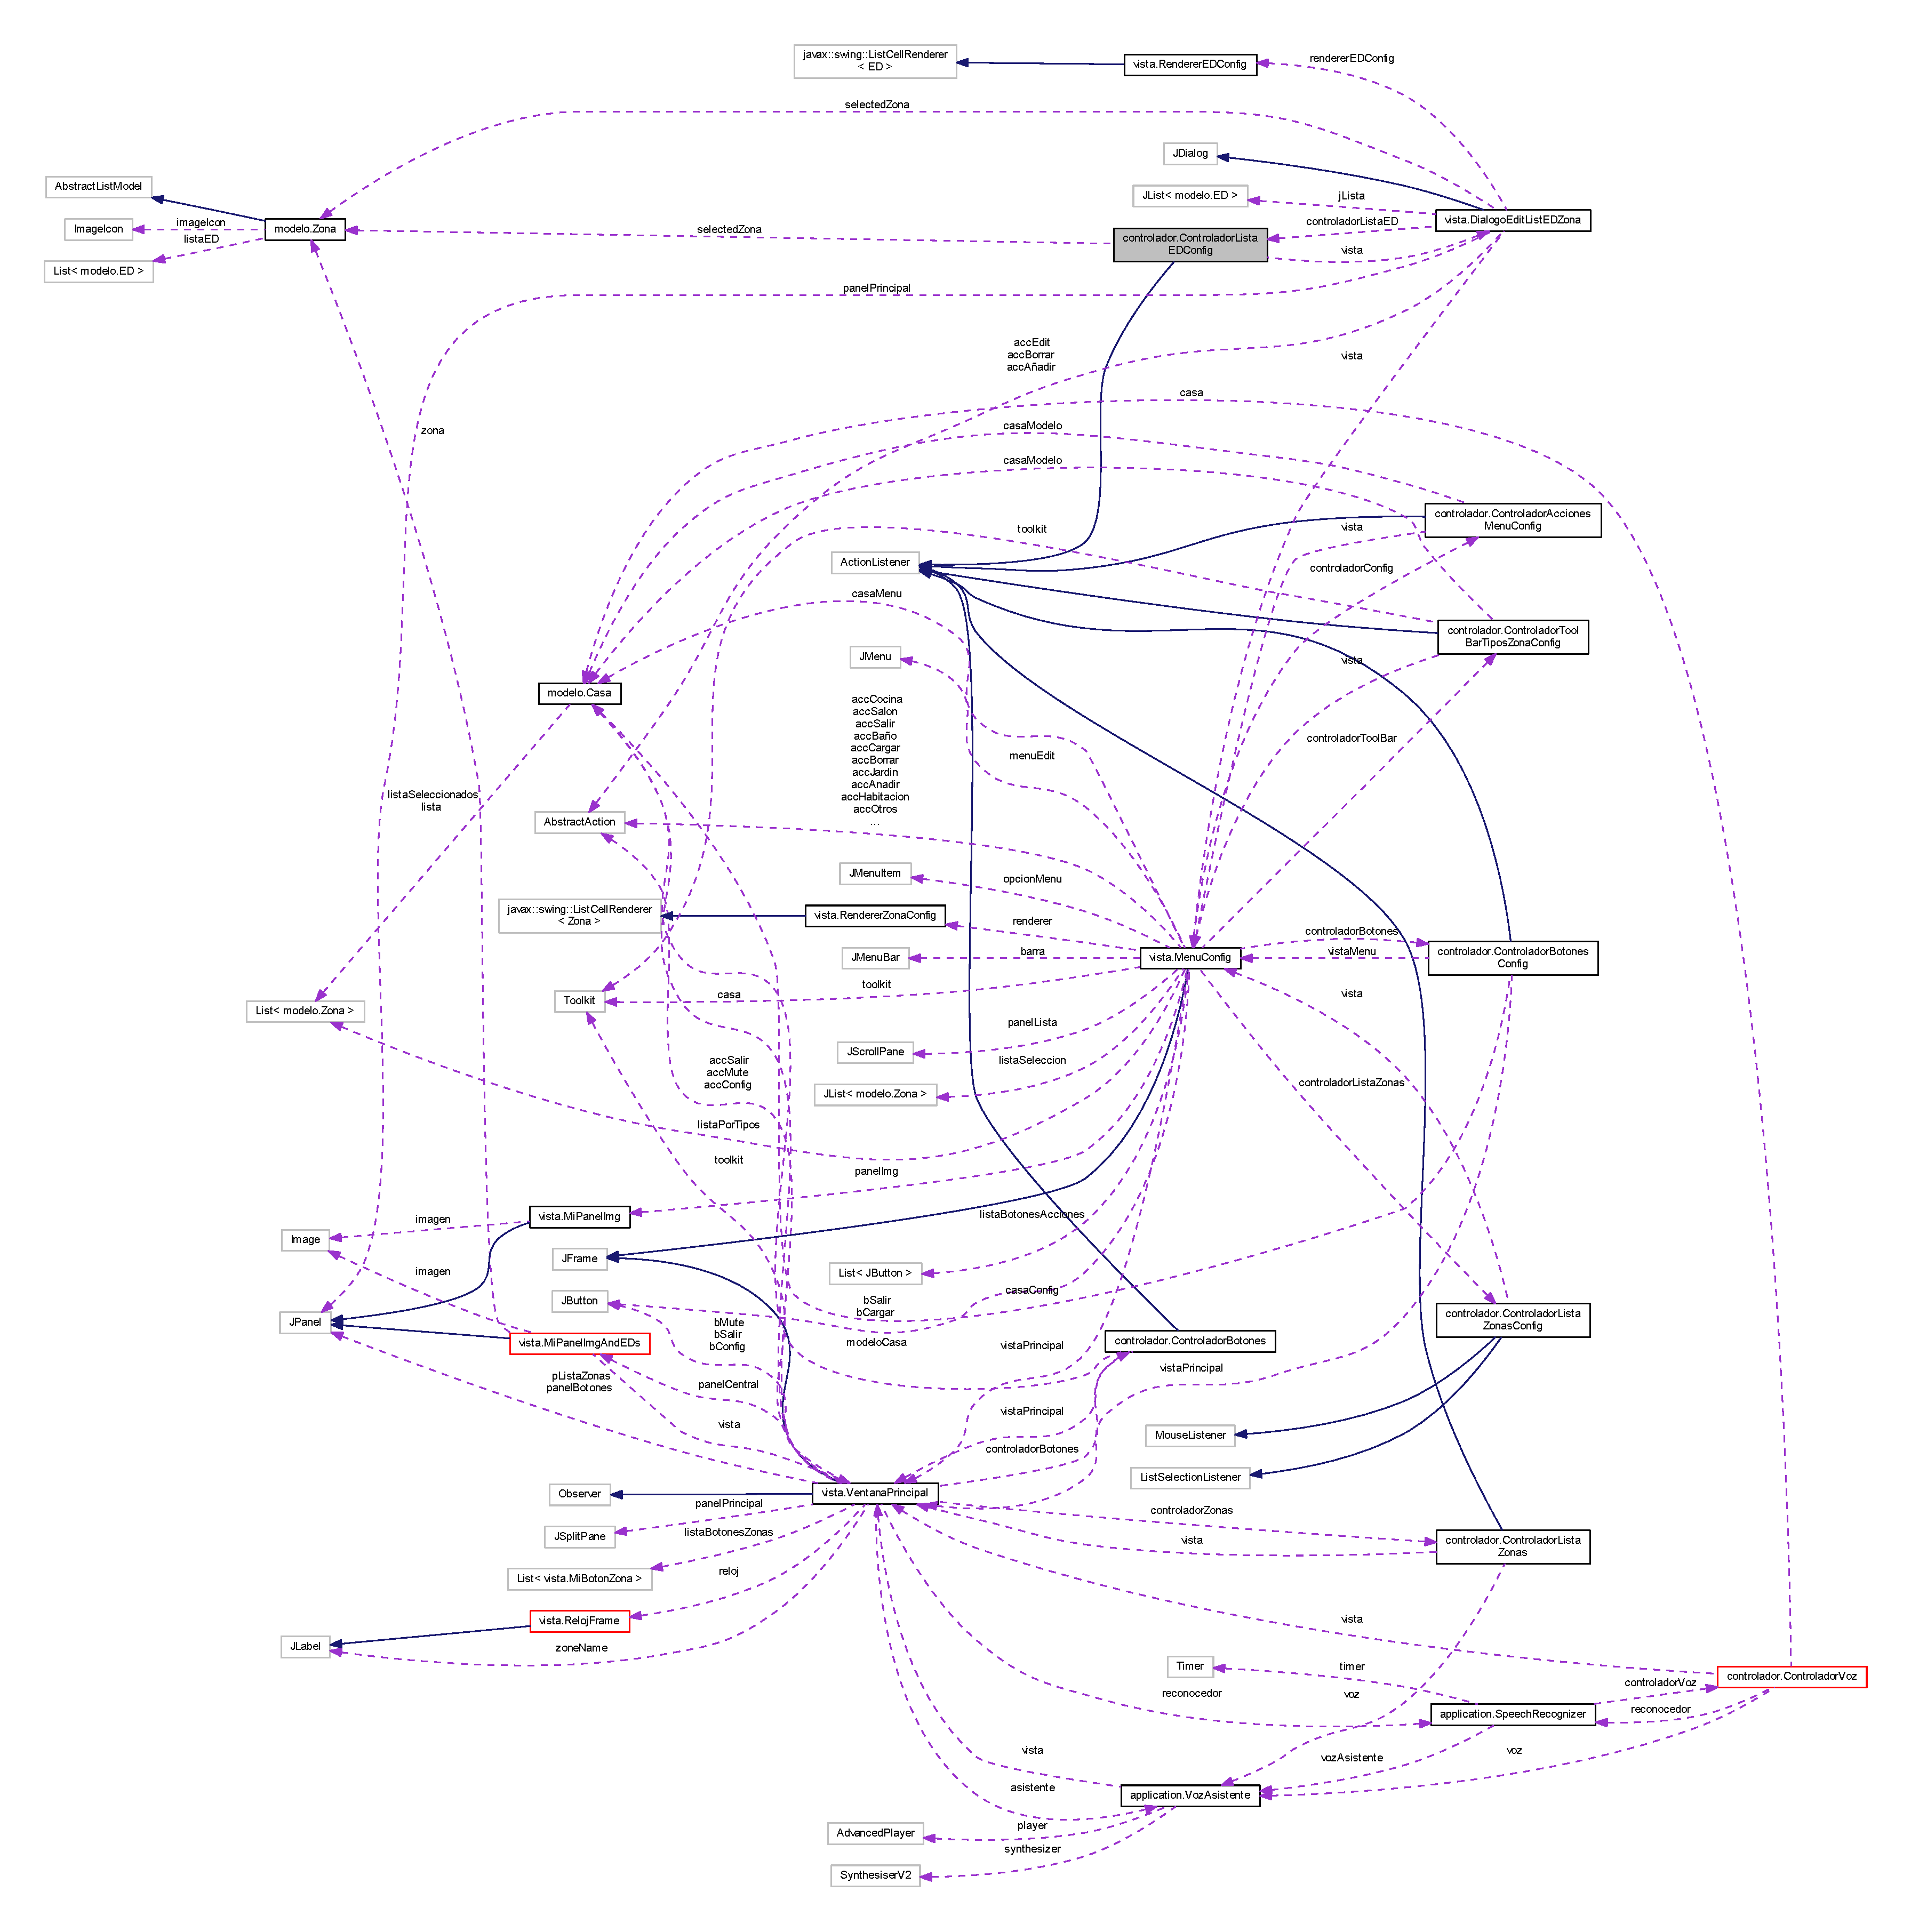
\includegraphics[width=350pt]{classcontrolador_1_1_controlador_lista_e_d_config__coll__graph}
\end{center}
\end{figure}
\subsection*{Public Member Functions}
\begin{DoxyCompactItemize}
\item 
\mbox{\Hypertarget{classcontrolador_1_1_controlador_lista_e_d_config_a041bd885847cb277021a95a25a08bc11}\label{classcontrolador_1_1_controlador_lista_e_d_config_a041bd885847cb277021a95a25a08bc11}} 
{\bfseries Controlador\+Lista\+E\+D\+Config} (\mbox{\hyperlink{classvista_1_1_dialogo_edit_list_e_d_zona}{Dialogo\+Edit\+List\+E\+D\+Zona}} vista, \mbox{\hyperlink{classmodelo_1_1_zona}{Zona}} selected\+Zona)
\item 
\mbox{\Hypertarget{classcontrolador_1_1_controlador_lista_e_d_config_aa409cf951eee8e6ffee0b092c2164684}\label{classcontrolador_1_1_controlador_lista_e_d_config_aa409cf951eee8e6ffee0b092c2164684}} 
void {\bfseries action\+Performed} (Action\+Event e)
\end{DoxyCompactItemize}


The documentation for this class was generated from the following file\+:\begin{DoxyCompactItemize}
\item 
C\+:/\+Users/\+Ander/\+Documents/\+Java/\+Dream\+Housev2/src/controlador/Controlador\+Lista\+E\+D\+Config.\+java\end{DoxyCompactItemize}

\hypertarget{classcontrolador_1_1_controlador_lista_zonas}{}\section{controlador.\+Controlador\+Lista\+Zonas Class Reference}
\label{classcontrolador_1_1_controlador_lista_zonas}\index{controlador.\+Controlador\+Lista\+Zonas@{controlador.\+Controlador\+Lista\+Zonas}}


Inheritance diagram for controlador.\+Controlador\+Lista\+Zonas\+:
\nopagebreak
\begin{figure}[H]
\begin{center}
\leavevmode
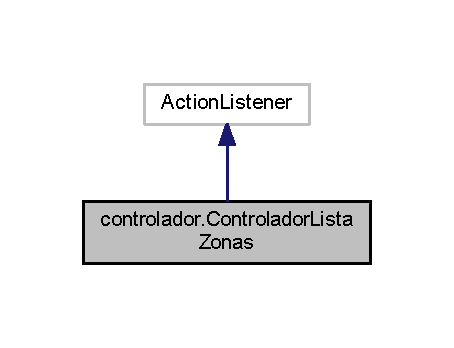
\includegraphics[width=218pt]{classcontrolador_1_1_controlador_lista_zonas__inherit__graph}
\end{center}
\end{figure}


Collaboration diagram for controlador.\+Controlador\+Lista\+Zonas\+:
\nopagebreak
\begin{figure}[H]
\begin{center}
\leavevmode
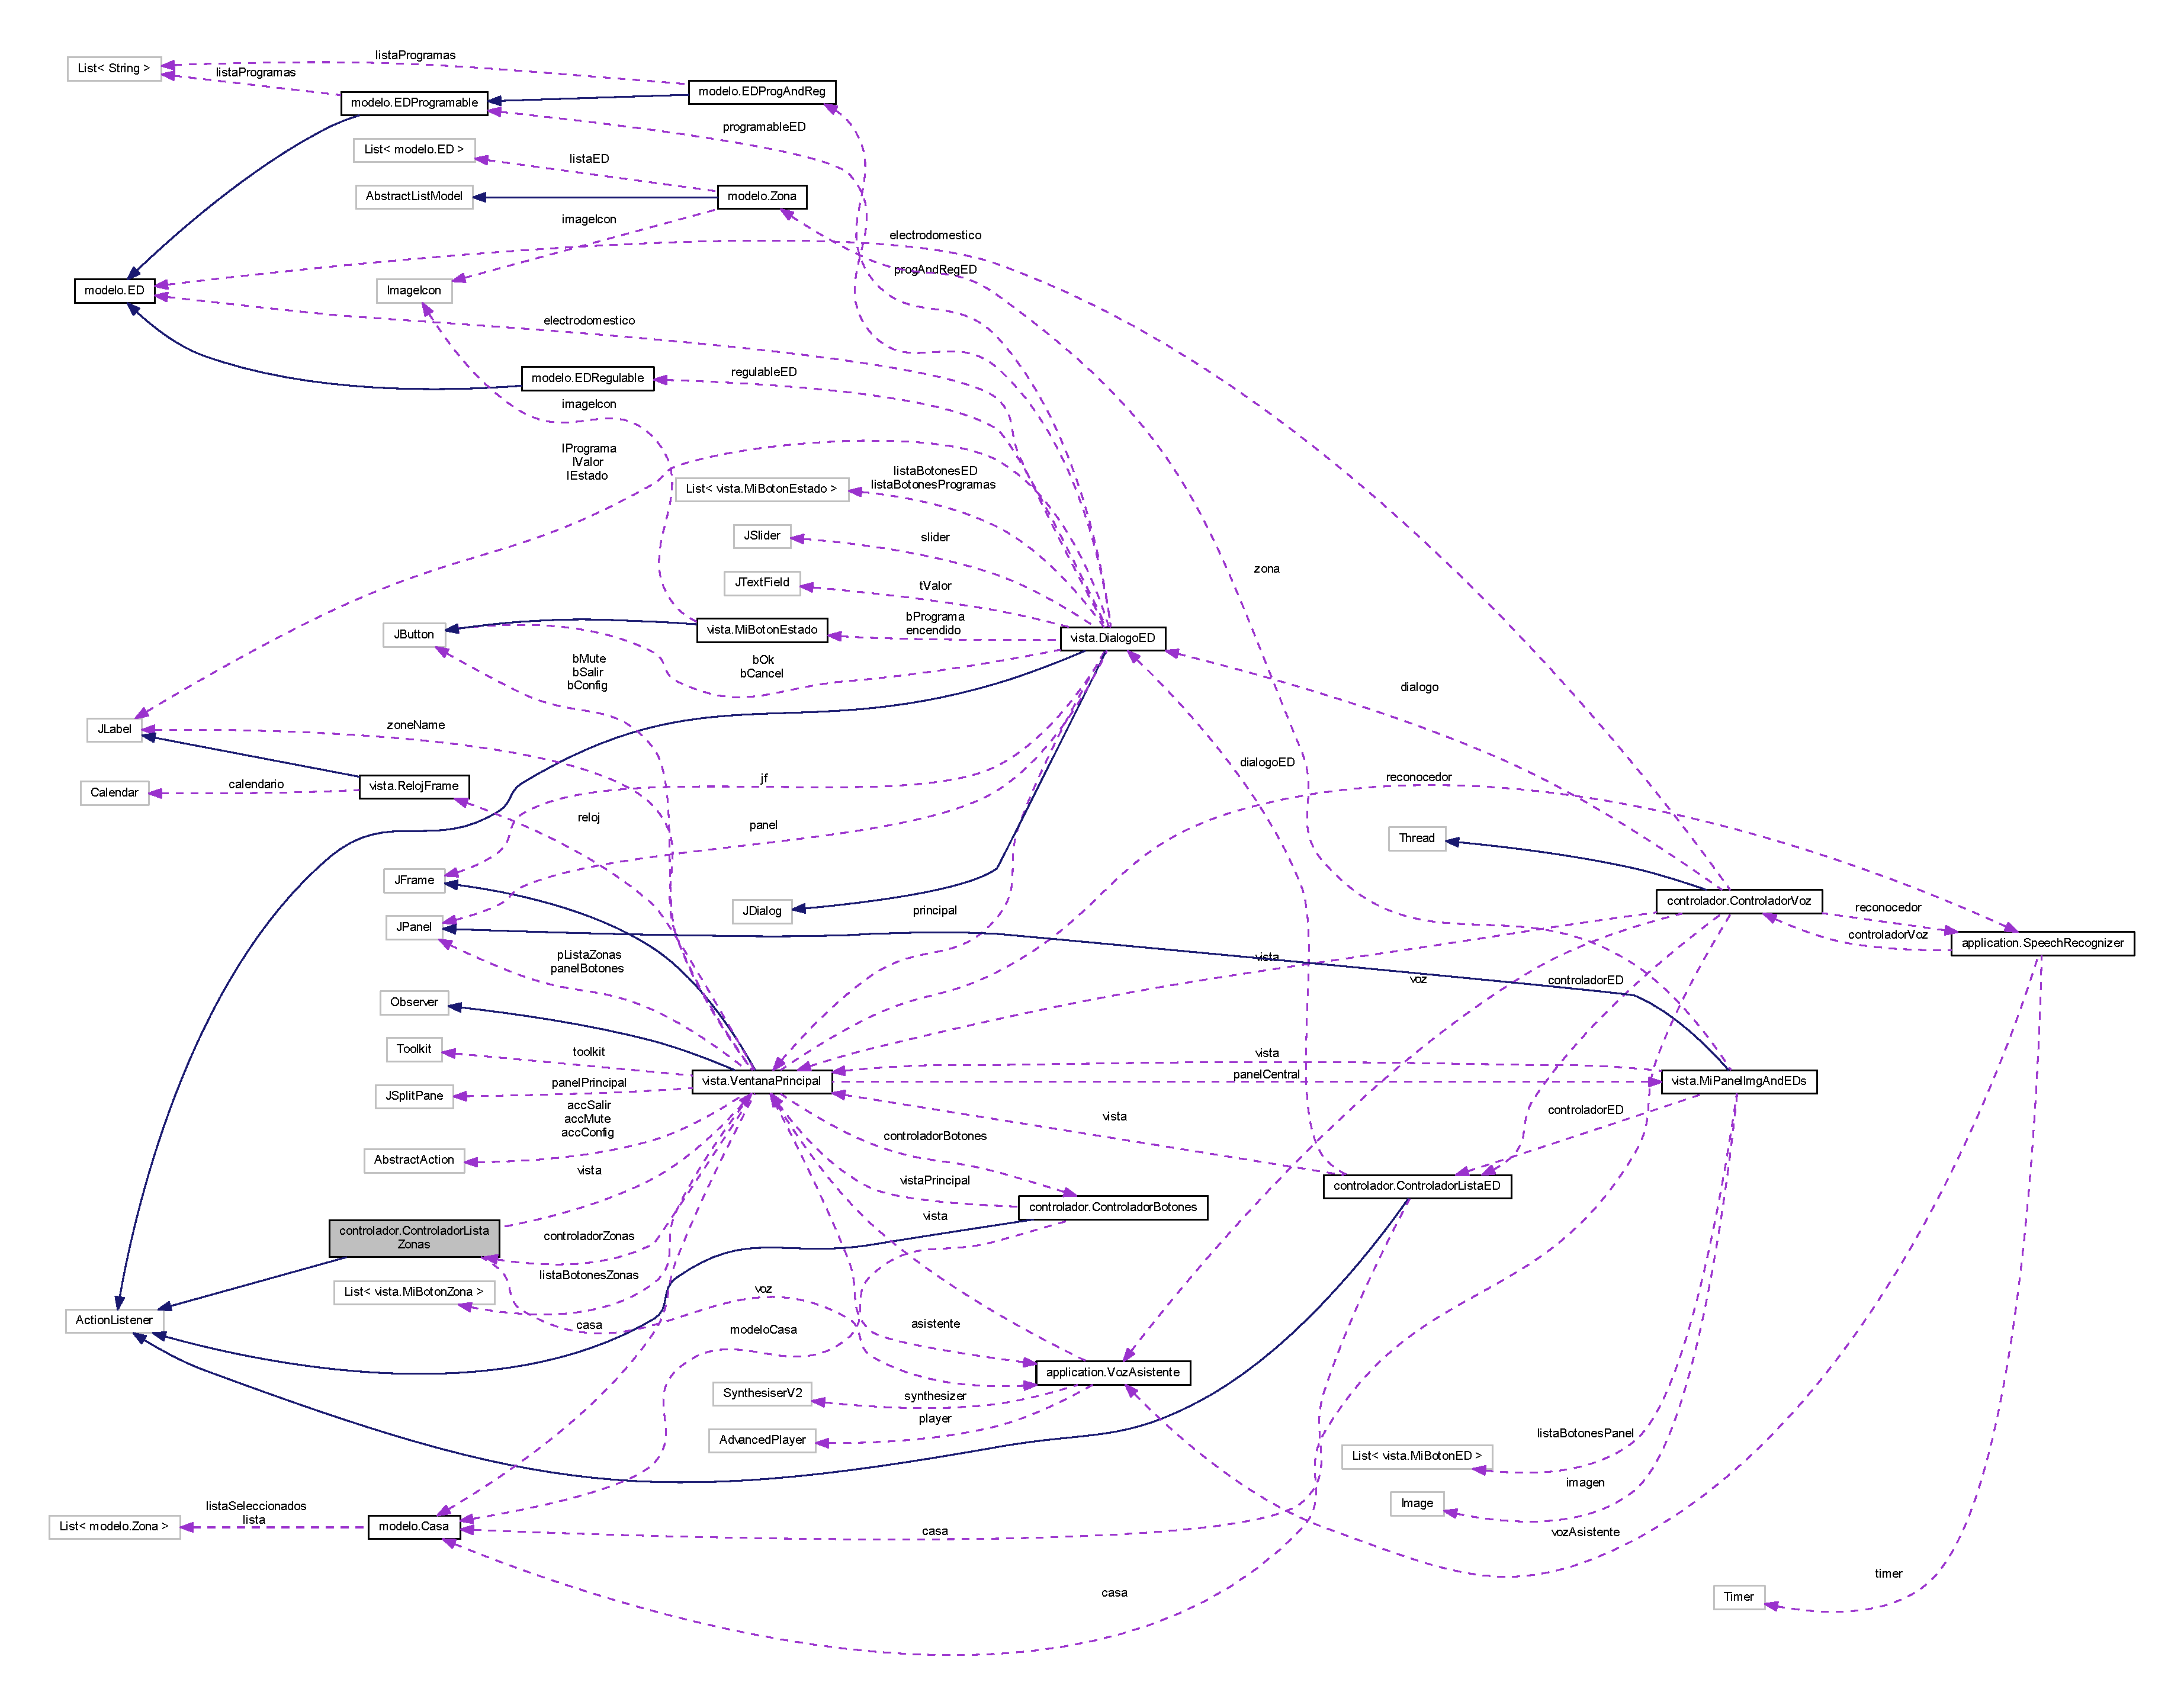
\includegraphics[width=350pt]{classcontrolador_1_1_controlador_lista_zonas__coll__graph}
\end{center}
\end{figure}
\subsection*{Public Member Functions}
\begin{DoxyCompactItemize}
\item 
\mbox{\Hypertarget{classcontrolador_1_1_controlador_lista_zonas_ace36c2e2e48aae483239b91ccc33d580}\label{classcontrolador_1_1_controlador_lista_zonas_ace36c2e2e48aae483239b91ccc33d580}} 
{\bfseries Controlador\+Lista\+Zonas} (\mbox{\hyperlink{classvista_1_1_ventana_principal}{Ventana\+Principal}} vista)
\item 
\mbox{\Hypertarget{classcontrolador_1_1_controlador_lista_zonas_a3daf75a60ff207317353b31ac649d147}\label{classcontrolador_1_1_controlador_lista_zonas_a3daf75a60ff207317353b31ac649d147}} 
void {\bfseries action\+Performed} (Action\+Event e)
\end{DoxyCompactItemize}


The documentation for this class was generated from the following file\+:\begin{DoxyCompactItemize}
\item 
C\+:/\+Users/\+Ander/\+Documents/\+Java/\+Dream\+Housev2/src/controlador/Controlador\+Lista\+Zonas.\+java\end{DoxyCompactItemize}

\hypertarget{classcontrolador_1_1_controlador_lista_zonas_config}{}\section{controlador.\+Controlador\+Lista\+Zonas\+Config Class Reference}
\label{classcontrolador_1_1_controlador_lista_zonas_config}\index{controlador.\+Controlador\+Lista\+Zonas\+Config@{controlador.\+Controlador\+Lista\+Zonas\+Config}}


Inheritance diagram for controlador.\+Controlador\+Lista\+Zonas\+Config\+:
\nopagebreak
\begin{figure}[H]
\begin{center}
\leavevmode
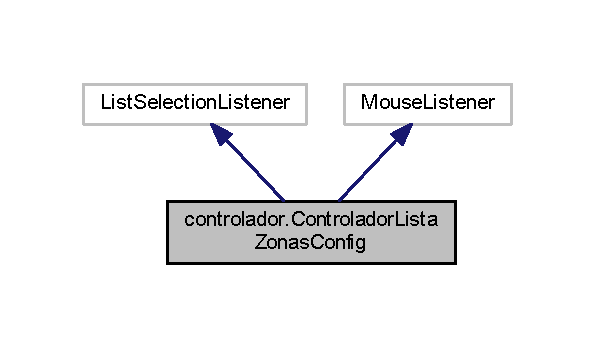
\includegraphics[width=286pt]{classcontrolador_1_1_controlador_lista_zonas_config__inherit__graph}
\end{center}
\end{figure}


Collaboration diagram for controlador.\+Controlador\+Lista\+Zonas\+Config\+:
\nopagebreak
\begin{figure}[H]
\begin{center}
\leavevmode
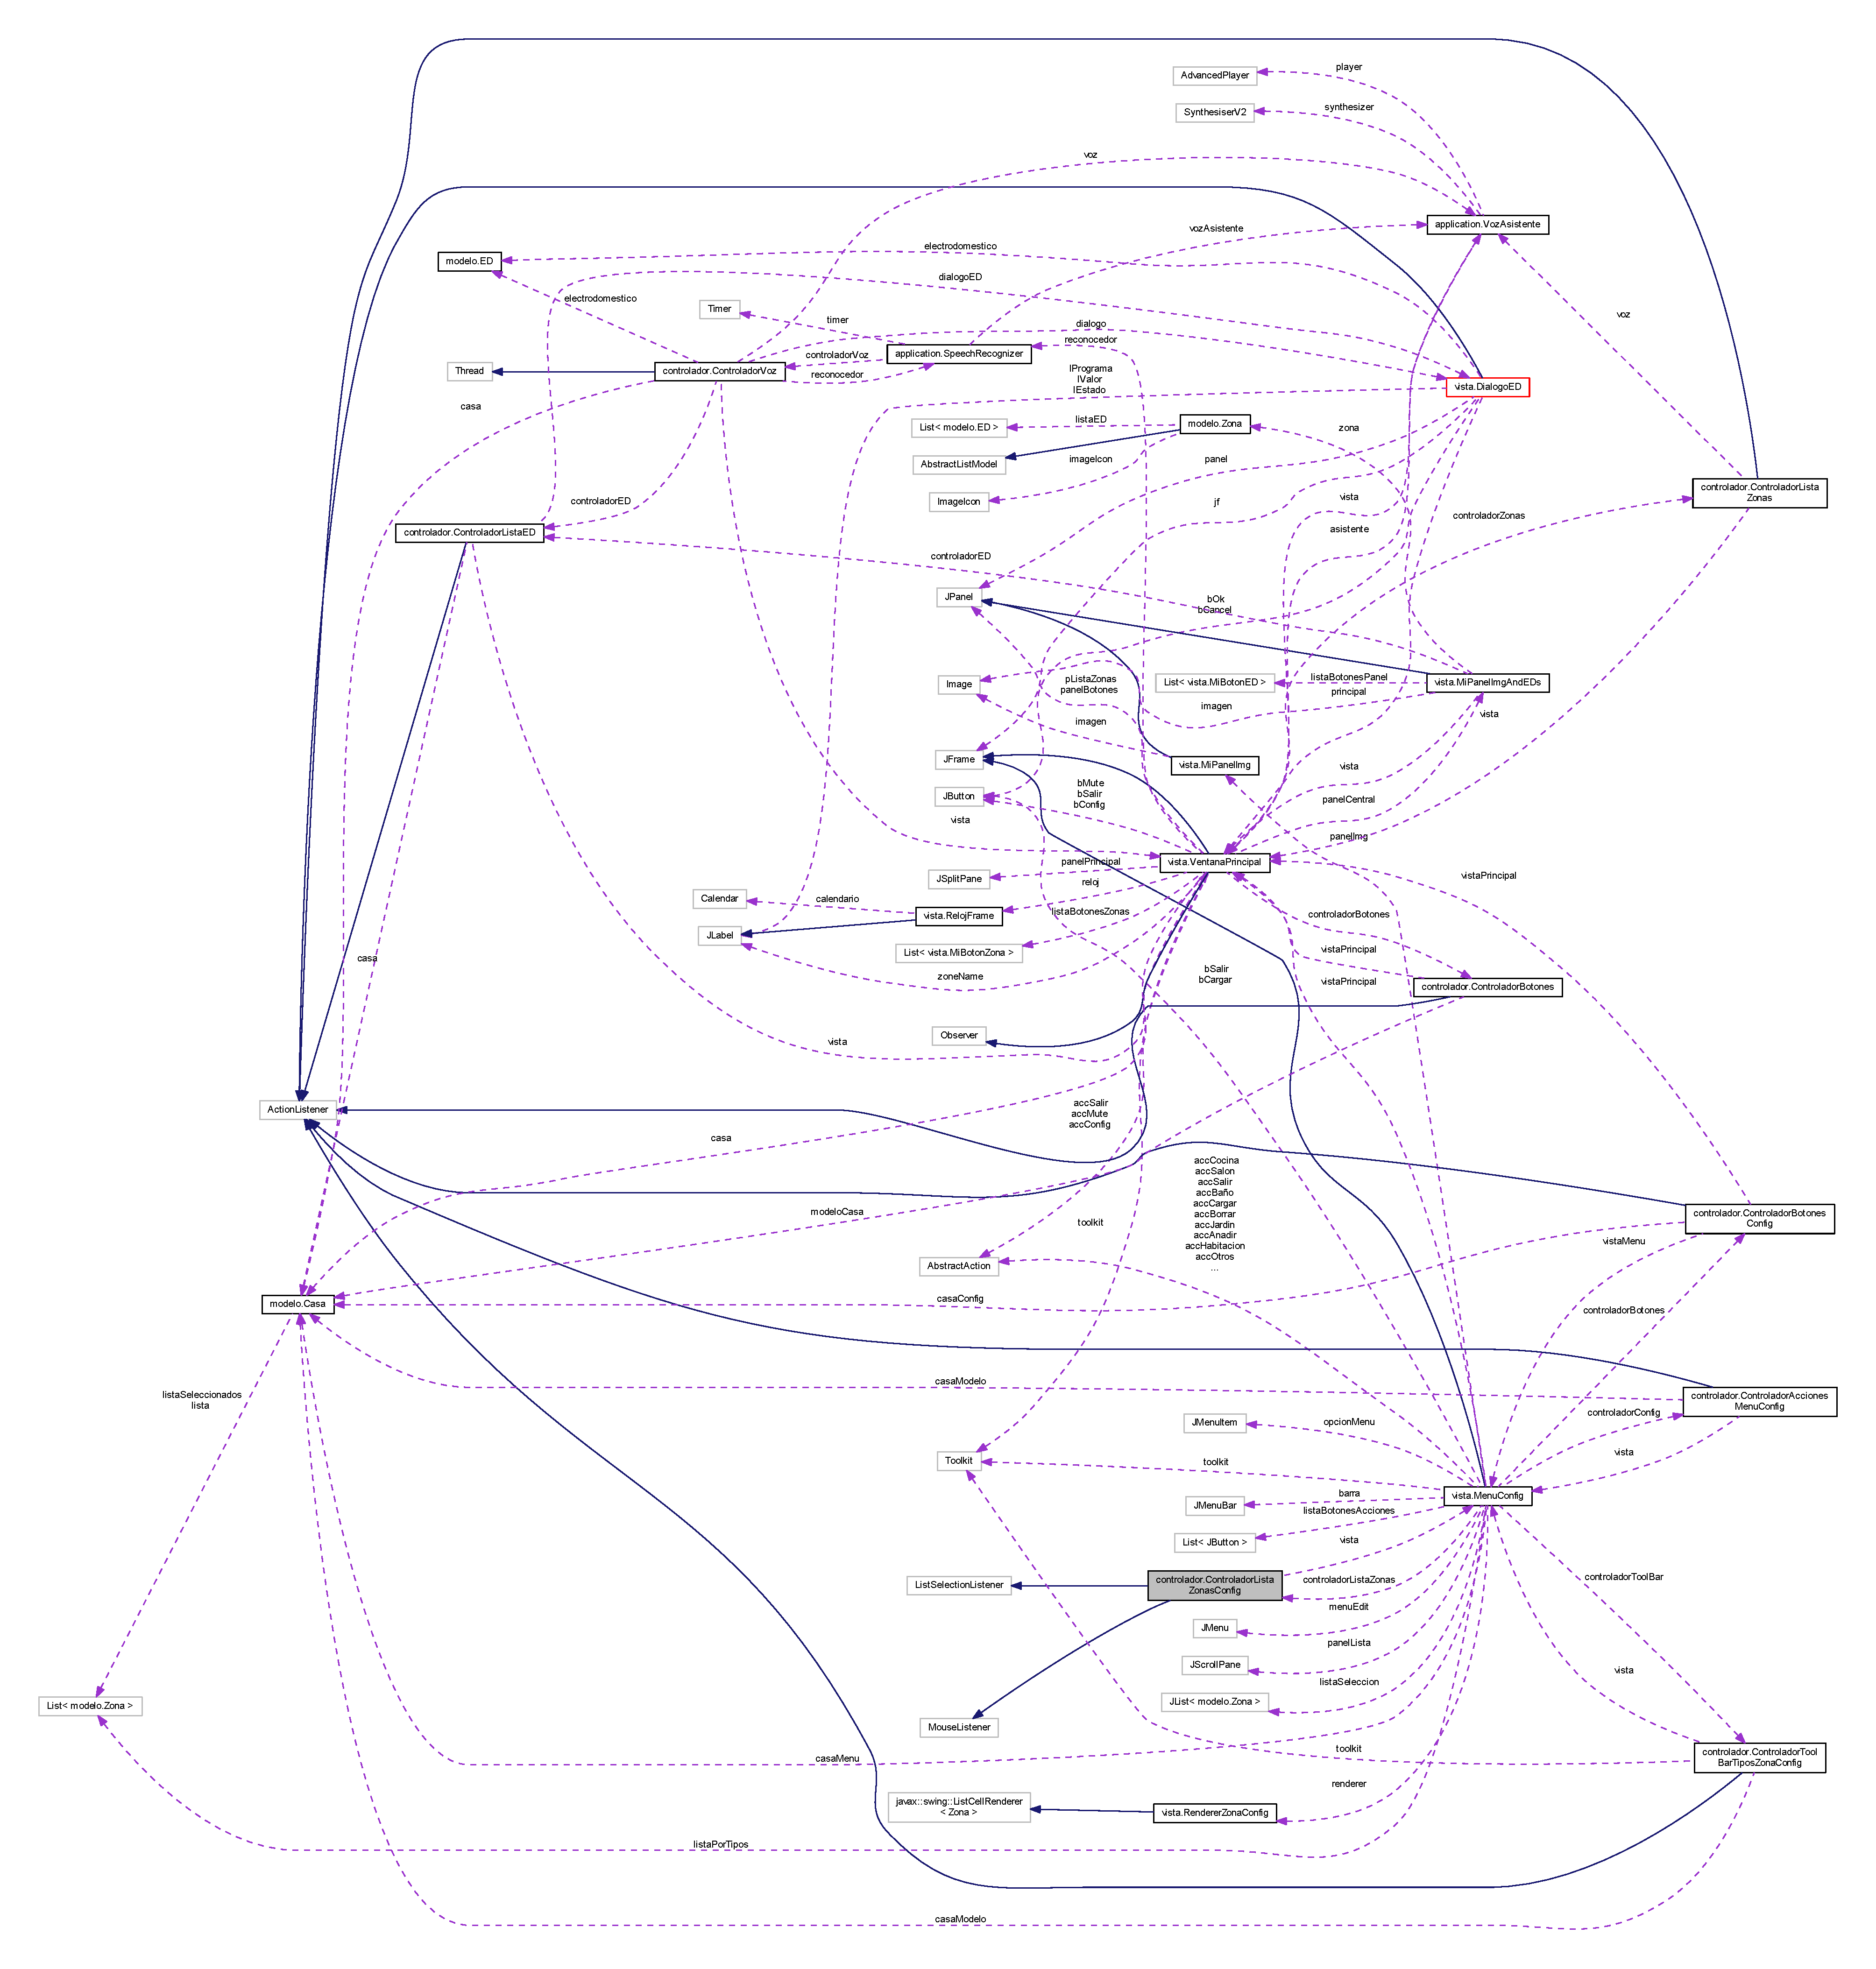
\includegraphics[width=350pt]{classcontrolador_1_1_controlador_lista_zonas_config__coll__graph}
\end{center}
\end{figure}
\subsection*{Public Member Functions}
\begin{DoxyCompactItemize}
\item 
\mbox{\Hypertarget{classcontrolador_1_1_controlador_lista_zonas_config_acfb911e40132c6189327faa9245c65d1}\label{classcontrolador_1_1_controlador_lista_zonas_config_acfb911e40132c6189327faa9245c65d1}} 
{\bfseries Controlador\+Lista\+Zonas\+Config} (\mbox{\hyperlink{classvista_1_1_menu_config}{Menu\+Config}} vista)
\item 
\mbox{\Hypertarget{classcontrolador_1_1_controlador_lista_zonas_config_a287715d558e3480db8c1e8d44dffadc1}\label{classcontrolador_1_1_controlador_lista_zonas_config_a287715d558e3480db8c1e8d44dffadc1}} 
void {\bfseries value\+Changed} (List\+Selection\+Event e)
\item 
\mbox{\Hypertarget{classcontrolador_1_1_controlador_lista_zonas_config_af9773dcae8ecdd67d09d19d35fdedb4d}\label{classcontrolador_1_1_controlador_lista_zonas_config_af9773dcae8ecdd67d09d19d35fdedb4d}} 
void {\bfseries mouse\+Clicked} (Mouse\+Event e)
\item 
\mbox{\Hypertarget{classcontrolador_1_1_controlador_lista_zonas_config_a898fa52ad57e7e6b3d5350815718430d}\label{classcontrolador_1_1_controlador_lista_zonas_config_a898fa52ad57e7e6b3d5350815718430d}} 
void {\bfseries mouse\+Entered} (Mouse\+Event arg0)
\item 
\mbox{\Hypertarget{classcontrolador_1_1_controlador_lista_zonas_config_a423eb2c5ec368f656f37f7b585ac8e23}\label{classcontrolador_1_1_controlador_lista_zonas_config_a423eb2c5ec368f656f37f7b585ac8e23}} 
void {\bfseries mouse\+Exited} (Mouse\+Event arg0)
\item 
\mbox{\Hypertarget{classcontrolador_1_1_controlador_lista_zonas_config_ad8103d85ca6edb1ac19d3914d4655462}\label{classcontrolador_1_1_controlador_lista_zonas_config_ad8103d85ca6edb1ac19d3914d4655462}} 
void {\bfseries mouse\+Pressed} (Mouse\+Event arg0)
\item 
\mbox{\Hypertarget{classcontrolador_1_1_controlador_lista_zonas_config_a34ccbeec87ff186869925224f4877821}\label{classcontrolador_1_1_controlador_lista_zonas_config_a34ccbeec87ff186869925224f4877821}} 
void {\bfseries mouse\+Released} (Mouse\+Event arg0)
\end{DoxyCompactItemize}


The documentation for this class was generated from the following file\+:\begin{DoxyCompactItemize}
\item 
C\+:/\+Users/\+Ander/\+Documents/\+Java/\+Dream\+Housev2/src/controlador/Controlador\+Lista\+Zonas\+Config.\+java\end{DoxyCompactItemize}

\hypertarget{classcontrolador_1_1_controlador_tool_bar_tipos_zona_config}{}\section{controlador.\+Controlador\+Tool\+Bar\+Tipos\+Zona\+Config Class Reference}
\label{classcontrolador_1_1_controlador_tool_bar_tipos_zona_config}\index{controlador.\+Controlador\+Tool\+Bar\+Tipos\+Zona\+Config@{controlador.\+Controlador\+Tool\+Bar\+Tipos\+Zona\+Config}}


Inheritance diagram for controlador.\+Controlador\+Tool\+Bar\+Tipos\+Zona\+Config\+:
\nopagebreak
\begin{figure}[H]
\begin{center}
\leavevmode
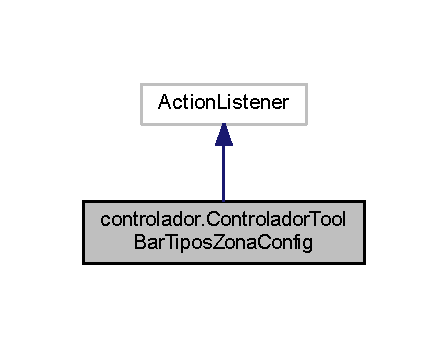
\includegraphics[width=215pt]{classcontrolador_1_1_controlador_tool_bar_tipos_zona_config__inherit__graph}
\end{center}
\end{figure}


Collaboration diagram for controlador.\+Controlador\+Tool\+Bar\+Tipos\+Zona\+Config\+:
\nopagebreak
\begin{figure}[H]
\begin{center}
\leavevmode
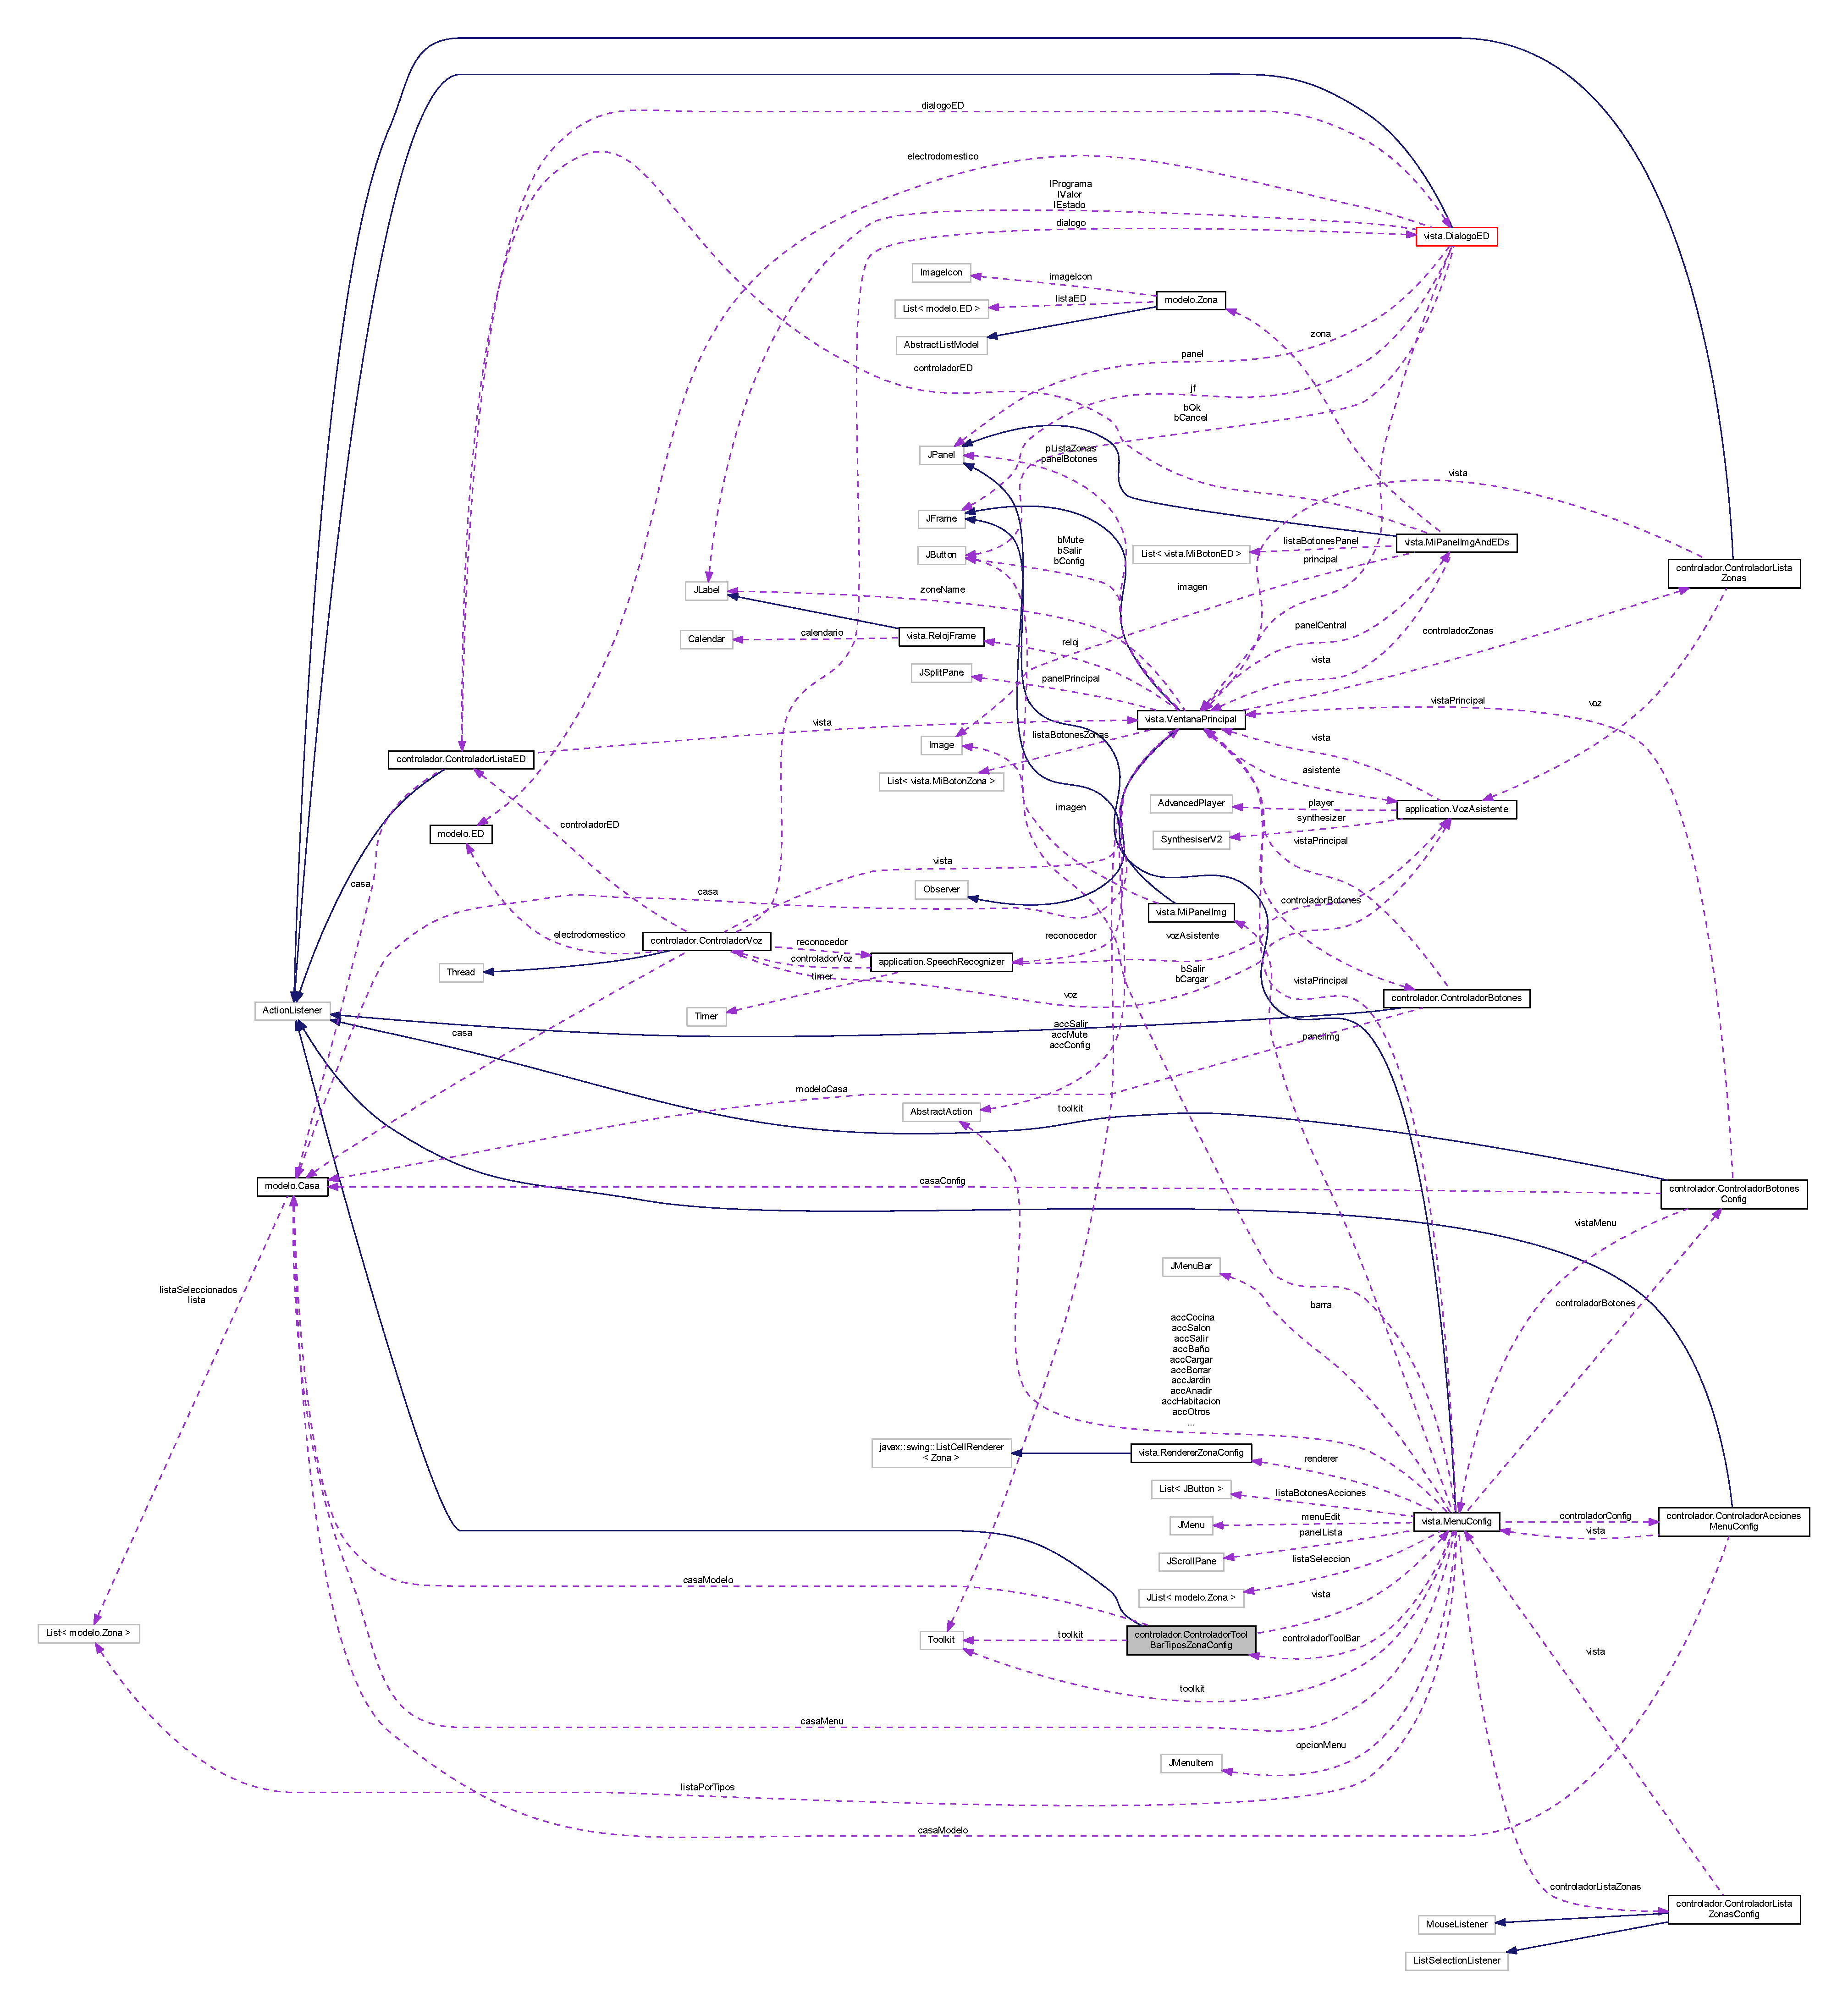
\includegraphics[width=350pt]{classcontrolador_1_1_controlador_tool_bar_tipos_zona_config__coll__graph}
\end{center}
\end{figure}
\subsection*{Public Member Functions}
\begin{DoxyCompactItemize}
\item 
\mbox{\Hypertarget{classcontrolador_1_1_controlador_tool_bar_tipos_zona_config_abe5f20494136e5255907b56cc2b84fe1}\label{classcontrolador_1_1_controlador_tool_bar_tipos_zona_config_abe5f20494136e5255907b56cc2b84fe1}} 
{\bfseries Controlador\+Tool\+Bar\+Tipos\+Zona\+Config} (\mbox{\hyperlink{classvista_1_1_menu_config}{Menu\+Config}} vista, \mbox{\hyperlink{classmodelo_1_1_casa}{Casa}} modelo)
\item 
\mbox{\Hypertarget{classcontrolador_1_1_controlador_tool_bar_tipos_zona_config_a4a1a33dc6048a80803fea31e42b77068}\label{classcontrolador_1_1_controlador_tool_bar_tipos_zona_config_a4a1a33dc6048a80803fea31e42b77068}} 
void {\bfseries action\+Performed} (Action\+Event e)
\end{DoxyCompactItemize}


The documentation for this class was generated from the following file\+:\begin{DoxyCompactItemize}
\item 
C\+:/\+Users/\+Ander/\+Documents/\+Java/\+Dream\+Housev2/src/controlador/Controlador\+Tool\+Bar\+Tipos\+Zona\+Config.\+java\end{DoxyCompactItemize}

\hypertarget{classcontrolador_1_1_controlador_voz}{}\section{controlador.\+Controlador\+Voz Class Reference}
\label{classcontrolador_1_1_controlador_voz}\index{controlador.\+Controlador\+Voz@{controlador.\+Controlador\+Voz}}


Inheritance diagram for controlador.\+Controlador\+Voz\+:
\nopagebreak
\begin{figure}[H]
\begin{center}
\leavevmode
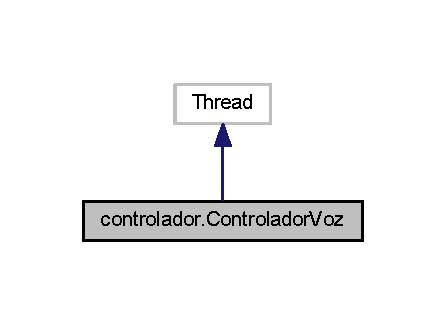
\includegraphics[width=214pt]{classcontrolador_1_1_controlador_voz__inherit__graph}
\end{center}
\end{figure}


Collaboration diagram for controlador.\+Controlador\+Voz\+:
\nopagebreak
\begin{figure}[H]
\begin{center}
\leavevmode
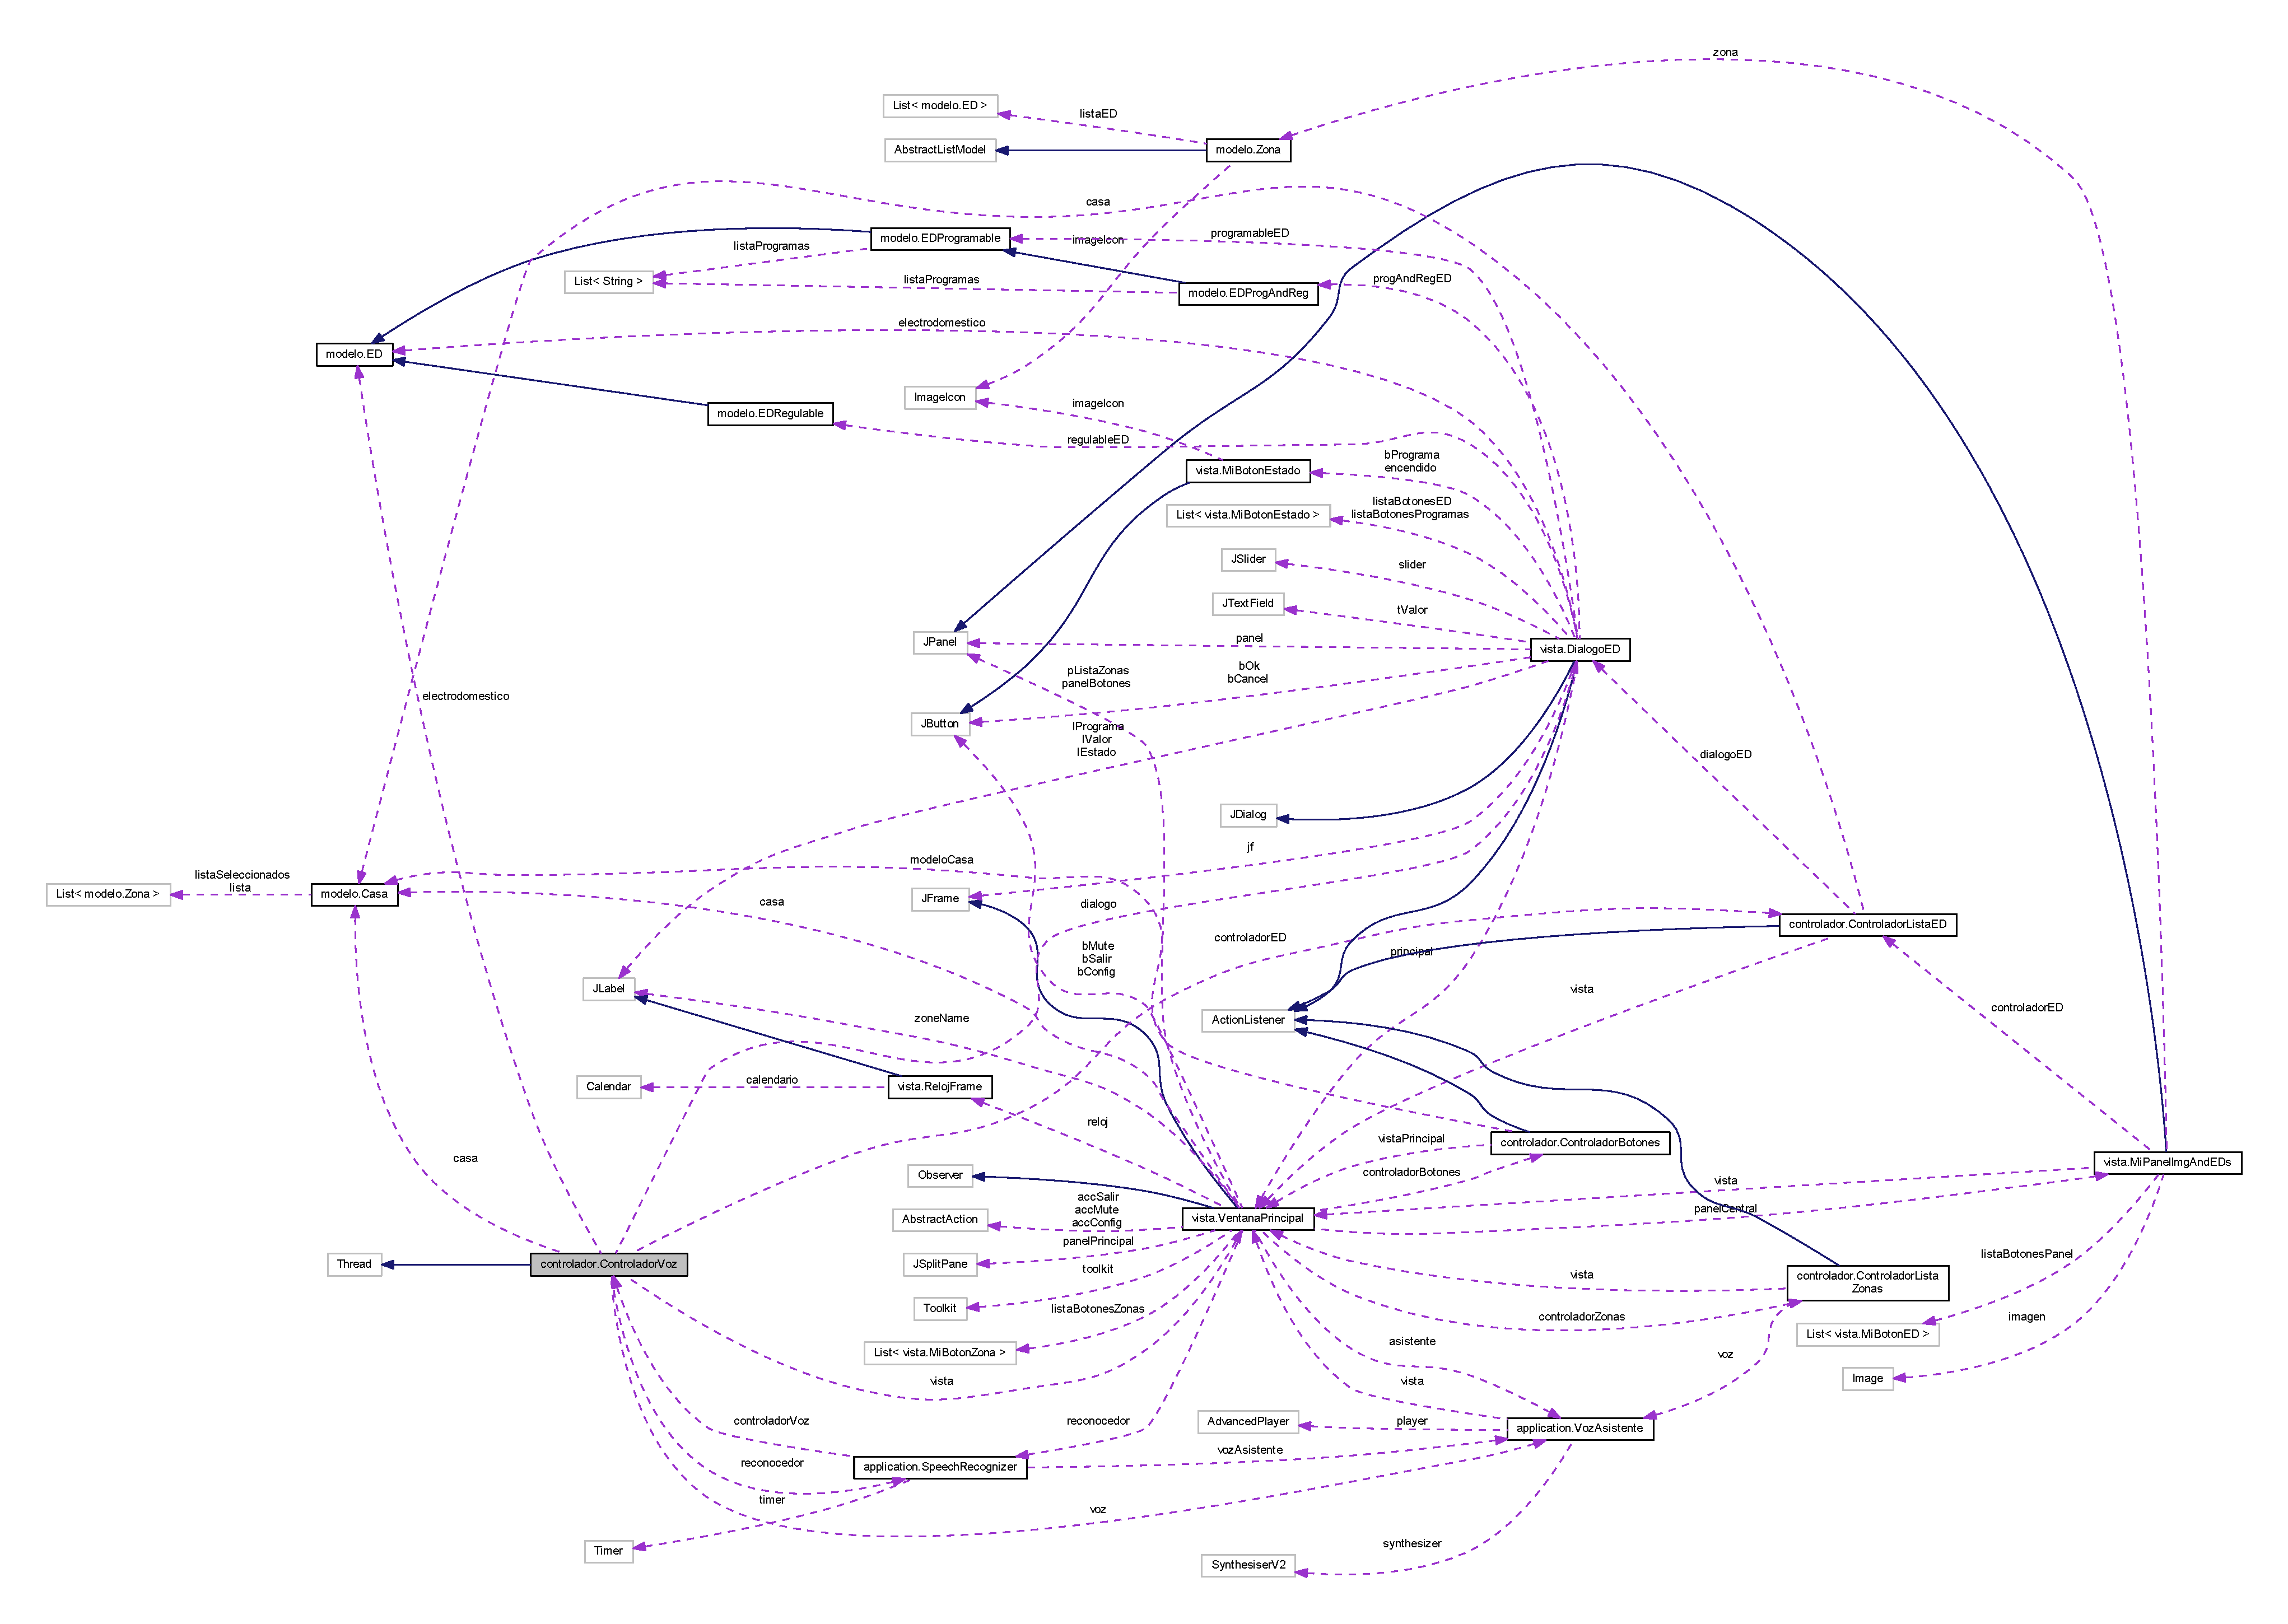
\includegraphics[width=350pt]{classcontrolador_1_1_controlador_voz__coll__graph}
\end{center}
\end{figure}
\subsection*{Public Member Functions}
\begin{DoxyCompactItemize}
\item 
\mbox{\Hypertarget{classcontrolador_1_1_controlador_voz_a6cda936ee3d81085740a81c018803bf7}\label{classcontrolador_1_1_controlador_voz_a6cda936ee3d81085740a81c018803bf7}} 
{\bfseries Controlador\+Voz} (\mbox{\hyperlink{classvista_1_1_ventana_principal}{Ventana\+Principal}} vista, \mbox{\hyperlink{classmodelo_1_1_casa}{Casa}} casa)
\item 
\mbox{\Hypertarget{classcontrolador_1_1_controlador_voz_a77d8d66f1bbe3174d4df8a5c171cc4c5}\label{classcontrolador_1_1_controlador_voz_a77d8d66f1bbe3174d4df8a5c171cc4c5}} 
void {\bfseries filtrador\+Zonas} (String palabra)
\item 
\mbox{\Hypertarget{classcontrolador_1_1_controlador_voz_a069bc1084f39b2c10a069731b353f6da}\label{classcontrolador_1_1_controlador_voz_a069bc1084f39b2c10a069731b353f6da}} 
String {\bfseries digit\+To\+Word} (String palabra)
\item 
\mbox{\Hypertarget{classcontrolador_1_1_controlador_voz_a7a526053d4d5fce89ad3f9bd68f39ee1}\label{classcontrolador_1_1_controlador_voz_a7a526053d4d5fce89ad3f9bd68f39ee1}} 
String {\bfseries texto\+En\+Unidad} (String palabra)
\end{DoxyCompactItemize}


The documentation for this class was generated from the following file\+:\begin{DoxyCompactItemize}
\item 
C\+:/\+Users/\+Ander/\+Documents/\+Java/\+Dream\+Housev2/src/controlador/Controlador\+Voz.\+java\end{DoxyCompactItemize}

\hypertarget{classvista_1_1_dialogo_a_xC3_xB1adir_editar_e_d}{}\section{vista.\+Dialogo\+Añadir\+Editar\+ED Class Reference}
\label{classvista_1_1_dialogo_a_xC3_xB1adir_editar_e_d}\index{vista.\+Dialogo\+Añadir\+Editar\+ED@{vista.\+Dialogo\+Añadir\+Editar\+ED}}


Inheritance diagram for vista.\+Dialogo\+Añadir\+Editar\+ED\+:
\nopagebreak
\begin{figure}[H]
\begin{center}
\leavevmode
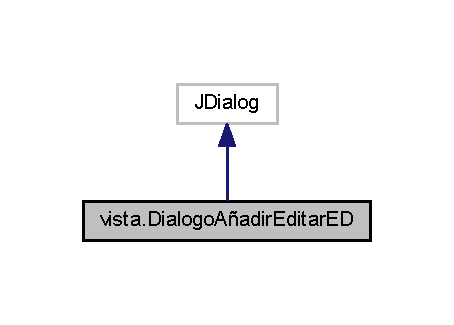
\includegraphics[width=218pt]{classvista_1_1_dialogo_a_xC3_xB1adir_editar_e_d__inherit__graph}
\end{center}
\end{figure}


Collaboration diagram for vista.\+Dialogo\+Añadir\+Editar\+ED\+:
\nopagebreak
\begin{figure}[H]
\begin{center}
\leavevmode
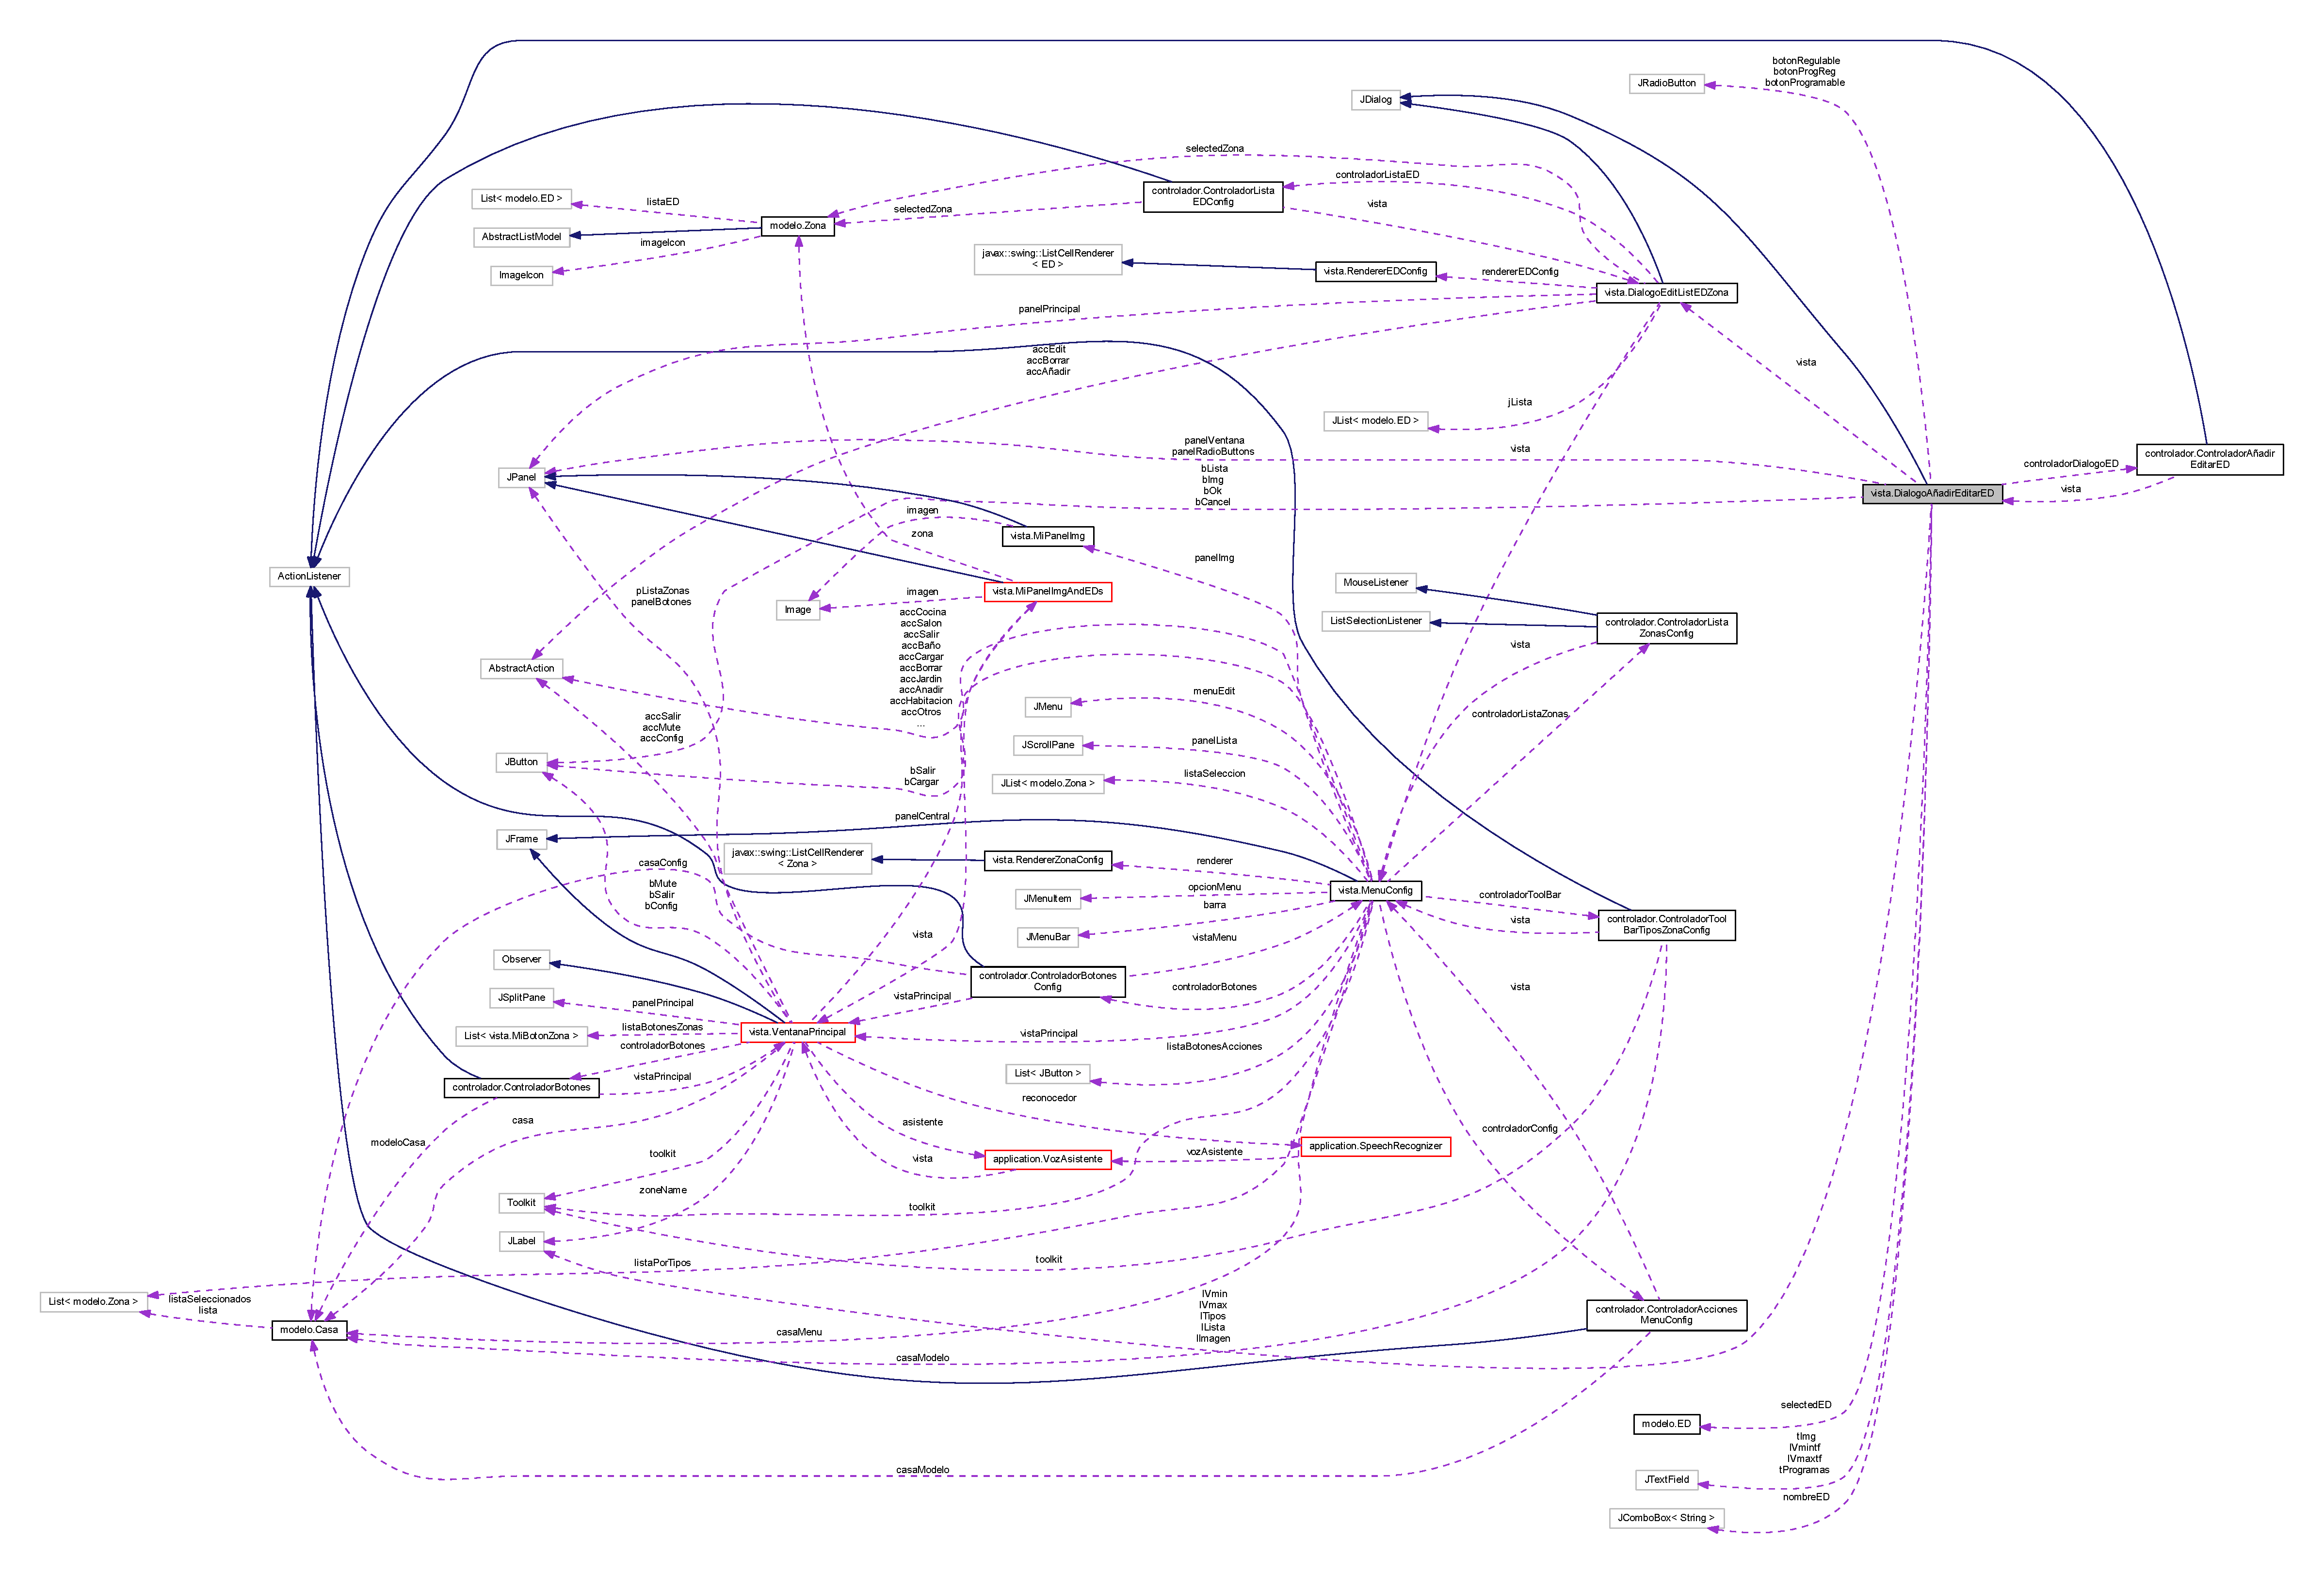
\includegraphics[width=350pt]{classvista_1_1_dialogo_a_xC3_xB1adir_editar_e_d__coll__graph}
\end{center}
\end{figure}
\subsection*{Public Member Functions}
\begin{DoxyCompactItemize}
\item 
\mbox{\Hypertarget{classvista_1_1_dialogo_a_xC3_xB1adir_editar_e_d_a6eee77dd9a1cefe1069f58a427ea720e}\label{classvista_1_1_dialogo_a_xC3_xB1adir_editar_e_d_a6eee77dd9a1cefe1069f58a427ea720e}} 
{\bfseries Dialogo\+Añadir\+Editar\+ED} (\mbox{\hyperlink{classvista_1_1_dialogo_edit_list_e_d_zona}{Dialogo\+Edit\+List\+E\+D\+Zona}} ventana, String titulo, boolean modo, boolean esta\+Añadiendo)
\item 
\mbox{\Hypertarget{classvista_1_1_dialogo_a_xC3_xB1adir_editar_e_d_a8fc12de0e1c8f392d5bfb9c536b08681}\label{classvista_1_1_dialogo_a_xC3_xB1adir_editar_e_d_a8fc12de0e1c8f392d5bfb9c536b08681}} 
boolean {\bfseries is\+Esta\+Añadiendo} ()
\item 
\mbox{\Hypertarget{classvista_1_1_dialogo_a_xC3_xB1adir_editar_e_d_a07093fd106d820f76588c874aba95cc1}\label{classvista_1_1_dialogo_a_xC3_xB1adir_editar_e_d_a07093fd106d820f76588c874aba95cc1}} 
J\+Combo\+Box {\bfseries get\+Nombre\+ED} ()
\item 
\mbox{\Hypertarget{classvista_1_1_dialogo_a_xC3_xB1adir_editar_e_d_a117c2dfd237e5bc25fc4e49f531dcaab}\label{classvista_1_1_dialogo_a_xC3_xB1adir_editar_e_d_a117c2dfd237e5bc25fc4e49f531dcaab}} 
void {\bfseries set\+Everything} (String tipo)
\item 
\mbox{\Hypertarget{classvista_1_1_dialogo_a_xC3_xB1adir_editar_e_d_a8da67d26b1a48c253fdc8c7bd4424d74}\label{classvista_1_1_dialogo_a_xC3_xB1adir_editar_e_d_a8da67d26b1a48c253fdc8c7bd4424d74}} 
Button\+Group {\bfseries get\+Group} ()
\item 
\mbox{\Hypertarget{classvista_1_1_dialogo_a_xC3_xB1adir_editar_e_d_a57e203c700fd371e0bebd55c8b347c07}\label{classvista_1_1_dialogo_a_xC3_xB1adir_editar_e_d_a57e203c700fd371e0bebd55c8b347c07}} 
J\+Radio\+Button {\bfseries get\+Selected\+Radio\+Button} ()
\item 
\mbox{\Hypertarget{classvista_1_1_dialogo_a_xC3_xB1adir_editar_e_d_aa7d9b9ec930df09cb84dd3336f121688}\label{classvista_1_1_dialogo_a_xC3_xB1adir_editar_e_d_aa7d9b9ec930df09cb84dd3336f121688}} 
String \mbox{[}$\,$\mbox{]} {\bfseries get\+Opciones\+Normal} ()
\item 
\mbox{\Hypertarget{classvista_1_1_dialogo_a_xC3_xB1adir_editar_e_d_acbbbc6b7ab5d077466db0fd993c9364d}\label{classvista_1_1_dialogo_a_xC3_xB1adir_editar_e_d_acbbbc6b7ab5d077466db0fd993c9364d}} 
String \mbox{[}$\,$\mbox{]} {\bfseries get\+Opciones\+Regulable} ()
\item 
\mbox{\Hypertarget{classvista_1_1_dialogo_a_xC3_xB1adir_editar_e_d_a454167bccc99ac3a89b5a2a4104d25ab}\label{classvista_1_1_dialogo_a_xC3_xB1adir_editar_e_d_a454167bccc99ac3a89b5a2a4104d25ab}} 
String \mbox{[}$\,$\mbox{]} {\bfseries get\+Opciones\+Programable} ()
\item 
\mbox{\Hypertarget{classvista_1_1_dialogo_a_xC3_xB1adir_editar_e_d_a2773d9feaddd2fceefd790236c5fef53}\label{classvista_1_1_dialogo_a_xC3_xB1adir_editar_e_d_a2773d9feaddd2fceefd790236c5fef53}} 
String \mbox{[}$\,$\mbox{]} {\bfseries get\+Opciones\+Prog\+Reg} ()
\item 
\mbox{\Hypertarget{classvista_1_1_dialogo_a_xC3_xB1adir_editar_e_d_ab09d8c7bdcd4ec1669ea75748fdaccc1}\label{classvista_1_1_dialogo_a_xC3_xB1adir_editar_e_d_ab09d8c7bdcd4ec1669ea75748fdaccc1}} 
J\+Text\+Field {\bfseries get\+Vmaxtf} ()
\item 
\mbox{\Hypertarget{classvista_1_1_dialogo_a_xC3_xB1adir_editar_e_d_a95a4db4b81684e42edc4cb68906d56a3}\label{classvista_1_1_dialogo_a_xC3_xB1adir_editar_e_d_a95a4db4b81684e42edc4cb68906d56a3}} 
void {\bfseries set\+Fichero\+Lista\+Programas} (String fichero\+Lista\+Programas)
\item 
\mbox{\Hypertarget{classvista_1_1_dialogo_a_xC3_xB1adir_editar_e_d_a4ee7c1d76677e9870ea40819f7354684}\label{classvista_1_1_dialogo_a_xC3_xB1adir_editar_e_d_a4ee7c1d76677e9870ea40819f7354684}} 
J\+Text\+Field {\bfseries get\+Vmintf} ()
\item 
\mbox{\Hypertarget{classvista_1_1_dialogo_a_xC3_xB1adir_editar_e_d_a17ccb4ab4bde3e3709b92e1528a068bf}\label{classvista_1_1_dialogo_a_xC3_xB1adir_editar_e_d_a17ccb4ab4bde3e3709b92e1528a068bf}} 
J\+Button {\bfseries getb\+Img} ()
\item 
\mbox{\Hypertarget{classvista_1_1_dialogo_a_xC3_xB1adir_editar_e_d_a88611d926b8c42d19ab1644570190a08}\label{classvista_1_1_dialogo_a_xC3_xB1adir_editar_e_d_a88611d926b8c42d19ab1644570190a08}} 
J\+Button {\bfseries getb\+Lista} ()
\item 
\mbox{\Hypertarget{classvista_1_1_dialogo_a_xC3_xB1adir_editar_e_d_a18b53c8b25fb4c85f3dd4293720d3ecd}\label{classvista_1_1_dialogo_a_xC3_xB1adir_editar_e_d_a18b53c8b25fb4c85f3dd4293720d3ecd}} 
void {\bfseries set\+Fichero\+Imagen} (String fichero\+Imagen)
\item 
\mbox{\Hypertarget{classvista_1_1_dialogo_a_xC3_xB1adir_editar_e_d_acd30bec076e407584365c29aa9d48bc6}\label{classvista_1_1_dialogo_a_xC3_xB1adir_editar_e_d_acd30bec076e407584365c29aa9d48bc6}} 
J\+Text\+Field {\bfseries gett\+Img} ()
\item 
\mbox{\Hypertarget{classvista_1_1_dialogo_a_xC3_xB1adir_editar_e_d_a06aa02b72b0bb66faa5816e091c54e85}\label{classvista_1_1_dialogo_a_xC3_xB1adir_editar_e_d_a06aa02b72b0bb66faa5816e091c54e85}} 
J\+Text\+Field {\bfseries gett\+Programas} ()
\item 
\mbox{\Hypertarget{classvista_1_1_dialogo_a_xC3_xB1adir_editar_e_d_a57f13abe4c17f09f1d1cccdef6644697}\label{classvista_1_1_dialogo_a_xC3_xB1adir_editar_e_d_a57f13abe4c17f09f1d1cccdef6644697}} 
String {\bfseries get\+Num\+To\+String} (int i)
\item 
\mbox{\Hypertarget{classvista_1_1_dialogo_a_xC3_xB1adir_editar_e_d_a4cc6d5bf23ff4ea275fd32b49cd4572a}\label{classvista_1_1_dialogo_a_xC3_xB1adir_editar_e_d_a4cc6d5bf23ff4ea275fd32b49cd4572a}} 
void {\bfseries crear\+Editar\+ED} (J\+Radio\+Button selected\+Radio\+Button)
\item 
\mbox{\Hypertarget{classvista_1_1_dialogo_a_xC3_xB1adir_editar_e_d_aed9f1d25c1f24e37ced26ef7025b2b01}\label{classvista_1_1_dialogo_a_xC3_xB1adir_editar_e_d_aed9f1d25c1f24e37ced26ef7025b2b01}} 
String {\bfseries get\+Programas\+From\+File} (String absolute\+Path)
\end{DoxyCompactItemize}


The documentation for this class was generated from the following file\+:\begin{DoxyCompactItemize}
\item 
C\+:/\+Users/\+Ander/\+Documents/\+Java/\+Dream\+Housev2/src/vista/Dialogo\+Añadir\+Editar\+E\+D.\+java\end{DoxyCompactItemize}

\hypertarget{classvista_1_1_dialogo_a_xC3_xB1adir_editar_zona}{}\section{vista.\+Dialogo\+Añadir\+Editar\+Zona Class Reference}
\label{classvista_1_1_dialogo_a_xC3_xB1adir_editar_zona}\index{vista.\+Dialogo\+Añadir\+Editar\+Zona@{vista.\+Dialogo\+Añadir\+Editar\+Zona}}


Inheritance diagram for vista.\+Dialogo\+Añadir\+Editar\+Zona\+:
\nopagebreak
\begin{figure}[H]
\begin{center}
\leavevmode
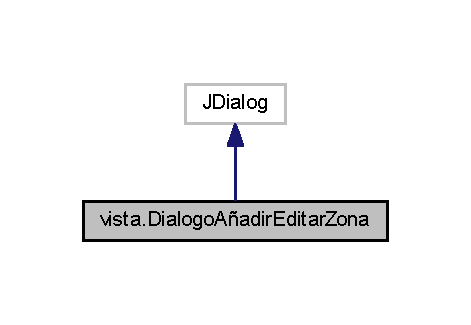
\includegraphics[width=226pt]{classvista_1_1_dialogo_a_xC3_xB1adir_editar_zona__inherit__graph}
\end{center}
\end{figure}


Collaboration diagram for vista.\+Dialogo\+Añadir\+Editar\+Zona\+:
\nopagebreak
\begin{figure}[H]
\begin{center}
\leavevmode
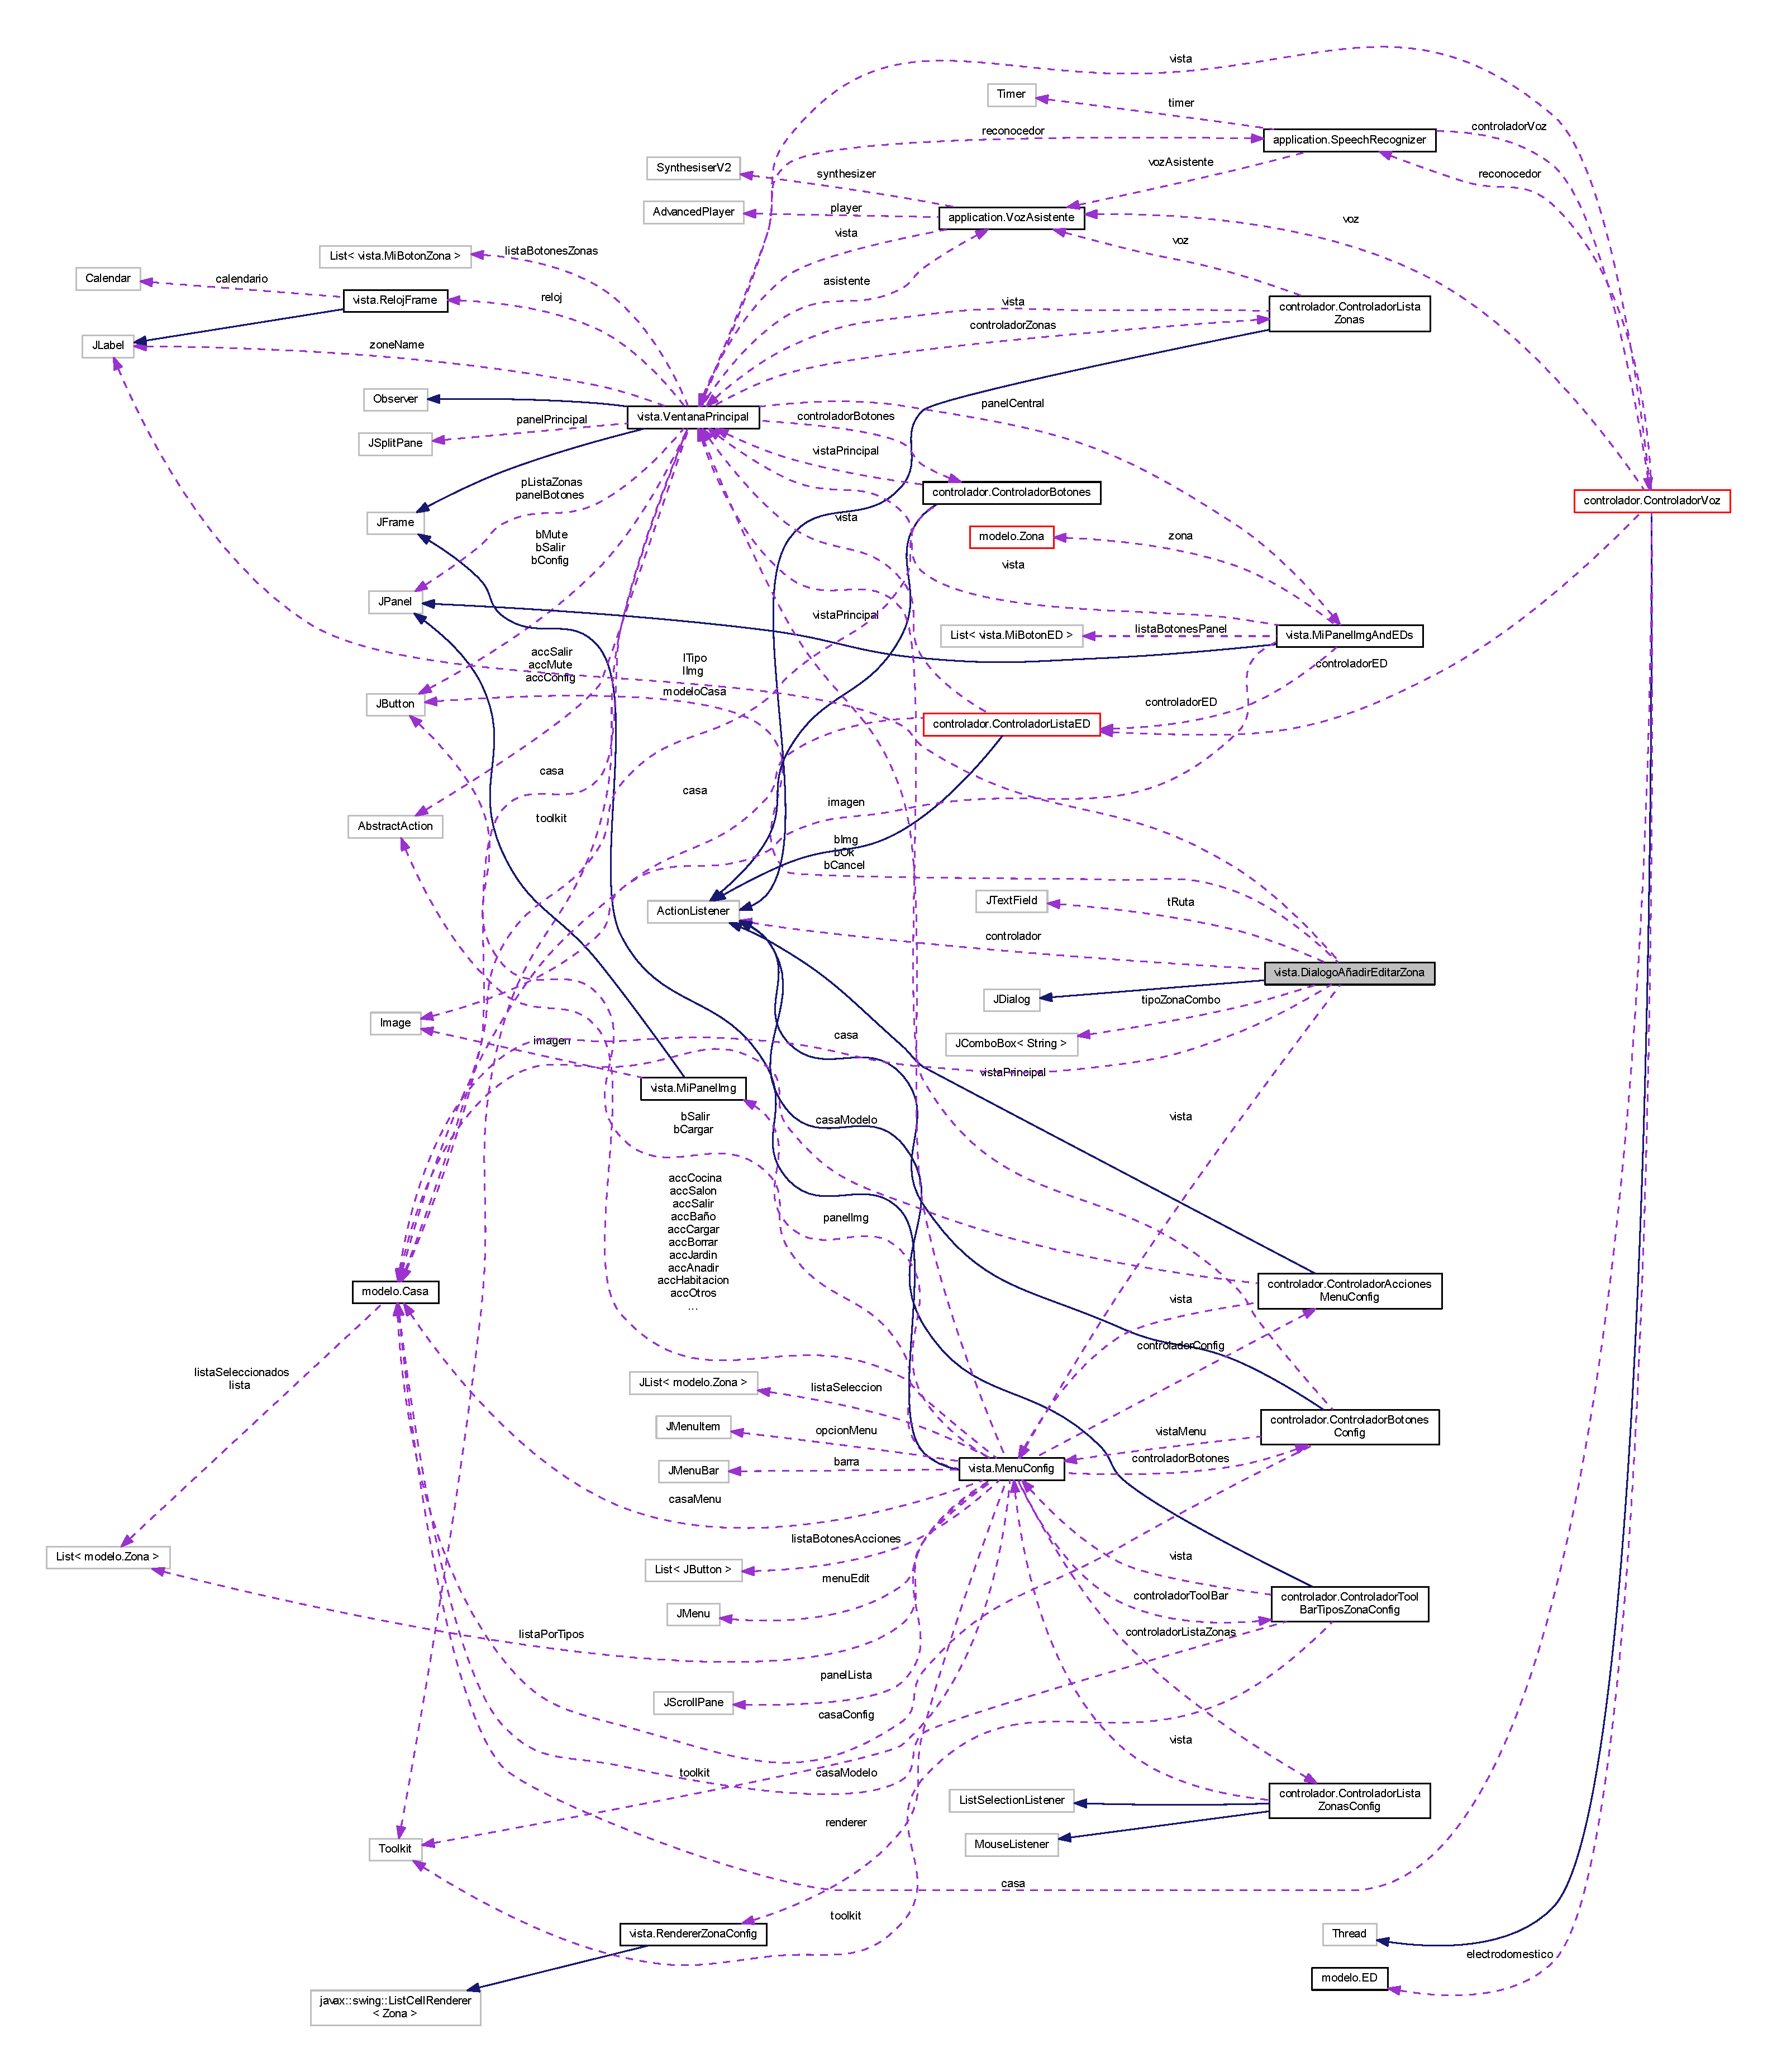
\includegraphics[width=350pt]{classvista_1_1_dialogo_a_xC3_xB1adir_editar_zona__coll__graph}
\end{center}
\end{figure}
\subsection*{Public Member Functions}
\begin{DoxyCompactItemize}
\item 
\mbox{\Hypertarget{classvista_1_1_dialogo_a_xC3_xB1adir_editar_zona_a334c1d2bbdfd703144f614e5b17cd5a7}\label{classvista_1_1_dialogo_a_xC3_xB1adir_editar_zona_a334c1d2bbdfd703144f614e5b17cd5a7}} 
{\bfseries Dialogo\+Añadir\+Editar\+Zona} (J\+Frame ventana, String titulo, boolean modo, boolean esta\+Añadiendo, \mbox{\hyperlink{classmodelo_1_1_casa}{Casa}} casa)
\item 
\mbox{\Hypertarget{classvista_1_1_dialogo_a_xC3_xB1adir_editar_zona_a0d49235e9285853b6cc0a786b7068a3a}\label{classvista_1_1_dialogo_a_xC3_xB1adir_editar_zona_a0d49235e9285853b6cc0a786b7068a3a}} 
J\+Combo\+Box$<$ String $>$ {\bfseries get\+Tipo\+Zona\+Combo} ()
\item 
\mbox{\Hypertarget{classvista_1_1_dialogo_a_xC3_xB1adir_editar_zona_a996c5821e4f9c2abbc6e89be634434a7}\label{classvista_1_1_dialogo_a_xC3_xB1adir_editar_zona_a996c5821e4f9c2abbc6e89be634434a7}} 
J\+List$<$ \mbox{\hyperlink{classmodelo_1_1_zona}{Zona}} $>$ {\bfseries get\+Lista\+Seleccion} ()
\item 
\mbox{\Hypertarget{classvista_1_1_dialogo_a_xC3_xB1adir_editar_zona_ad6de9a76fc2e11bdf48dca18e82f3e81}\label{classvista_1_1_dialogo_a_xC3_xB1adir_editar_zona_ad6de9a76fc2e11bdf48dca18e82f3e81}} 
void {\bfseries add\+Zona\+To\+Casa} (String nombre, String imagen)
\item 
\mbox{\Hypertarget{classvista_1_1_dialogo_a_xC3_xB1adir_editar_zona_a371fa7858769811260180c8774cf73b3}\label{classvista_1_1_dialogo_a_xC3_xB1adir_editar_zona_a371fa7858769811260180c8774cf73b3}} 
void {\bfseries update\+List} ()
\item 
\mbox{\Hypertarget{classvista_1_1_dialogo_a_xC3_xB1adir_editar_zona_a0d9cc9f81e61823751e28641da9834f1}\label{classvista_1_1_dialogo_a_xC3_xB1adir_editar_zona_a0d9cc9f81e61823751e28641da9834f1}} 
\mbox{\hyperlink{classmodelo_1_1_zona}{Zona}} {\bfseries get\+Selected\+Zone} ()
\item 
\mbox{\Hypertarget{classvista_1_1_dialogo_a_xC3_xB1adir_editar_zona_a8916fda5ffd99498a6260218cf310aa2}\label{classvista_1_1_dialogo_a_xC3_xB1adir_editar_zona_a8916fda5ffd99498a6260218cf310aa2}} 
J\+Text\+Field {\bfseries gett\+Ruta} ()
\item 
\mbox{\Hypertarget{classvista_1_1_dialogo_a_xC3_xB1adir_editar_zona_a43768ac16ac5a29ae9c6064065c0cb02}\label{classvista_1_1_dialogo_a_xC3_xB1adir_editar_zona_a43768ac16ac5a29ae9c6064065c0cb02}} 
String {\bfseries get\+Num\+To\+String} (int i)
\end{DoxyCompactItemize}


The documentation for this class was generated from the following file\+:\begin{DoxyCompactItemize}
\item 
C\+:/\+Users/\+Ander/\+Documents/\+Java/\+Dream\+Housev2/src/vista/Dialogo\+Añadir\+Editar\+Zona.\+java\end{DoxyCompactItemize}

\hypertarget{classvista_1_1_dialogo_e_d}{}\section{vista.\+Dialogo\+ED Class Reference}
\label{classvista_1_1_dialogo_e_d}\index{vista.\+Dialogo\+ED@{vista.\+Dialogo\+ED}}


Inheritance diagram for vista.\+Dialogo\+ED\+:
\nopagebreak
\begin{figure}[H]
\begin{center}
\leavevmode
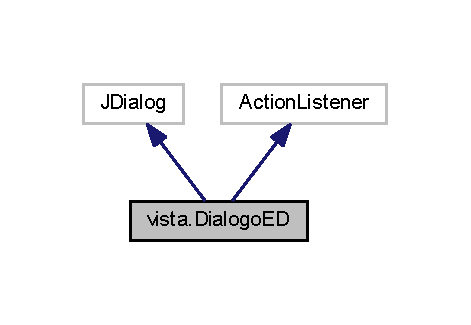
\includegraphics[width=226pt]{classvista_1_1_dialogo_e_d__inherit__graph}
\end{center}
\end{figure}


Collaboration diagram for vista.\+Dialogo\+ED\+:
\nopagebreak
\begin{figure}[H]
\begin{center}
\leavevmode
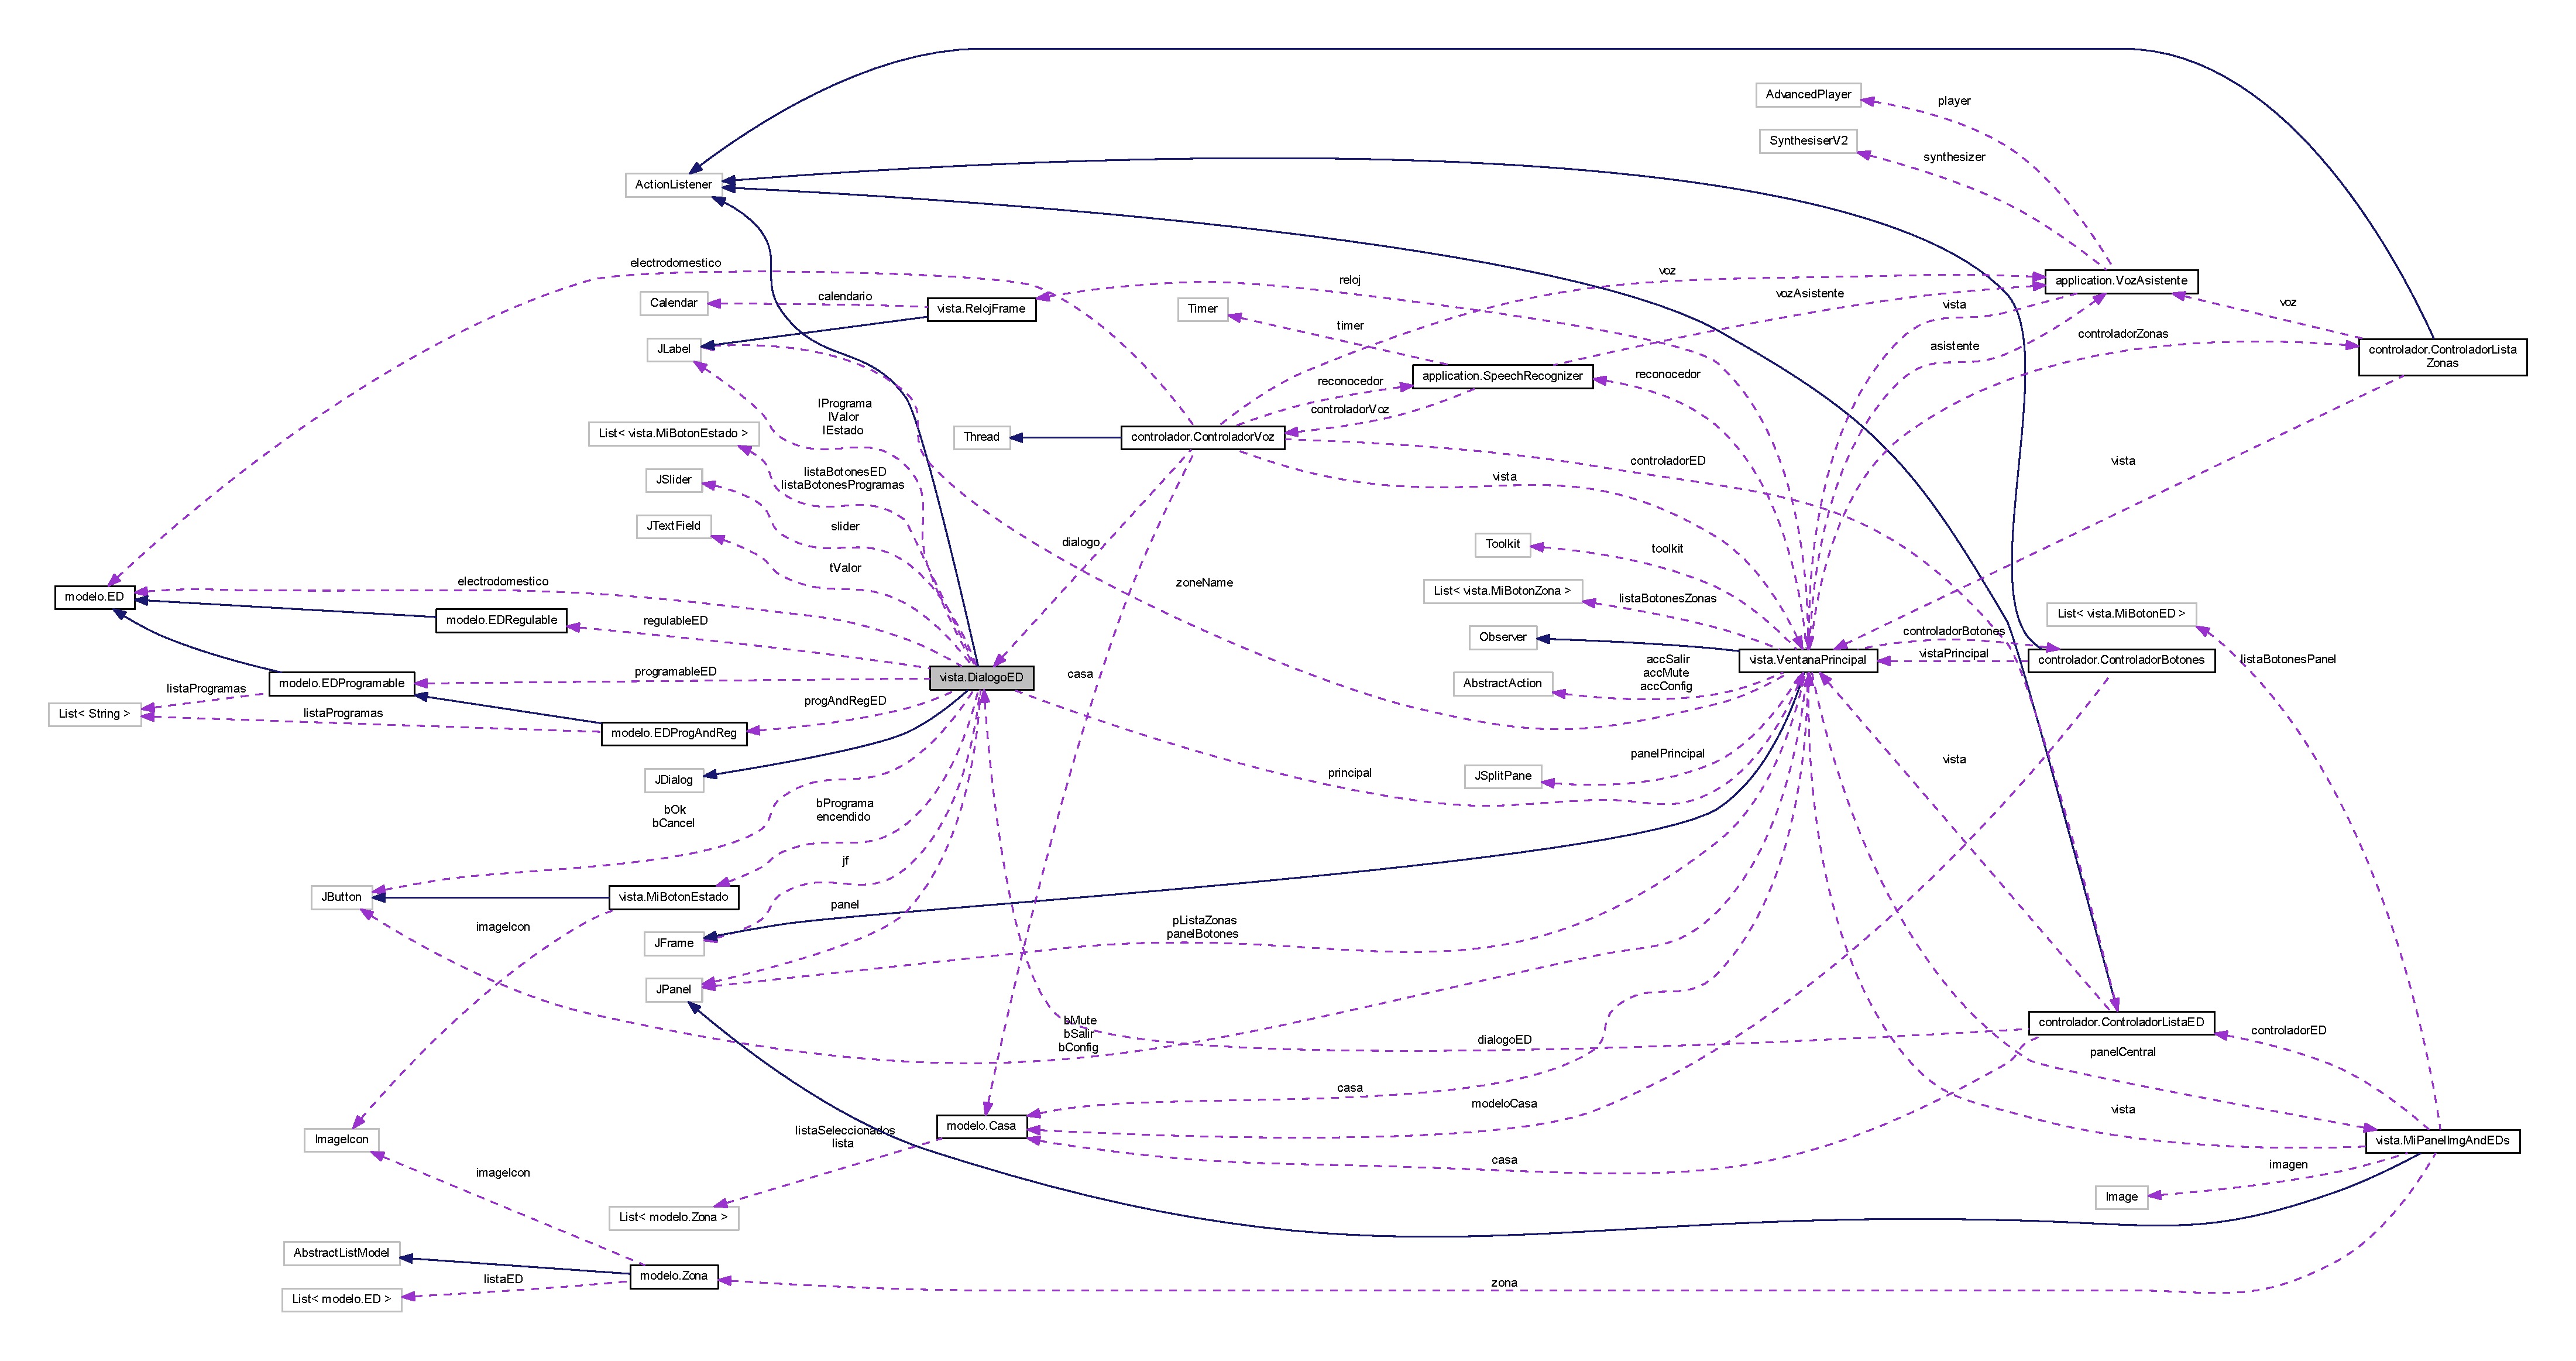
\includegraphics[width=350pt]{classvista_1_1_dialogo_e_d__coll__graph}
\end{center}
\end{figure}
\subsection*{Public Member Functions}
\begin{DoxyCompactItemize}
\item 
\mbox{\Hypertarget{classvista_1_1_dialogo_e_d_a7f7115005d0f3f72df01fdaee9edf904}\label{classvista_1_1_dialogo_e_d_a7f7115005d0f3f72df01fdaee9edf904}} 
{\bfseries Dialogo\+ED} (\mbox{\hyperlink{classvista_1_1_ventana_principal}{Ventana\+Principal}} principal, String nombre, String tipo, \mbox{\hyperlink{classmodelo_1_1_e_d}{ED}} electrodomestico)
\item 
\mbox{\Hypertarget{classvista_1_1_dialogo_e_d_a2cc67426758e03db893c7964c5dc3434}\label{classvista_1_1_dialogo_e_d_a2cc67426758e03db893c7964c5dc3434}} 
J\+Button {\bfseries crear\+Boton} (String nombre)
\item 
\mbox{\Hypertarget{classvista_1_1_dialogo_e_d_ae87e1a5324565d4fd21215a79cbc4249}\label{classvista_1_1_dialogo_e_d_ae87e1a5324565d4fd21215a79cbc4249}} 
\mbox{\hyperlink{classmodelo_1_1_e_d}{ED}} {\bfseries get\+ED} ()
\item 
\mbox{\Hypertarget{classvista_1_1_dialogo_e_d_a3c72cc5cb5d90ccf816f08fe502836a8}\label{classvista_1_1_dialogo_e_d_a3c72cc5cb5d90ccf816f08fe502836a8}} 
void {\bfseries action\+Performed} (Action\+Event e)
\item 
\mbox{\Hypertarget{classvista_1_1_dialogo_e_d_aaad8ad855421519227fe64f578dce276}\label{classvista_1_1_dialogo_e_d_aaad8ad855421519227fe64f578dce276}} 
List$<$ \mbox{\hyperlink{classvista_1_1_mi_boton_estado}{Mi\+Boton\+Estado}} $>$ {\bfseries get\+Lista\+Botones\+ED} ()
\item 
\mbox{\Hypertarget{classvista_1_1_dialogo_e_d_a396d4cbdeee607588ba53cd8ca19fbb0}\label{classvista_1_1_dialogo_e_d_a396d4cbdeee607588ba53cd8ca19fbb0}} 
J\+Slider {\bfseries get\+Slider} ()
\item 
\mbox{\Hypertarget{classvista_1_1_dialogo_e_d_ad56834c0f0dc975064069e162ea99196}\label{classvista_1_1_dialogo_e_d_ad56834c0f0dc975064069e162ea99196}} 
List$<$ J\+Button $>$ {\bfseries get\+Botones\+O\+Ky\+Cancel} ()
\end{DoxyCompactItemize}


The documentation for this class was generated from the following file\+:\begin{DoxyCompactItemize}
\item 
C\+:/\+Users/\+Ander/\+Documents/\+Java/\+Dream\+Housev2/src/vista/Dialogo\+E\+D.\+java\end{DoxyCompactItemize}

\hypertarget{classvista_1_1_dialogo_edit_list_e_d_zona}{}\section{vista.\+Dialogo\+Edit\+List\+E\+D\+Zona Class Reference}
\label{classvista_1_1_dialogo_edit_list_e_d_zona}\index{vista.\+Dialogo\+Edit\+List\+E\+D\+Zona@{vista.\+Dialogo\+Edit\+List\+E\+D\+Zona}}


Inheritance diagram for vista.\+Dialogo\+Edit\+List\+E\+D\+Zona\+:
\nopagebreak
\begin{figure}[H]
\begin{center}
\leavevmode
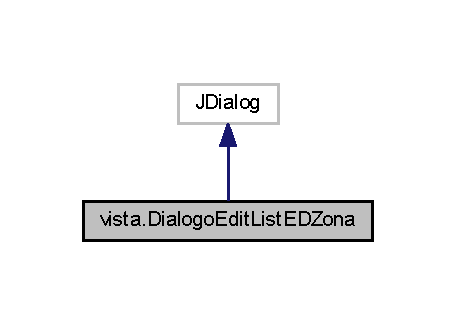
\includegraphics[width=219pt]{classvista_1_1_dialogo_edit_list_e_d_zona__inherit__graph}
\end{center}
\end{figure}


Collaboration diagram for vista.\+Dialogo\+Edit\+List\+E\+D\+Zona\+:
\nopagebreak
\begin{figure}[H]
\begin{center}
\leavevmode
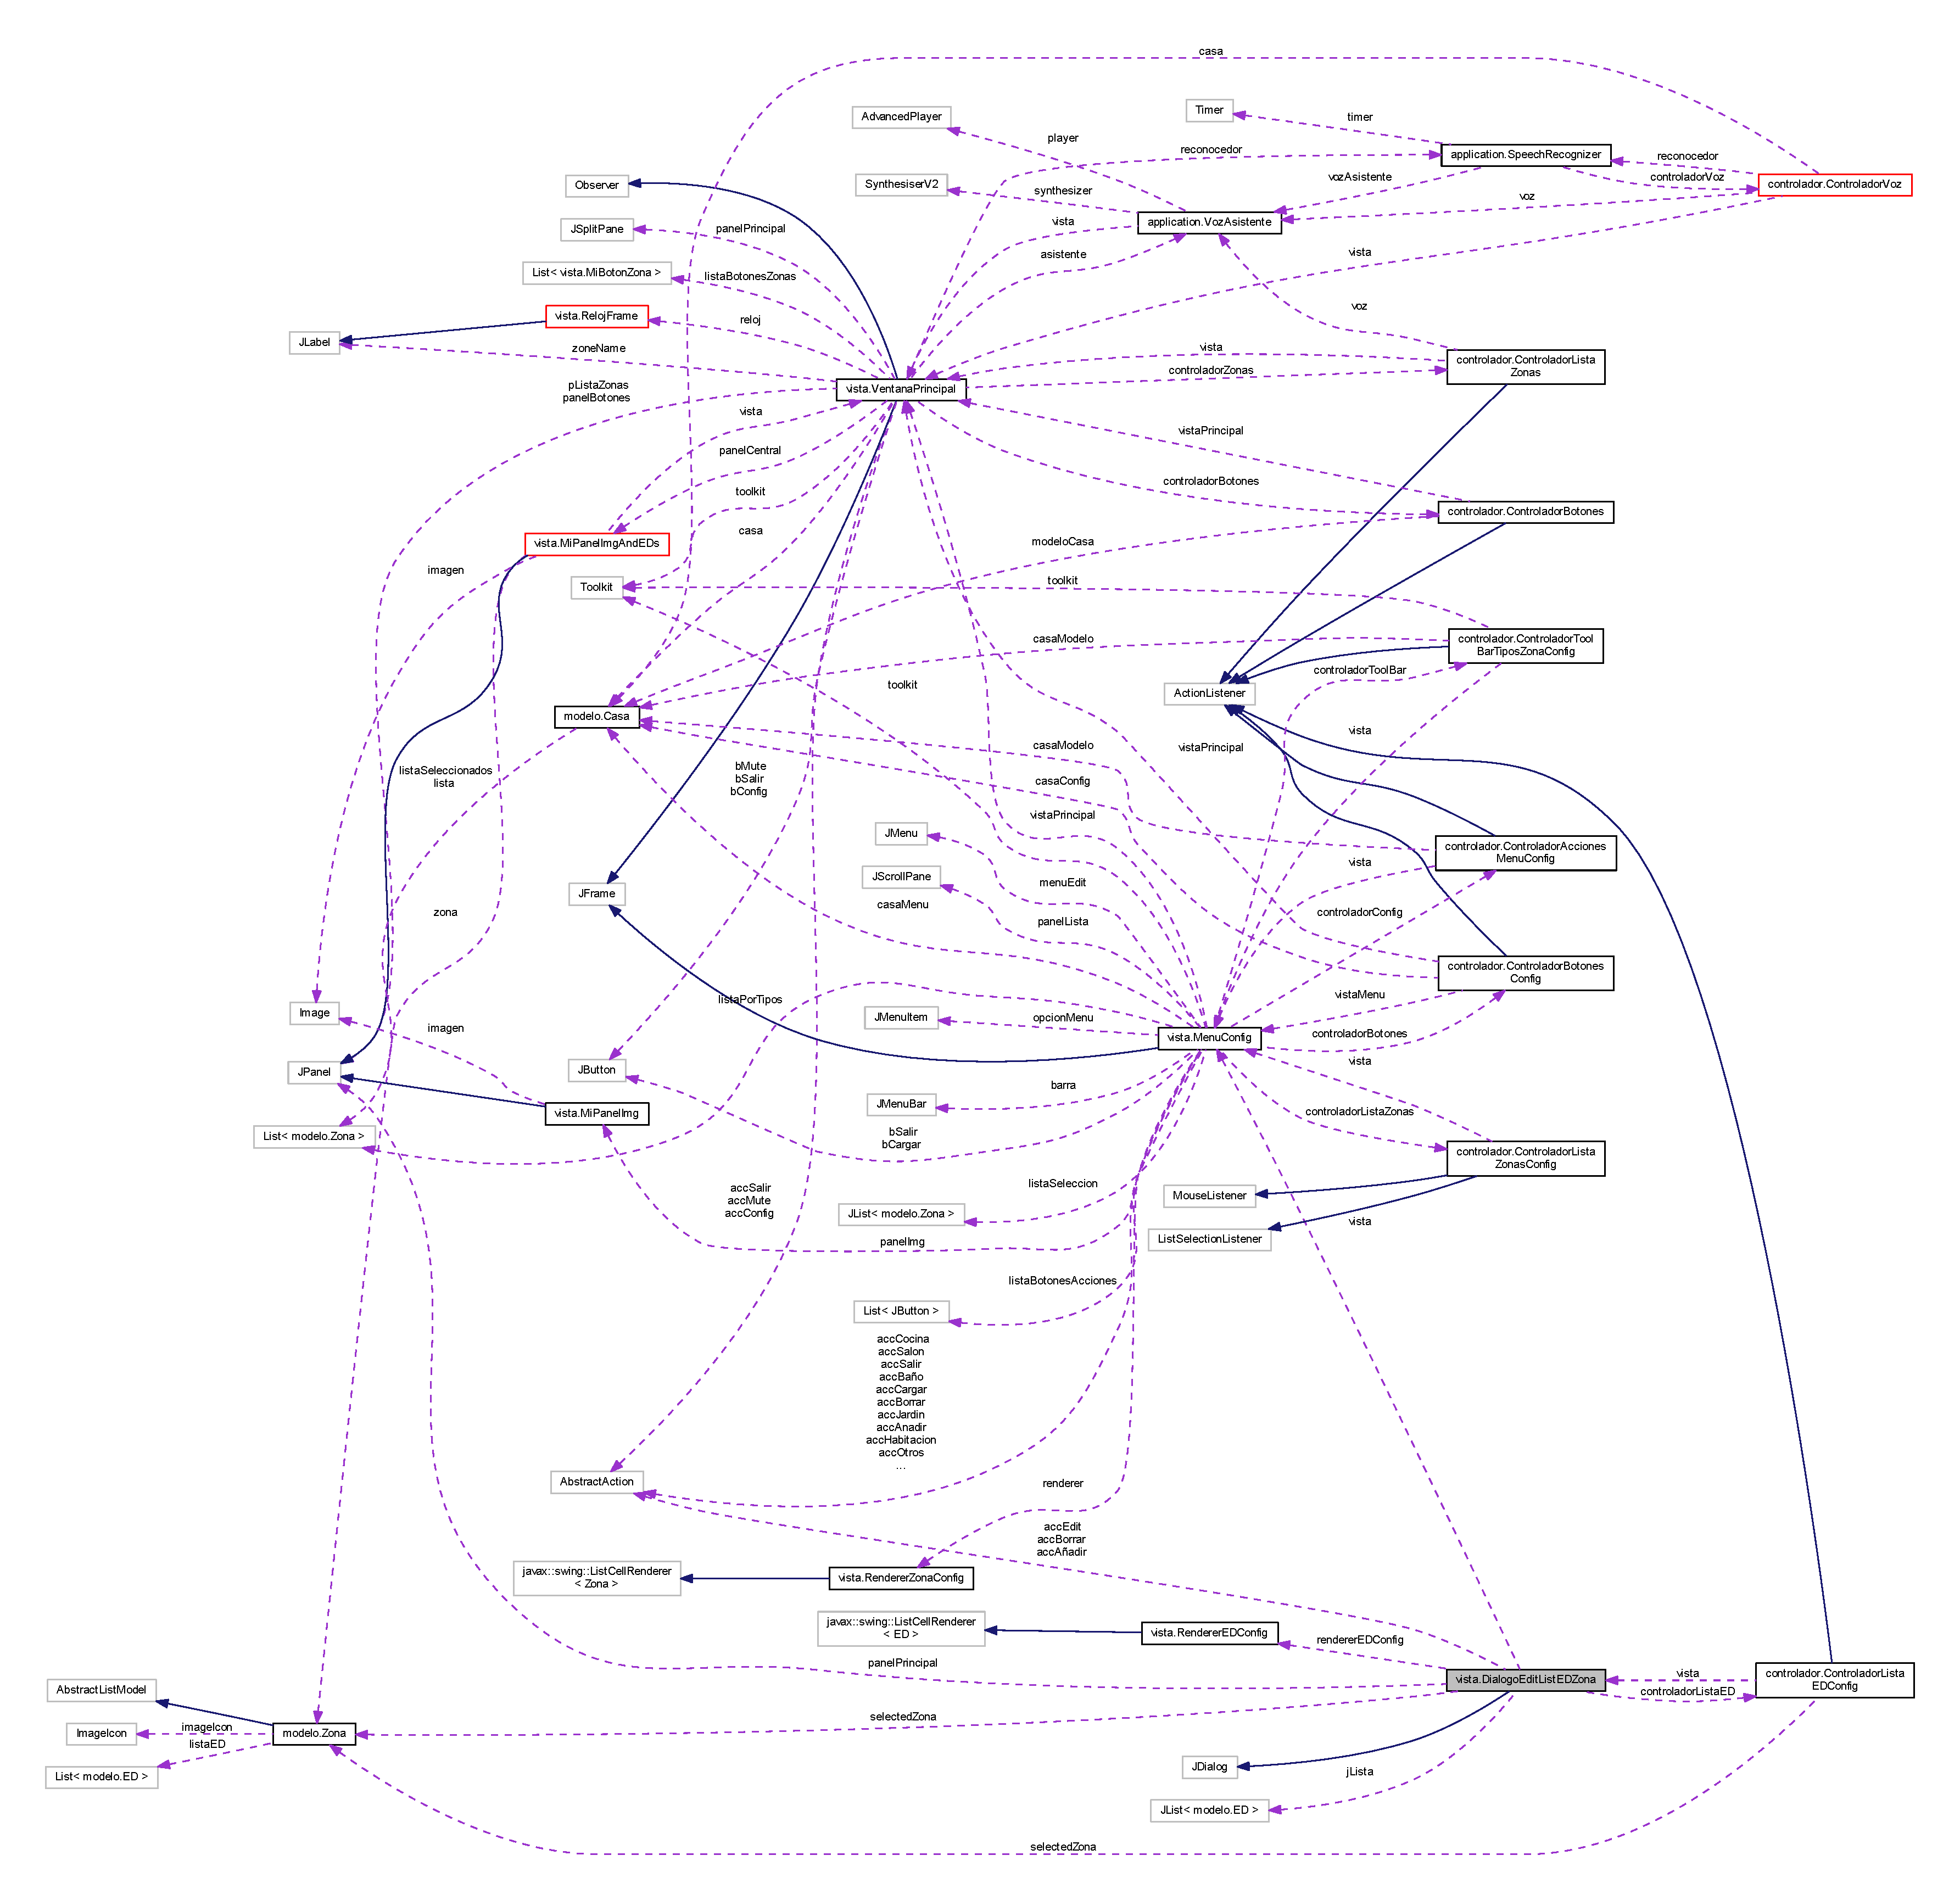
\includegraphics[width=350pt]{classvista_1_1_dialogo_edit_list_e_d_zona__coll__graph}
\end{center}
\end{figure}
\subsection*{Public Member Functions}
\begin{DoxyCompactItemize}
\item 
\mbox{\Hypertarget{classvista_1_1_dialogo_edit_list_e_d_zona_a273305aa9830fb4708b0e5e61ce23d7b}\label{classvista_1_1_dialogo_edit_list_e_d_zona_a273305aa9830fb4708b0e5e61ce23d7b}} 
{\bfseries Dialogo\+Edit\+List\+E\+D\+Zona} (J\+Frame ventana)
\item 
\mbox{\Hypertarget{classvista_1_1_dialogo_edit_list_e_d_zona_a46296f052e9839a3a8c3a8afa7e35fb1}\label{classvista_1_1_dialogo_edit_list_e_d_zona_a46296f052e9839a3a8c3a8afa7e35fb1}} 
\mbox{\hyperlink{classmodelo_1_1_zona}{Zona}} {\bfseries get\+Selected\+Zona} ()
\item 
\mbox{\Hypertarget{classvista_1_1_dialogo_edit_list_e_d_zona_a04493b294406aacc92c5ee9e8fee9351}\label{classvista_1_1_dialogo_edit_list_e_d_zona_a04493b294406aacc92c5ee9e8fee9351}} 
J\+List$<$ \mbox{\hyperlink{classmodelo_1_1_e_d}{ED}} $>$ {\bfseries getj\+Lista} ()
\item 
\mbox{\Hypertarget{classvista_1_1_dialogo_edit_list_e_d_zona_a9ce7cbbde3889d56943a129bec80b538}\label{classvista_1_1_dialogo_edit_list_e_d_zona_a9ce7cbbde3889d56943a129bec80b538}} 
\mbox{\hyperlink{classmodelo_1_1_e_d}{ED}} {\bfseries get\+Selected\+ED} ()
\item 
\mbox{\Hypertarget{classvista_1_1_dialogo_edit_list_e_d_zona_abd21175b4de94d23382219f555e5f6a4}\label{classvista_1_1_dialogo_edit_list_e_d_zona_abd21175b4de94d23382219f555e5f6a4}} 
Abstract\+Action {\bfseries get\+Acc\+Borrar} ()
\item 
\mbox{\Hypertarget{classvista_1_1_dialogo_edit_list_e_d_zona_a50a415351186eb3e9ad68a981f53bd61}\label{classvista_1_1_dialogo_edit_list_e_d_zona_a50a415351186eb3e9ad68a981f53bd61}} 
Abstract\+Action {\bfseries get\+Acc\+Edit} ()
\end{DoxyCompactItemize}


The documentation for this class was generated from the following file\+:\begin{DoxyCompactItemize}
\item 
C\+:/\+Users/\+Ander/\+Documents/\+Java/\+Dream\+Housev2/src/vista/Dialogo\+Edit\+List\+E\+D\+Zona.\+java\end{DoxyCompactItemize}

\hypertarget{classmodelo_1_1_e_d}{}\section{modelo.\+ED Class Reference}
\label{classmodelo_1_1_e_d}\index{modelo.\+ED@{modelo.\+ED}}


Inheritance diagram for modelo.\+ED\+:
\nopagebreak
\begin{figure}[H]
\begin{center}
\leavevmode
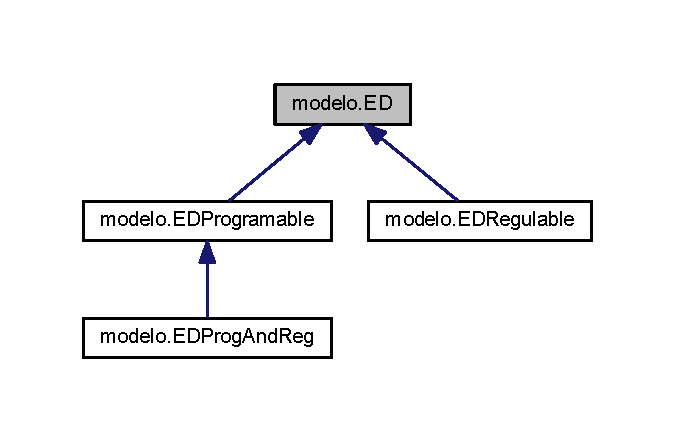
\includegraphics[width=324pt]{classmodelo_1_1_e_d__inherit__graph}
\end{center}
\end{figure}
\subsection*{Public Member Functions}
\begin{DoxyCompactItemize}
\item 
\mbox{\Hypertarget{classmodelo_1_1_e_d_ad95b8183b75d33d1e69555041e595262}\label{classmodelo_1_1_e_d_ad95b8183b75d33d1e69555041e595262}} 
{\bfseries ED} (String n, String img, boolean estado)
\item 
\mbox{\Hypertarget{classmodelo_1_1_e_d_a4a78274dca0082f34ea7c03bb8b34bdd}\label{classmodelo_1_1_e_d_a4a78274dca0082f34ea7c03bb8b34bdd}} 
{\bfseries ED} (String linea)
\item 
\mbox{\Hypertarget{classmodelo_1_1_e_d_a3a831edc54f3b1d9451ad9358e18c63b}\label{classmodelo_1_1_e_d_a3a831edc54f3b1d9451ad9358e18c63b}} 
int {\bfseries get\+I\+Dde\+Nombre} ()
\item 
\mbox{\Hypertarget{classmodelo_1_1_e_d_a5544596d88811fba6207e688d862d675}\label{classmodelo_1_1_e_d_a5544596d88811fba6207e688d862d675}} 
String {\bfseries get\+Tipo\+ED} ()
\item 
\mbox{\Hypertarget{classmodelo_1_1_e_d_a56fdd989da6d3ae993efbd8732dea073}\label{classmodelo_1_1_e_d_a56fdd989da6d3ae993efbd8732dea073}} 
void {\bfseries switch\+Status} ()
\item 
\mbox{\Hypertarget{classmodelo_1_1_e_d_a4ff6ff8bd69e9d8a18cc93c544648ea7}\label{classmodelo_1_1_e_d_a4ff6ff8bd69e9d8a18cc93c544648ea7}} 
String {\bfseries get\+Nombre} ()
\item 
\mbox{\Hypertarget{classmodelo_1_1_e_d_a88e344ca2fceda1e27d2d7c373dc0b61}\label{classmodelo_1_1_e_d_a88e344ca2fceda1e27d2d7c373dc0b61}} 
String {\bfseries get\+Imagen} ()
\item 
\mbox{\Hypertarget{classmodelo_1_1_e_d_a5650f97fda341ffe61c2a5f86865540e}\label{classmodelo_1_1_e_d_a5650f97fda341ffe61c2a5f86865540e}} 
void {\bfseries set\+Nombre} (String nombre)
\item 
\mbox{\Hypertarget{classmodelo_1_1_e_d_a69fdfb590fdb2bca589aace8c760922d}\label{classmodelo_1_1_e_d_a69fdfb590fdb2bca589aace8c760922d}} 
boolean {\bfseries is\+Selected} ()
\item 
\mbox{\Hypertarget{classmodelo_1_1_e_d_af5f19608ff75e1e2598720d53f78d020}\label{classmodelo_1_1_e_d_af5f19608ff75e1e2598720d53f78d020}} 
void {\bfseries switch\+Is\+Selected} ()
\item 
\mbox{\Hypertarget{classmodelo_1_1_e_d_a0c76a786c73a3f35dda3126adcb96c67}\label{classmodelo_1_1_e_d_a0c76a786c73a3f35dda3126adcb96c67}} 
void {\bfseries set\+Selected} (boolean is\+Selected)
\item 
\mbox{\Hypertarget{classmodelo_1_1_e_d_aadb07ef1218bda2ede87c34610084c35}\label{classmodelo_1_1_e_d_aadb07ef1218bda2ede87c34610084c35}} 
boolean {\bfseries get\+Estado} ()
\item 
\mbox{\Hypertarget{classmodelo_1_1_e_d_af6910c0fb0772f5467f2957737903342}\label{classmodelo_1_1_e_d_af6910c0fb0772f5467f2957737903342}} 
void {\bfseries cambiar\+Estado} ()
\item 
\mbox{\Hypertarget{classmodelo_1_1_e_d_ad4534d695019f9baaf841ce40dc58338}\label{classmodelo_1_1_e_d_ad4534d695019f9baaf841ce40dc58338}} 
void {\bfseries set\+Estado} (boolean estado)
\item 
\mbox{\Hypertarget{classmodelo_1_1_e_d_ad81faa7b79bdc75f0952cba078266b1e}\label{classmodelo_1_1_e_d_ad81faa7b79bdc75f0952cba078266b1e}} 
String {\bfseries to\+String\+File} ()
\item 
\mbox{\Hypertarget{classmodelo_1_1_e_d_a299fd5ea8b36c66271e0cd99e5f7f7a1}\label{classmodelo_1_1_e_d_a299fd5ea8b36c66271e0cd99e5f7f7a1}} 
String {\bfseries to\+String} ()
\end{DoxyCompactItemize}


The documentation for this class was generated from the following file\+:\begin{DoxyCompactItemize}
\item 
C\+:/\+Users/\+Ander/\+Documents/\+Java/\+Dream\+Housev2/src/modelo/E\+D.\+java\end{DoxyCompactItemize}

\hypertarget{classmodelo_1_1_e_d_prog_and_reg}{}\section{modelo.\+E\+D\+Prog\+And\+Reg Class Reference}
\label{classmodelo_1_1_e_d_prog_and_reg}\index{modelo.\+E\+D\+Prog\+And\+Reg@{modelo.\+E\+D\+Prog\+And\+Reg}}


Inheritance diagram for modelo.\+E\+D\+Prog\+And\+Reg\+:
\nopagebreak
\begin{figure}[H]
\begin{center}
\leavevmode
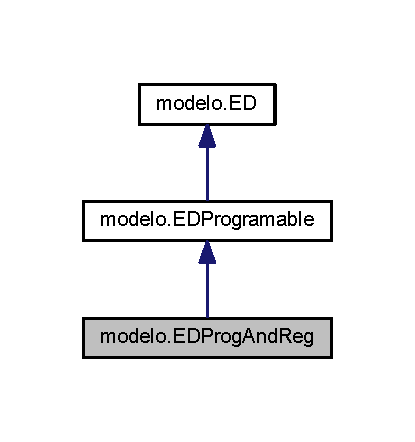
\includegraphics[width=199pt]{classmodelo_1_1_e_d_prog_and_reg__inherit__graph}
\end{center}
\end{figure}


Collaboration diagram for modelo.\+E\+D\+Prog\+And\+Reg\+:
\nopagebreak
\begin{figure}[H]
\begin{center}
\leavevmode
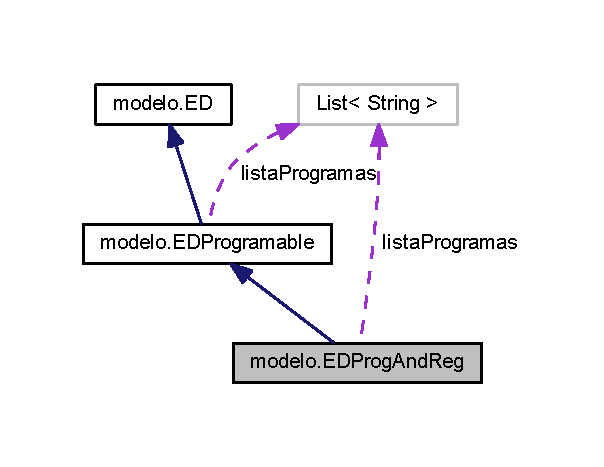
\includegraphics[width=290pt]{classmodelo_1_1_e_d_prog_and_reg__coll__graph}
\end{center}
\end{figure}
\subsection*{Public Member Functions}
\begin{DoxyCompactItemize}
\item 
\mbox{\Hypertarget{classmodelo_1_1_e_d_prog_and_reg_a59fd32988f0e7886544d49601d554d11}\label{classmodelo_1_1_e_d_prog_and_reg_a59fd32988f0e7886544d49601d554d11}} 
{\bfseries E\+D\+Prog\+And\+Reg} (String n, String img, boolean estado, int v\+Min, int v\+Max, int valor, String programa, List$<$ String $>$ lista)
\item 
\mbox{\Hypertarget{classmodelo_1_1_e_d_prog_and_reg_a0c934bb38fa4acafb27014c962966c86}\label{classmodelo_1_1_e_d_prog_and_reg_a0c934bb38fa4acafb27014c962966c86}} 
{\bfseries E\+D\+Prog\+And\+Reg} (String linea)
\item 
\mbox{\Hypertarget{classmodelo_1_1_e_d_prog_and_reg_a357c68f3e389b1b7be1d0991ca1af7f4}\label{classmodelo_1_1_e_d_prog_and_reg_a357c68f3e389b1b7be1d0991ca1af7f4}} 
int {\bfseries get\+Valor} ()
\item 
\mbox{\Hypertarget{classmodelo_1_1_e_d_prog_and_reg_a1f67e7a977bd3c7ed6a551f103dda7b2}\label{classmodelo_1_1_e_d_prog_and_reg_a1f67e7a977bd3c7ed6a551f103dda7b2}} 
int {\bfseries getv\+Min} ()
\item 
\mbox{\Hypertarget{classmodelo_1_1_e_d_prog_and_reg_a606f1c6e59684cf36e9e232f1c8c74b5}\label{classmodelo_1_1_e_d_prog_and_reg_a606f1c6e59684cf36e9e232f1c8c74b5}} 
int {\bfseries getv\+Max} ()
\item 
\mbox{\Hypertarget{classmodelo_1_1_e_d_prog_and_reg_acd217e74e210b80ab0ae9028d8d2e238}\label{classmodelo_1_1_e_d_prog_and_reg_acd217e74e210b80ab0ae9028d8d2e238}} 
void {\bfseries set\+Valor} (int valor)
\item 
\mbox{\Hypertarget{classmodelo_1_1_e_d_prog_and_reg_a9bb036d2596a73b2af9a9959ad564b31}\label{classmodelo_1_1_e_d_prog_and_reg_a9bb036d2596a73b2af9a9959ad564b31}} 
String {\bfseries to\+String\+File} ()
\item 
\mbox{\Hypertarget{classmodelo_1_1_e_d_prog_and_reg_a7f61e2cc66f9d7adb21d0829e6b49d06}\label{classmodelo_1_1_e_d_prog_and_reg_a7f61e2cc66f9d7adb21d0829e6b49d06}} 
String {\bfseries to\+String} ()
\end{DoxyCompactItemize}


The documentation for this class was generated from the following file\+:\begin{DoxyCompactItemize}
\item 
C\+:/\+Users/\+Ander/\+Documents/\+Java/\+Dream\+Housev2/src/modelo/E\+D\+Prog\+And\+Reg.\+java\end{DoxyCompactItemize}

\hypertarget{classmodelo_1_1_e_d_programable}{}\section{modelo.\+E\+D\+Programable Class Reference}
\label{classmodelo_1_1_e_d_programable}\index{modelo.\+E\+D\+Programable@{modelo.\+E\+D\+Programable}}


Inheritance diagram for modelo.\+E\+D\+Programable\+:
\nopagebreak
\begin{figure}[H]
\begin{center}
\leavevmode
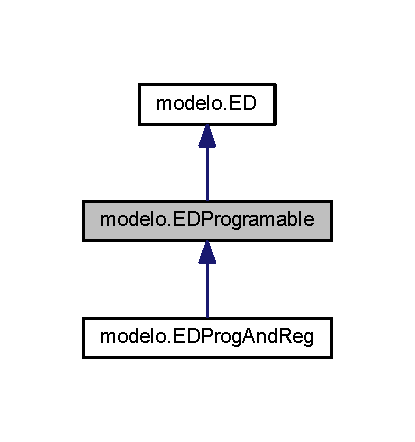
\includegraphics[width=199pt]{classmodelo_1_1_e_d_programable__inherit__graph}
\end{center}
\end{figure}


Collaboration diagram for modelo.\+E\+D\+Programable\+:
\nopagebreak
\begin{figure}[H]
\begin{center}
\leavevmode
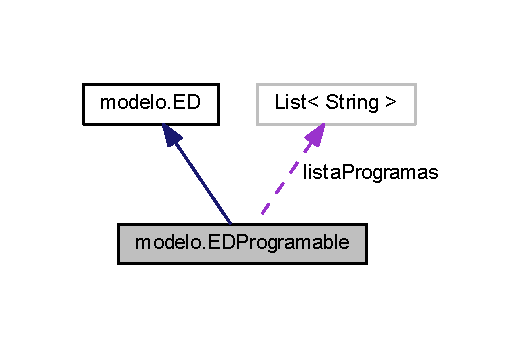
\includegraphics[width=252pt]{classmodelo_1_1_e_d_programable__coll__graph}
\end{center}
\end{figure}
\subsection*{Public Member Functions}
\begin{DoxyCompactItemize}
\item 
\mbox{\Hypertarget{classmodelo_1_1_e_d_programable_acdbaee3588ae86f0b3846174a3315f7f}\label{classmodelo_1_1_e_d_programable_acdbaee3588ae86f0b3846174a3315f7f}} 
{\bfseries E\+D\+Programable} (String n, String img, boolean estado, String programa, List$<$ String $>$ lista)
\item 
\mbox{\Hypertarget{classmodelo_1_1_e_d_programable_a83fc76bd8e7b38da1eaca4adf090bc51}\label{classmodelo_1_1_e_d_programable_a83fc76bd8e7b38da1eaca4adf090bc51}} 
String {\bfseries get\+Programa} ()
\item 
\mbox{\Hypertarget{classmodelo_1_1_e_d_programable_a17f43d67346fc47216adb631225ca70b}\label{classmodelo_1_1_e_d_programable_a17f43d67346fc47216adb631225ca70b}} 
void {\bfseries set\+Programa} (String programa)
\item 
\mbox{\Hypertarget{classmodelo_1_1_e_d_programable_a4831d2cbeb888123f271c6703d50a3d0}\label{classmodelo_1_1_e_d_programable_a4831d2cbeb888123f271c6703d50a3d0}} 
List$<$ String $>$ {\bfseries get\+Lista\+Programas} ()
\item 
\mbox{\Hypertarget{classmodelo_1_1_e_d_programable_ad7b55ad5c04fd084089e5d794ed65454}\label{classmodelo_1_1_e_d_programable_ad7b55ad5c04fd084089e5d794ed65454}} 
{\bfseries E\+D\+Programable} (String linea)
\item 
\mbox{\Hypertarget{classmodelo_1_1_e_d_programable_aa12df54712ea2dfc73fbb89da595ca11}\label{classmodelo_1_1_e_d_programable_aa12df54712ea2dfc73fbb89da595ca11}} 
List$<$ String $>$ {\bfseries get\+Lista} ()
\item 
\mbox{\Hypertarget{classmodelo_1_1_e_d_programable_afc84581d73aaf75bd833fe029a5d6f33}\label{classmodelo_1_1_e_d_programable_afc84581d73aaf75bd833fe029a5d6f33}} 
String {\bfseries to\+String} ()
\item 
\mbox{\Hypertarget{classmodelo_1_1_e_d_programable_a73931112f3e7effc39bed0223efaa428}\label{classmodelo_1_1_e_d_programable_a73931112f3e7effc39bed0223efaa428}} 
String {\bfseries to\+String\+File} ()
\end{DoxyCompactItemize}


The documentation for this class was generated from the following file\+:\begin{DoxyCompactItemize}
\item 
C\+:/\+Users/\+Ander/\+Documents/\+Java/\+Dream\+Housev2/src/modelo/E\+D\+Programable.\+java\end{DoxyCompactItemize}

\hypertarget{classmodelo_1_1_e_d_regulable}{}\section{modelo.\+E\+D\+Regulable Class Reference}
\label{classmodelo_1_1_e_d_regulable}\index{modelo.\+E\+D\+Regulable@{modelo.\+E\+D\+Regulable}}


Inheritance diagram for modelo.\+E\+D\+Regulable\+:
\nopagebreak
\begin{figure}[H]
\begin{center}
\leavevmode
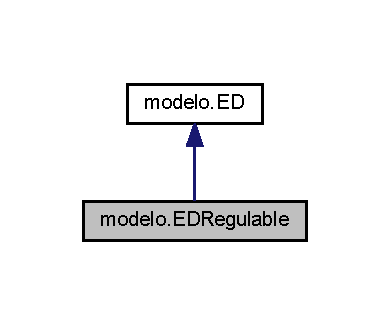
\includegraphics[width=187pt]{classmodelo_1_1_e_d_regulable__inherit__graph}
\end{center}
\end{figure}


Collaboration diagram for modelo.\+E\+D\+Regulable\+:
\nopagebreak
\begin{figure}[H]
\begin{center}
\leavevmode
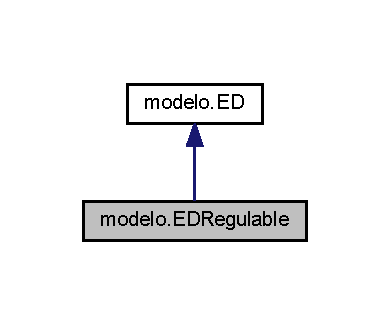
\includegraphics[width=187pt]{classmodelo_1_1_e_d_regulable__coll__graph}
\end{center}
\end{figure}
\subsection*{Public Member Functions}
\begin{DoxyCompactItemize}
\item 
\mbox{\Hypertarget{classmodelo_1_1_e_d_regulable_aa269c52c783882ba76f21807dba145d7}\label{classmodelo_1_1_e_d_regulable_aa269c52c783882ba76f21807dba145d7}} 
{\bfseries E\+D\+Regulable} (String n, String img, boolean estado, int v\+Min, int v\+Max, int valor)
\item 
\mbox{\Hypertarget{classmodelo_1_1_e_d_regulable_a1cd8aedd21851c563533c41a7f093b89}\label{classmodelo_1_1_e_d_regulable_a1cd8aedd21851c563533c41a7f093b89}} 
int {\bfseries getv\+Max} ()
\item 
\mbox{\Hypertarget{classmodelo_1_1_e_d_regulable_a92f95c7d268e4c0c8f400822acff96e9}\label{classmodelo_1_1_e_d_regulable_a92f95c7d268e4c0c8f400822acff96e9}} 
void {\bfseries setv\+Max} (int v\+Max)
\item 
\mbox{\Hypertarget{classmodelo_1_1_e_d_regulable_a29ff167bb69c6cdd44964d8a9703d098}\label{classmodelo_1_1_e_d_regulable_a29ff167bb69c6cdd44964d8a9703d098}} 
int {\bfseries getv\+Min} ()
\item 
\mbox{\Hypertarget{classmodelo_1_1_e_d_regulable_a9b665b5cb50aa079f2c3ecde2101a96a}\label{classmodelo_1_1_e_d_regulable_a9b665b5cb50aa079f2c3ecde2101a96a}} 
void {\bfseries setv\+Min} (int v\+Min)
\item 
\mbox{\Hypertarget{classmodelo_1_1_e_d_regulable_a1d6a61d20c823c5bd383b0e4e841644e}\label{classmodelo_1_1_e_d_regulable_a1d6a61d20c823c5bd383b0e4e841644e}} 
int {\bfseries get\+Valor} ()
\item 
\mbox{\Hypertarget{classmodelo_1_1_e_d_regulable_ad34348929673372480fe4f0e7fc50305}\label{classmodelo_1_1_e_d_regulable_ad34348929673372480fe4f0e7fc50305}} 
void {\bfseries set\+Valor} (int valor)
\item 
\mbox{\Hypertarget{classmodelo_1_1_e_d_regulable_a9e9ad99f51d31c38bf7c0a1bdb826ee4}\label{classmodelo_1_1_e_d_regulable_a9e9ad99f51d31c38bf7c0a1bdb826ee4}} 
{\bfseries E\+D\+Regulable} (String linea)
\item 
\mbox{\Hypertarget{classmodelo_1_1_e_d_regulable_a99c9d9c305eab98d121ba917a042ae3e}\label{classmodelo_1_1_e_d_regulable_a99c9d9c305eab98d121ba917a042ae3e}} 
String {\bfseries to\+String\+File} ()
\item 
\mbox{\Hypertarget{classmodelo_1_1_e_d_regulable_a5802caa573177c48bda77ae4d9e487a9}\label{classmodelo_1_1_e_d_regulable_a5802caa573177c48bda77ae4d9e487a9}} 
String {\bfseries to\+String} ()
\end{DoxyCompactItemize}


The documentation for this class was generated from the following file\+:\begin{DoxyCompactItemize}
\item 
C\+:/\+Users/\+Ander/\+Documents/\+Java/\+Dream\+Housev2/src/modelo/E\+D\+Regulable.\+java\end{DoxyCompactItemize}

\hypertarget{classvista_1_1_logo}{}\section{vista.\+Logo Class Reference}
\label{classvista_1_1_logo}\index{vista.\+Logo@{vista.\+Logo}}


Inheritance diagram for vista.\+Logo\+:
\nopagebreak
\begin{figure}[H]
\begin{center}
\leavevmode
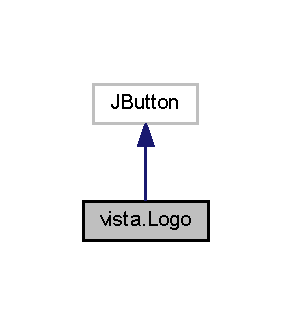
\includegraphics[width=140pt]{classvista_1_1_logo__inherit__graph}
\end{center}
\end{figure}


Collaboration diagram for vista.\+Logo\+:
\nopagebreak
\begin{figure}[H]
\begin{center}
\leavevmode
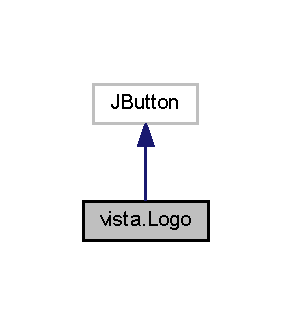
\includegraphics[width=140pt]{classvista_1_1_logo__coll__graph}
\end{center}
\end{figure}


The documentation for this class was generated from the following file\+:\begin{DoxyCompactItemize}
\item 
C\+:/\+Users/\+Ander/\+Documents/\+Java/\+Dream\+Housev2/src/vista/Logo.\+java\end{DoxyCompactItemize}

\hypertarget{classvista_1_1_menu_config}{}\section{vista.\+Menu\+Config Class Reference}
\label{classvista_1_1_menu_config}\index{vista.\+Menu\+Config@{vista.\+Menu\+Config}}


Inheritance diagram for vista.\+Menu\+Config\+:
\nopagebreak
\begin{figure}[H]
\begin{center}
\leavevmode
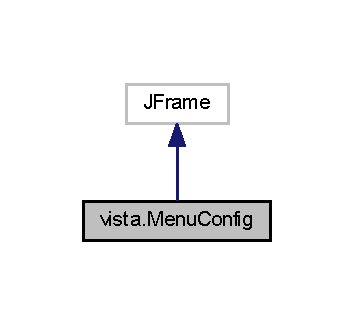
\includegraphics[width=170pt]{classvista_1_1_menu_config__inherit__graph}
\end{center}
\end{figure}


Collaboration diagram for vista.\+Menu\+Config\+:
\nopagebreak
\begin{figure}[H]
\begin{center}
\leavevmode
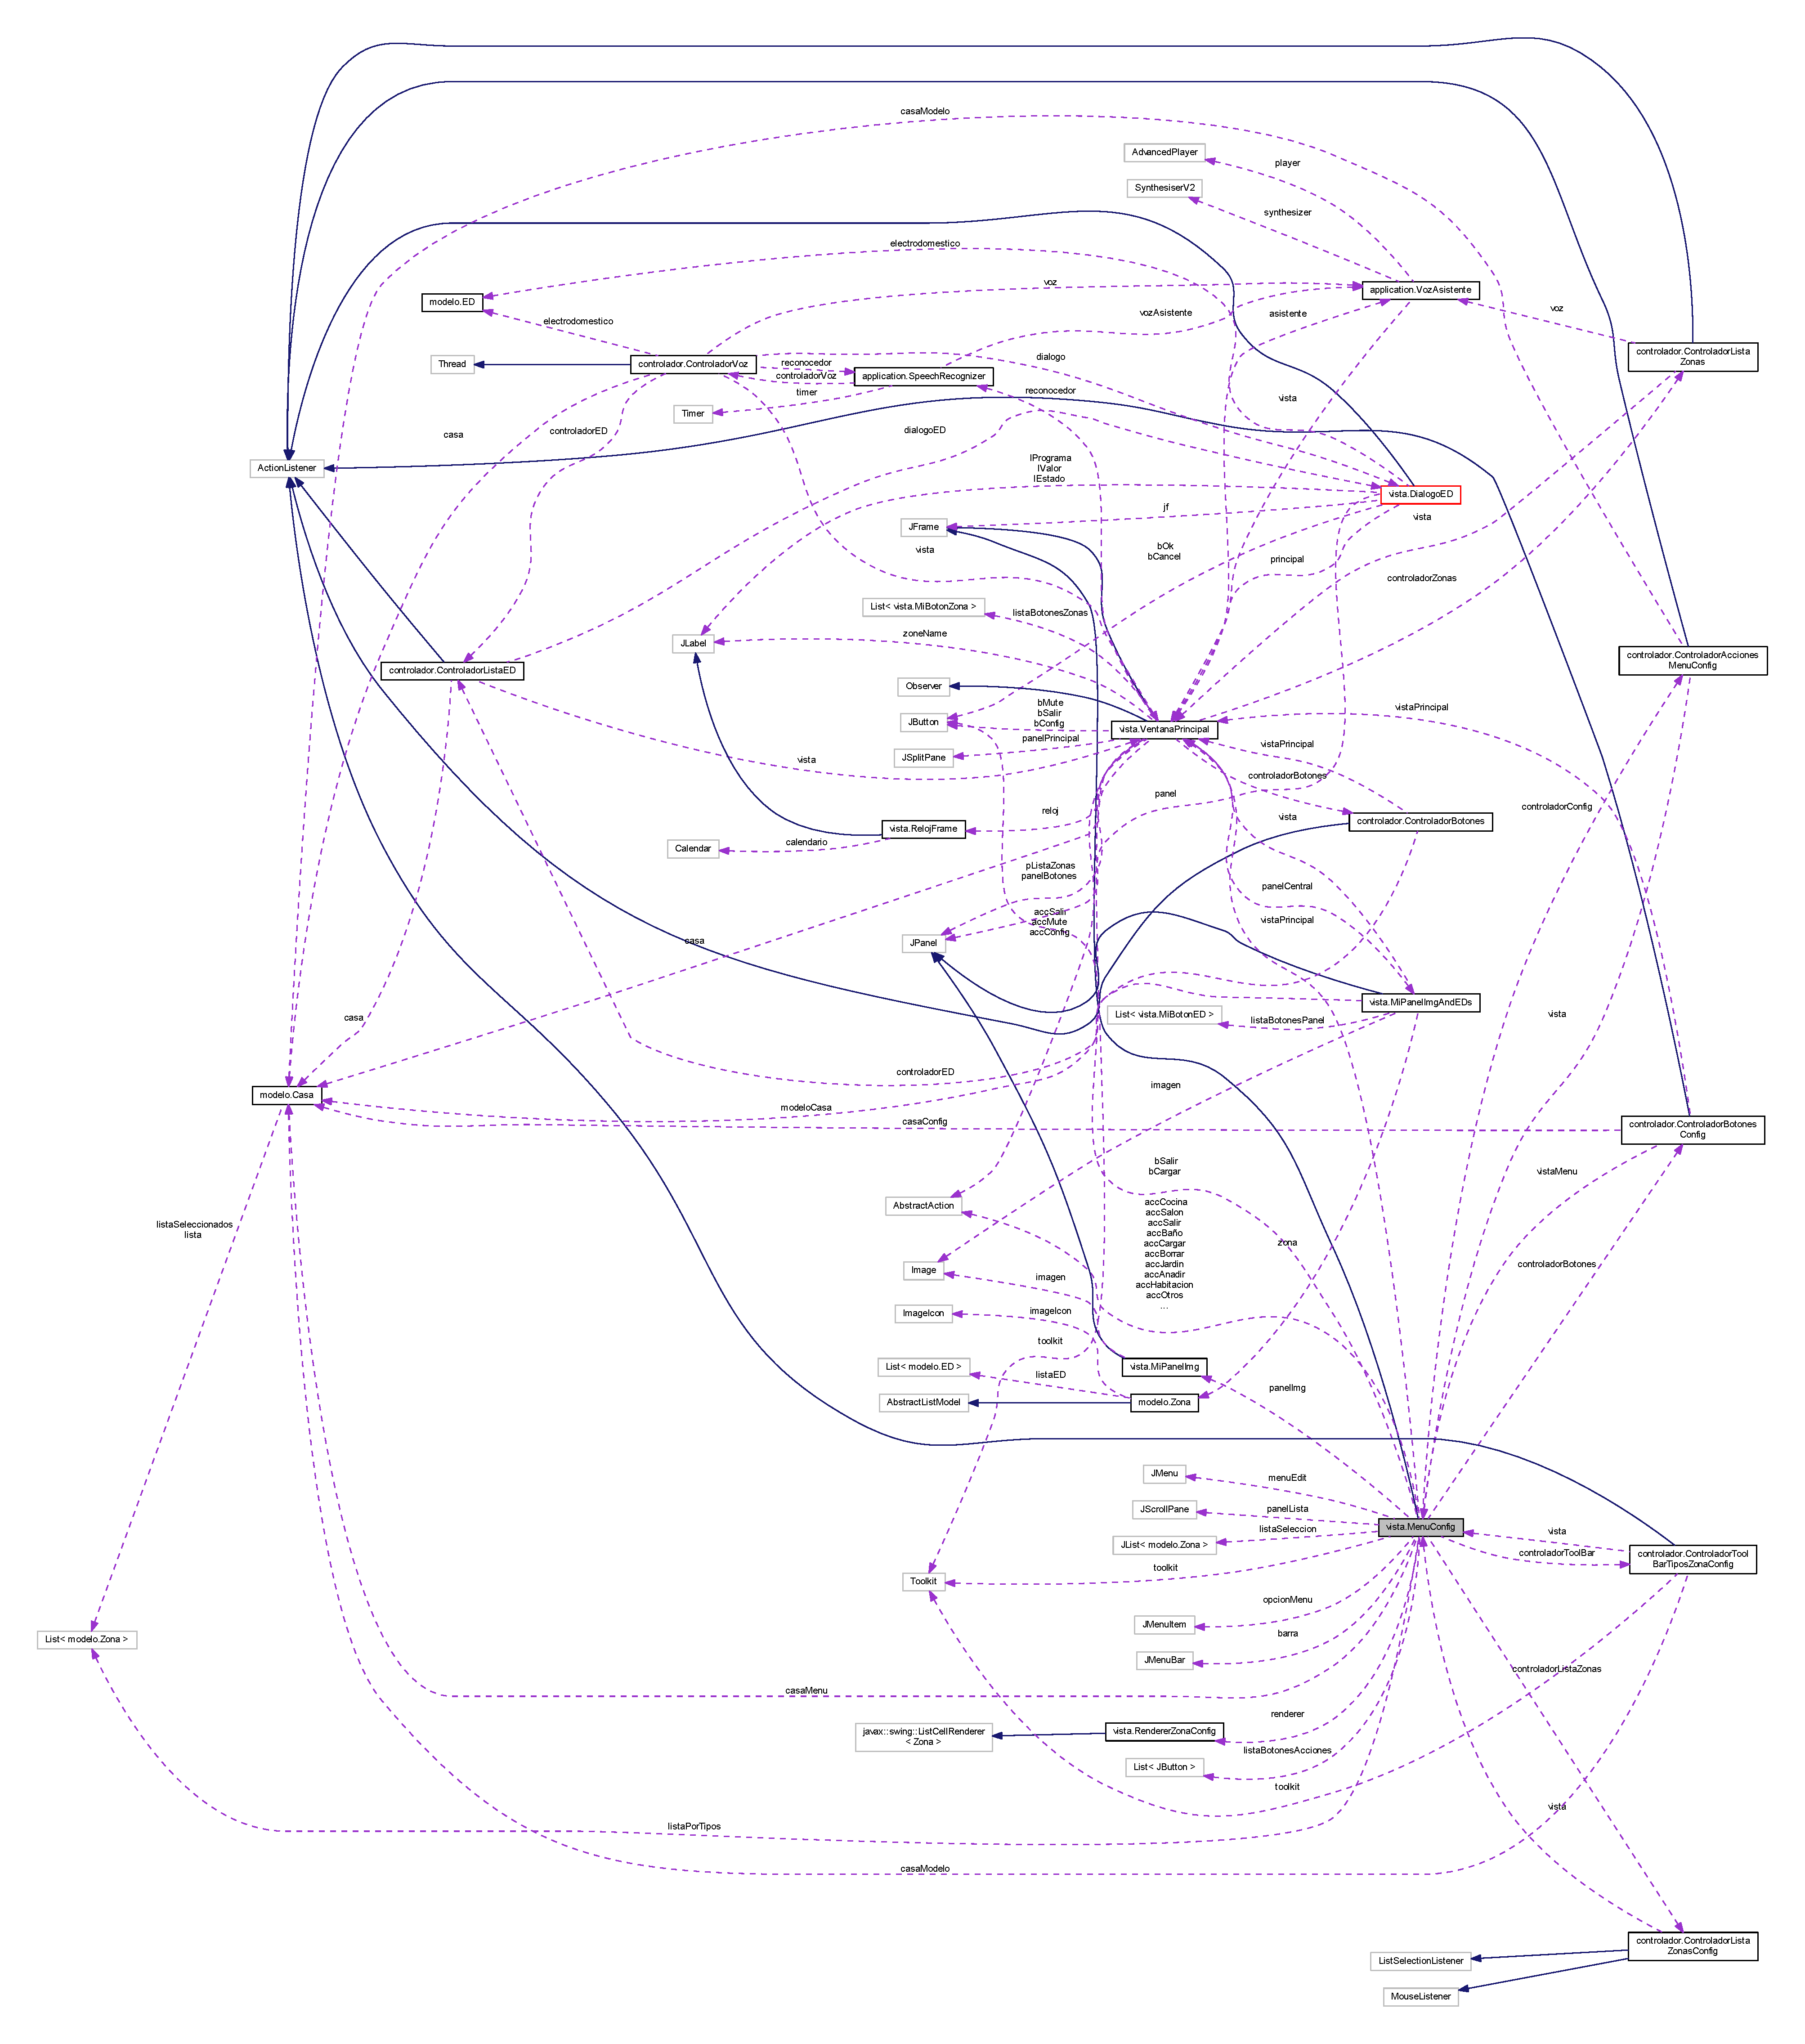
\includegraphics[width=350pt]{classvista_1_1_menu_config__coll__graph}
\end{center}
\end{figure}
\subsection*{Public Member Functions}
\begin{DoxyCompactItemize}
\item 
\mbox{\Hypertarget{classvista_1_1_menu_config_a8816357996dfe08ce3e7e2f1a140676f}\label{classvista_1_1_menu_config_a8816357996dfe08ce3e7e2f1a140676f}} 
{\bfseries Menu\+Config} (\mbox{\hyperlink{classvista_1_1_ventana_principal}{Ventana\+Principal}} vista\+Principal, \mbox{\hyperlink{classmodelo_1_1_casa}{Casa}} casa)
\item 
\mbox{\Hypertarget{classvista_1_1_menu_config_a67a67d59622932be75d810d984872be0}\label{classvista_1_1_menu_config_a67a67d59622932be75d810d984872be0}} 
J\+Button {\bfseries crear\+Boton\+Tool\+Bar} (Abstract\+Action name)
\item 
\mbox{\Hypertarget{classvista_1_1_menu_config_aa025274f7663f42bae01619ad9cb2608}\label{classvista_1_1_menu_config_aa025274f7663f42bae01619ad9cb2608}} 
J\+List$<$ \mbox{\hyperlink{classmodelo_1_1_zona}{Zona}} $>$ {\bfseries get\+Lista\+Seleccion} ()
\item 
\mbox{\Hypertarget{classvista_1_1_menu_config_a750880517f79d71e51129f20b78f149d}\label{classvista_1_1_menu_config_a750880517f79d71e51129f20b78f149d}} 
\mbox{\hyperlink{classvista_1_1_mi_panel_img}{Mi\+Panel\+Img}} {\bfseries get\+Panel\+Img} ()
\item 
\mbox{\Hypertarget{classvista_1_1_menu_config_afe98141e06e8626e4ade8b9d5f04155f}\label{classvista_1_1_menu_config_afe98141e06e8626e4ade8b9d5f04155f}} 
List$<$ J\+Button $>$ {\bfseries get\+Lista\+Botones\+Acciones} ()
\item 
\mbox{\Hypertarget{classvista_1_1_menu_config_a4c3eef77fde182cbf4af1b9d3025424c}\label{classvista_1_1_menu_config_a4c3eef77fde182cbf4af1b9d3025424c}} 
J\+Scroll\+Pane {\bfseries get\+Panel\+Lista} ()
\item 
\mbox{\Hypertarget{classvista_1_1_menu_config_a0ebbf9d5ec630071ee53b2b0cdbc52ef}\label{classvista_1_1_menu_config_a0ebbf9d5ec630071ee53b2b0cdbc52ef}} 
void {\bfseries set\+Actual\+Type} (String actual\+Type)
\item 
\mbox{\Hypertarget{classvista_1_1_menu_config_a88aae2ab7436ffc6a08a5d62c4b8cec3}\label{classvista_1_1_menu_config_a88aae2ab7436ffc6a08a5d62c4b8cec3}} 
String {\bfseries get\+Actual\+Type} ()
\item 
\mbox{\Hypertarget{classvista_1_1_menu_config_acebc3b3ad4cbccf1adf2be86993e7be6}\label{classvista_1_1_menu_config_acebc3b3ad4cbccf1adf2be86993e7be6}} 
\mbox{\hyperlink{classmodelo_1_1_casa}{Casa}} {\bfseries get\+Casa} ()
\item 
\mbox{\Hypertarget{classvista_1_1_menu_config_ac8e0381bd5316a1bca4eeae90a1570a9}\label{classvista_1_1_menu_config_ac8e0381bd5316a1bca4eeae90a1570a9}} 
\mbox{\hyperlink{classmodelo_1_1_zona}{Zona}} {\bfseries get\+Selected\+Zone} ()
\item 
\mbox{\Hypertarget{classvista_1_1_menu_config_af350e1398cbcb22c4c621cc7216bc37e}\label{classvista_1_1_menu_config_af350e1398cbcb22c4c621cc7216bc37e}} 
void {\bfseries update\+List} ()
\end{DoxyCompactItemize}


The documentation for this class was generated from the following file\+:\begin{DoxyCompactItemize}
\item 
C\+:/\+Users/\+Ander/\+Documents/\+Java/\+Dream\+Housev2/src/vista/Menu\+Config.\+java\end{DoxyCompactItemize}

\hypertarget{classvista_1_1_mi_boton_e_d}{}\section{vista.\+Mi\+Boton\+ED Class Reference}
\label{classvista_1_1_mi_boton_e_d}\index{vista.\+Mi\+Boton\+ED@{vista.\+Mi\+Boton\+ED}}


Inheritance diagram for vista.\+Mi\+Boton\+ED\+:
\nopagebreak
\begin{figure}[H]
\begin{center}
\leavevmode
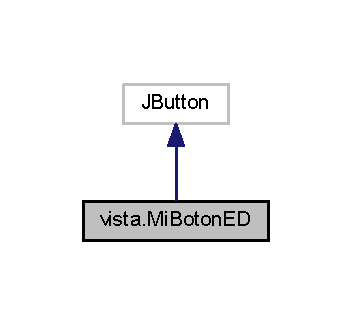
\includegraphics[width=169pt]{classvista_1_1_mi_boton_e_d__inherit__graph}
\end{center}
\end{figure}


Collaboration diagram for vista.\+Mi\+Boton\+ED\+:
\nopagebreak
\begin{figure}[H]
\begin{center}
\leavevmode
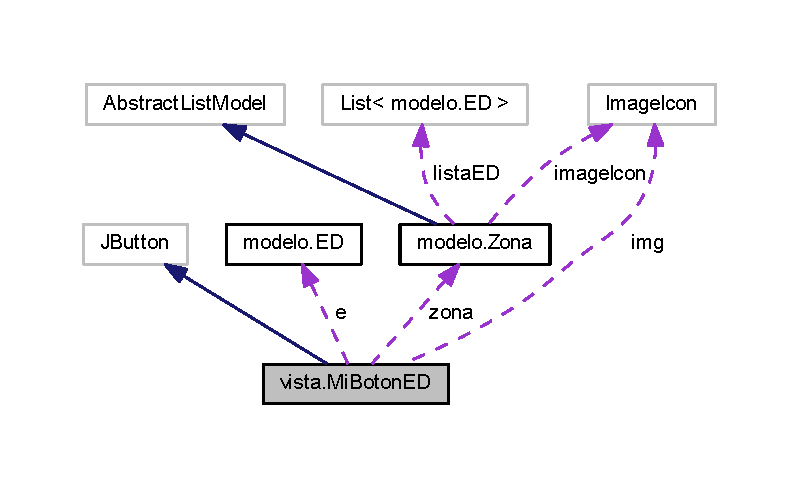
\includegraphics[width=350pt]{classvista_1_1_mi_boton_e_d__coll__graph}
\end{center}
\end{figure}
\subsection*{Public Member Functions}
\begin{DoxyCompactItemize}
\item 
\mbox{\Hypertarget{classvista_1_1_mi_boton_e_d_a6bf8b2b884c0f583021de69e0a7eea73}\label{classvista_1_1_mi_boton_e_d_a6bf8b2b884c0f583021de69e0a7eea73}} 
{\bfseries Mi\+Boton\+ED} (\mbox{\hyperlink{classmodelo_1_1_e_d}{ED}} electrodomestico, \mbox{\hyperlink{classmodelo_1_1_zona}{Zona}} zona)
\item 
\mbox{\Hypertarget{classvista_1_1_mi_boton_e_d_a84868d3ea73732ef8fa4385a73e3b3b9}\label{classvista_1_1_mi_boton_e_d_a84868d3ea73732ef8fa4385a73e3b3b9}} 
void {\bfseries paint\+Border} ()
\end{DoxyCompactItemize}


The documentation for this class was generated from the following file\+:\begin{DoxyCompactItemize}
\item 
C\+:/\+Users/\+Ander/\+Documents/\+Java/\+Dream\+Housev2/src/vista/Mi\+Boton\+E\+D.\+java\end{DoxyCompactItemize}

\hypertarget{classvista_1_1_mi_boton_estado}{}\section{vista.\+Mi\+Boton\+Estado Class Reference}
\label{classvista_1_1_mi_boton_estado}\index{vista.\+Mi\+Boton\+Estado@{vista.\+Mi\+Boton\+Estado}}


Inheritance diagram for vista.\+Mi\+Boton\+Estado\+:
\nopagebreak
\begin{figure}[H]
\begin{center}
\leavevmode
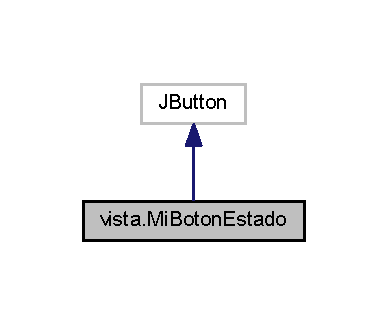
\includegraphics[width=186pt]{classvista_1_1_mi_boton_estado__inherit__graph}
\end{center}
\end{figure}


Collaboration diagram for vista.\+Mi\+Boton\+Estado\+:
\nopagebreak
\begin{figure}[H]
\begin{center}
\leavevmode
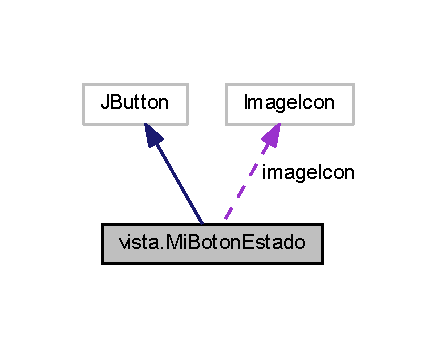
\includegraphics[width=211pt]{classvista_1_1_mi_boton_estado__coll__graph}
\end{center}
\end{figure}
\subsection*{Public Member Functions}
\begin{DoxyCompactItemize}
\item 
\mbox{\Hypertarget{classvista_1_1_mi_boton_estado_ac7a7e4aa70b02f321423183b014e6b20}\label{classvista_1_1_mi_boton_estado_ac7a7e4aa70b02f321423183b014e6b20}} 
{\bfseries Mi\+Boton\+Estado} (Boolean estado)
\item 
\mbox{\Hypertarget{classvista_1_1_mi_boton_estado_a342f778571f033ad6d0ca8c633f1015f}\label{classvista_1_1_mi_boton_estado_a342f778571f033ad6d0ca8c633f1015f}} 
String {\bfseries get\+Nombre} ()
\item 
\mbox{\Hypertarget{classvista_1_1_mi_boton_estado_a6649ee4877d13535560223e9893be0df}\label{classvista_1_1_mi_boton_estado_a6649ee4877d13535560223e9893be0df}} 
void {\bfseries set\+Nombre} (String nombre)
\item 
\mbox{\Hypertarget{classvista_1_1_mi_boton_estado_a3adf7c116ea22a32abb8897401c3272d}\label{classvista_1_1_mi_boton_estado_a3adf7c116ea22a32abb8897401c3272d}} 
void {\bfseries switch\+Status} ()
\item 
\mbox{\Hypertarget{classvista_1_1_mi_boton_estado_a997a9b8cff0e7b872c062cf7844d1c93}\label{classvista_1_1_mi_boton_estado_a997a9b8cff0e7b872c062cf7844d1c93}} 
Boolean {\bfseries get\+Estado} ()
\item 
\mbox{\Hypertarget{classvista_1_1_mi_boton_estado_a767f2c7dac98d8a235c957f1c4e01b8c}\label{classvista_1_1_mi_boton_estado_a767f2c7dac98d8a235c957f1c4e01b8c}} 
void {\bfseries set\+Estado} (Boolean estado)
\item 
\mbox{\Hypertarget{classvista_1_1_mi_boton_estado_ad4d9724658d80cbfc47afd59fe5833ef}\label{classvista_1_1_mi_boton_estado_ad4d9724658d80cbfc47afd59fe5833ef}} 
void {\bfseries set\+Image\+Icon} (Image\+Icon image\+Icon)
\end{DoxyCompactItemize}


The documentation for this class was generated from the following file\+:\begin{DoxyCompactItemize}
\item 
C\+:/\+Users/\+Ander/\+Documents/\+Java/\+Dream\+Housev2/src/vista/Mi\+Boton\+Estado.\+java\end{DoxyCompactItemize}

\hypertarget{classvista_1_1_mi_boton_zona}{}\section{vista.\+Mi\+Boton\+Zona Class Reference}
\label{classvista_1_1_mi_boton_zona}\index{vista.\+Mi\+Boton\+Zona@{vista.\+Mi\+Boton\+Zona}}


Inheritance diagram for vista.\+Mi\+Boton\+Zona\+:
\nopagebreak
\begin{figure}[H]
\begin{center}
\leavevmode
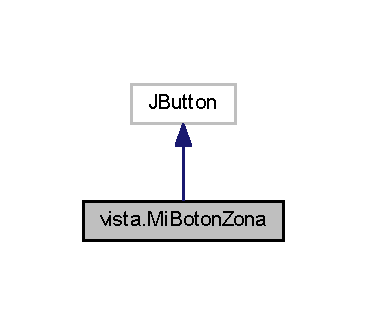
\includegraphics[width=176pt]{classvista_1_1_mi_boton_zona__inherit__graph}
\end{center}
\end{figure}


Collaboration diagram for vista.\+Mi\+Boton\+Zona\+:
\nopagebreak
\begin{figure}[H]
\begin{center}
\leavevmode
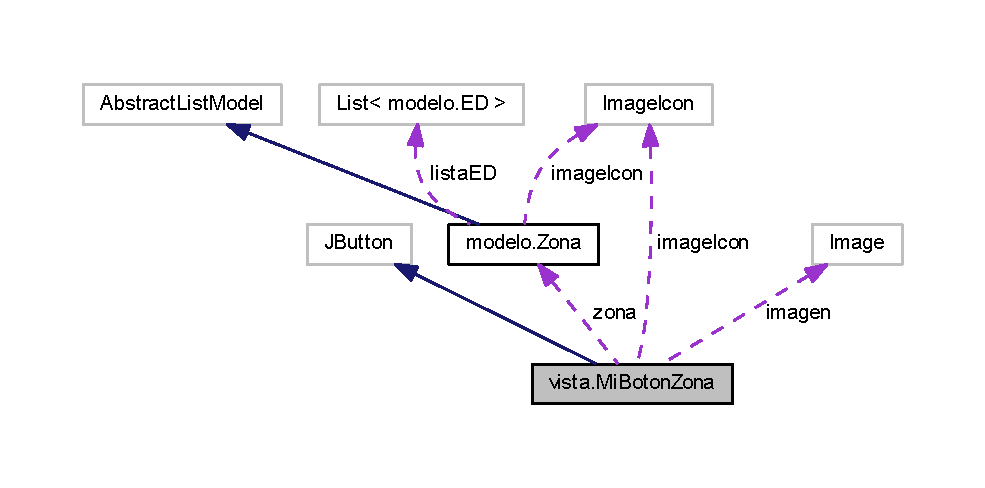
\includegraphics[width=350pt]{classvista_1_1_mi_boton_zona__coll__graph}
\end{center}
\end{figure}
\subsection*{Public Member Functions}
\begin{DoxyCompactItemize}
\item 
\mbox{\Hypertarget{classvista_1_1_mi_boton_zona_a5c7db8e9a25ef3810dfc8fba178d1c78}\label{classvista_1_1_mi_boton_zona_a5c7db8e9a25ef3810dfc8fba178d1c78}} 
{\bfseries Mi\+Boton\+Zona} (\mbox{\hyperlink{classmodelo_1_1_zona}{Zona}} zona, int num\+Zonas)
\item 
\mbox{\Hypertarget{classvista_1_1_mi_boton_zona_ac5964febf18a57ff4b3e563cc30ac2fa}\label{classvista_1_1_mi_boton_zona_ac5964febf18a57ff4b3e563cc30ac2fa}} 
void {\bfseries set\+Zona} (\mbox{\hyperlink{classmodelo_1_1_zona}{Zona}} zona)
\item 
\mbox{\Hypertarget{classvista_1_1_mi_boton_zona_a24c233777bcd781e7d560bea342c4824}\label{classvista_1_1_mi_boton_zona_a24c233777bcd781e7d560bea342c4824}} 
Image {\bfseries get\+Imagen} ()
\item 
\mbox{\Hypertarget{classvista_1_1_mi_boton_zona_a1ee248301e0b3a6c07ba4e0b6e43f8a7}\label{classvista_1_1_mi_boton_zona_a1ee248301e0b3a6c07ba4e0b6e43f8a7}} 
void {\bfseries set\+Imagen} (Image nueva\+Imagen)
\item 
\mbox{\Hypertarget{classvista_1_1_mi_boton_zona_a7e603b1af30532a70204b3aa85ec72ea}\label{classvista_1_1_mi_boton_zona_a7e603b1af30532a70204b3aa85ec72ea}} 
\mbox{\hyperlink{classmodelo_1_1_zona}{Zona}} {\bfseries get\+Zona} ()
\item 
\mbox{\Hypertarget{classvista_1_1_mi_boton_zona_a9fca131b63c836c783e27e0c3f649b97}\label{classvista_1_1_mi_boton_zona_a9fca131b63c836c783e27e0c3f649b97}} 
Image\+Icon {\bfseries get\+Image\+Icon} ()
\item 
\mbox{\Hypertarget{classvista_1_1_mi_boton_zona_a642b9f1a6875fbb25a818c29329ac1c3}\label{classvista_1_1_mi_boton_zona_a642b9f1a6875fbb25a818c29329ac1c3}} 
String {\bfseries get\+Name} ()
\end{DoxyCompactItemize}


The documentation for this class was generated from the following file\+:\begin{DoxyCompactItemize}
\item 
C\+:/\+Users/\+Ander/\+Documents/\+Java/\+Dream\+Housev2/src/vista/Mi\+Boton\+Zona.\+java\end{DoxyCompactItemize}

\hypertarget{classvista_1_1_mi_panel_img}{}\section{vista.\+Mi\+Panel\+Img Class Reference}
\label{classvista_1_1_mi_panel_img}\index{vista.\+Mi\+Panel\+Img@{vista.\+Mi\+Panel\+Img}}


Inheritance diagram for vista.\+Mi\+Panel\+Img\+:
\nopagebreak
\begin{figure}[H]
\begin{center}
\leavevmode
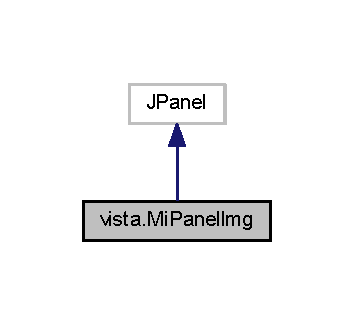
\includegraphics[width=170pt]{classvista_1_1_mi_panel_img__inherit__graph}
\end{center}
\end{figure}


Collaboration diagram for vista.\+Mi\+Panel\+Img\+:
\nopagebreak
\begin{figure}[H]
\begin{center}
\leavevmode
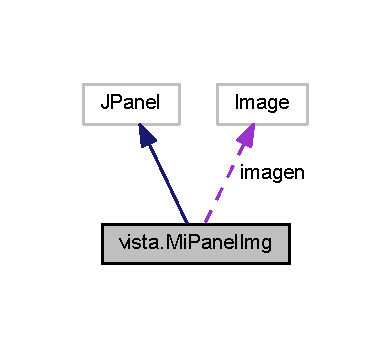
\includegraphics[width=188pt]{classvista_1_1_mi_panel_img__coll__graph}
\end{center}
\end{figure}
\subsection*{Public Member Functions}
\begin{DoxyCompactItemize}
\item 
\mbox{\Hypertarget{classvista_1_1_mi_panel_img_a7350fdda1a38fd8b1a4994cfedcde13c}\label{classvista_1_1_mi_panel_img_a7350fdda1a38fd8b1a4994cfedcde13c}} 
{\bfseries Mi\+Panel\+Img} (Image imagen)
\item 
\mbox{\Hypertarget{classvista_1_1_mi_panel_img_a942afea9ab9fd9a6dbde01493f0e00a1}\label{classvista_1_1_mi_panel_img_a942afea9ab9fd9a6dbde01493f0e00a1}} 
void {\bfseries set\+Imagen} (Image nueva\+Imagen)
\end{DoxyCompactItemize}
\subsection*{Protected Member Functions}
\begin{DoxyCompactItemize}
\item 
\mbox{\Hypertarget{classvista_1_1_mi_panel_img_af77d7ca2dae07436d36a06c31f00d6e1}\label{classvista_1_1_mi_panel_img_af77d7ca2dae07436d36a06c31f00d6e1}} 
void {\bfseries paint\+Component} (Graphics g)
\end{DoxyCompactItemize}


The documentation for this class was generated from the following file\+:\begin{DoxyCompactItemize}
\item 
C\+:/\+Users/\+Ander/\+Documents/\+Java/\+Dream\+Housev2/src/vista/Mi\+Panel\+Img.\+java\end{DoxyCompactItemize}

\hypertarget{classvista_1_1_mi_panel_img_and_e_ds}{}\section{vista.\+Mi\+Panel\+Img\+And\+E\+Ds Class Reference}
\label{classvista_1_1_mi_panel_img_and_e_ds}\index{vista.\+Mi\+Panel\+Img\+And\+E\+Ds@{vista.\+Mi\+Panel\+Img\+And\+E\+Ds}}


Inheritance diagram for vista.\+Mi\+Panel\+Img\+And\+E\+Ds\+:
\nopagebreak
\begin{figure}[H]
\begin{center}
\leavevmode
\includegraphics[width=206pt]{classvista_1_1_mi_panel_img_and_e_ds__inherit__graph}
\end{center}
\end{figure}


Collaboration diagram for vista.\+Mi\+Panel\+Img\+And\+E\+Ds\+:
\nopagebreak
\begin{figure}[H]
\begin{center}
\leavevmode
\includegraphics[width=350pt]{classvista_1_1_mi_panel_img_and_e_ds__coll__graph}
\end{center}
\end{figure}
\subsection*{Public Member Functions}
\begin{DoxyCompactItemize}
\item 
\mbox{\Hypertarget{classvista_1_1_mi_panel_img_and_e_ds_a9a05707bd842a8c78a8b0c188f342ebc}\label{classvista_1_1_mi_panel_img_and_e_ds_a9a05707bd842a8c78a8b0c188f342ebc}} 
{\bfseries Mi\+Panel\+Img\+And\+E\+Ds} (Image imagen, \mbox{\hyperlink{classvista_1_1_ventana_principal}{Ventana\+Principal}} vista, \mbox{\hyperlink{classmodelo_1_1_casa}{Casa}} casa)
\item 
\mbox{\Hypertarget{classvista_1_1_mi_panel_img_and_e_ds_ad6fe7d3e2ceb875550c2933a2fb4a03b}\label{classvista_1_1_mi_panel_img_and_e_ds_ad6fe7d3e2ceb875550c2933a2fb4a03b}} 
Image {\bfseries get\+Imagen} ()
\item 
\mbox{\Hypertarget{classvista_1_1_mi_panel_img_and_e_ds_a25e4fda0b1fd6e037498c3478478018a}\label{classvista_1_1_mi_panel_img_and_e_ds_a25e4fda0b1fd6e037498c3478478018a}} 
void {\bfseries set\+Imagen} (Image nueva\+Imagen)
\item 
\mbox{\Hypertarget{classvista_1_1_mi_panel_img_and_e_ds_a4b474e495661a6c188a2ea5aceabab61}\label{classvista_1_1_mi_panel_img_and_e_ds_a4b474e495661a6c188a2ea5aceabab61}} 
void {\bfseries set\+Zona} (\mbox{\hyperlink{classmodelo_1_1_zona}{Zona}} zona)
\item 
\mbox{\Hypertarget{classvista_1_1_mi_panel_img_and_e_ds_af761a5a5e1f4ba64e828bdfbda12f20d}\label{classvista_1_1_mi_panel_img_and_e_ds_af761a5a5e1f4ba64e828bdfbda12f20d}} 
List$<$ \mbox{\hyperlink{classvista_1_1_mi_boton_e_d}{Mi\+Boton\+ED}} $>$ {\bfseries get\+Lista\+Botones\+Panel} ()
\item 
\mbox{\Hypertarget{classvista_1_1_mi_panel_img_and_e_ds_a6a3da428a1236e42368d53842486ff3f}\label{classvista_1_1_mi_panel_img_and_e_ds_a6a3da428a1236e42368d53842486ff3f}} 
\mbox{\hyperlink{classcontrolador_1_1_controlador_lista_e_d}{Controlador\+Lista\+ED}} {\bfseries get\+Controlador\+ED} ()
\end{DoxyCompactItemize}
\subsection*{Protected Member Functions}
\begin{DoxyCompactItemize}
\item 
\mbox{\Hypertarget{classvista_1_1_mi_panel_img_and_e_ds_abb385fe3b946590d52a1a7373e1fdda5}\label{classvista_1_1_mi_panel_img_and_e_ds_abb385fe3b946590d52a1a7373e1fdda5}} 
void {\bfseries paint\+Component} (Graphics g)
\end{DoxyCompactItemize}


The documentation for this class was generated from the following file\+:\begin{DoxyCompactItemize}
\item 
C\+:/\+Users/\+Ander/\+Documents/\+Java/\+Dream\+Housev2/src/vista/Mi\+Panel\+Img\+And\+E\+Ds.\+java\end{DoxyCompactItemize}

\hypertarget{classvista_1_1_reloj_frame}{}\section{vista.\+Reloj\+Frame Class Reference}
\label{classvista_1_1_reloj_frame}\index{vista.\+Reloj\+Frame@{vista.\+Reloj\+Frame}}


Inheritance diagram for vista.\+Reloj\+Frame\+:
\nopagebreak
\begin{figure}[H]
\begin{center}
\leavevmode
\includegraphics[width=169pt]{classvista_1_1_reloj_frame__inherit__graph}
\end{center}
\end{figure}


Collaboration diagram for vista.\+Reloj\+Frame\+:
\nopagebreak
\begin{figure}[H]
\begin{center}
\leavevmode
\includegraphics[width=204pt]{classvista_1_1_reloj_frame__coll__graph}
\end{center}
\end{figure}
\subsection*{Public Member Functions}
\begin{DoxyCompactItemize}
\item 
\mbox{\Hypertarget{classvista_1_1_reloj_frame_a265ed4e08edcc3d106a9e64448e65abe}\label{classvista_1_1_reloj_frame_a265ed4e08edcc3d106a9e64448e65abe}} 
J\+Label {\bfseries get\+Label} ()
\end{DoxyCompactItemize}


The documentation for this class was generated from the following file\+:\begin{DoxyCompactItemize}
\item 
C\+:/\+Users/\+Ander/\+Documents/\+Java/\+Dream\+Housev2/src/vista/Reloj\+Frame.\+java\end{DoxyCompactItemize}

\hypertarget{classvista_1_1_renderer_e_d_config}{}\section{vista.\+Renderer\+E\+D\+Config Class Reference}
\label{classvista_1_1_renderer_e_d_config}\index{vista.\+Renderer\+E\+D\+Config@{vista.\+Renderer\+E\+D\+Config}}


Inheritance diagram for vista.\+Renderer\+E\+D\+Config\+:
\nopagebreak
\begin{figure}[H]
\begin{center}
\leavevmode
\includegraphics[width=226pt]{classvista_1_1_renderer_e_d_config__inherit__graph}
\end{center}
\end{figure}


Collaboration diagram for vista.\+Renderer\+E\+D\+Config\+:
\nopagebreak
\begin{figure}[H]
\begin{center}
\leavevmode
\includegraphics[width=226pt]{classvista_1_1_renderer_e_d_config__coll__graph}
\end{center}
\end{figure}
\subsection*{Public Member Functions}
\begin{DoxyCompactItemize}
\item 
\mbox{\Hypertarget{classvista_1_1_renderer_e_d_config_ab2e3d5e37cd5be21f3e147b362970483}\label{classvista_1_1_renderer_e_d_config_ab2e3d5e37cd5be21f3e147b362970483}} 
Component {\bfseries get\+List\+Cell\+Renderer\+Component} (J\+List$<$? extends \mbox{\hyperlink{classmodelo_1_1_e_d}{ED}} $>$ list, \mbox{\hyperlink{classmodelo_1_1_e_d}{ED}} value, int index, boolean is\+Selected, boolean cell\+Has\+Focus)
\end{DoxyCompactItemize}


The documentation for this class was generated from the following file\+:\begin{DoxyCompactItemize}
\item 
C\+:/\+Users/\+Ander/\+Documents/\+Java/\+Dream\+Housev2/src/vista/Renderer\+E\+D\+Config.\+java\end{DoxyCompactItemize}

\hypertarget{classvista_1_1_renderer_zona_config}{}\section{vista.\+Renderer\+Zona\+Config Class Reference}
\label{classvista_1_1_renderer_zona_config}\index{vista.\+Renderer\+Zona\+Config@{vista.\+Renderer\+Zona\+Config}}


Inheritance diagram for vista.\+Renderer\+Zona\+Config\+:
\nopagebreak
\begin{figure}[H]
\begin{center}
\leavevmode
\includegraphics[width=226pt]{classvista_1_1_renderer_zona_config__inherit__graph}
\end{center}
\end{figure}


Collaboration diagram for vista.\+Renderer\+Zona\+Config\+:
\nopagebreak
\begin{figure}[H]
\begin{center}
\leavevmode
\includegraphics[width=226pt]{classvista_1_1_renderer_zona_config__coll__graph}
\end{center}
\end{figure}
\subsection*{Public Member Functions}
\begin{DoxyCompactItemize}
\item 
\mbox{\Hypertarget{classvista_1_1_renderer_zona_config_a79630527664cb2745d0f55dcf719137a}\label{classvista_1_1_renderer_zona_config_a79630527664cb2745d0f55dcf719137a}} 
Component {\bfseries get\+List\+Cell\+Renderer\+Component} (J\+List$<$? extends \mbox{\hyperlink{classmodelo_1_1_zona}{Zona}} $>$ list, \mbox{\hyperlink{classmodelo_1_1_zona}{Zona}} value, int index, boolean is\+Selected, boolean cell\+Has\+Focus)
\end{DoxyCompactItemize}


The documentation for this class was generated from the following file\+:\begin{DoxyCompactItemize}
\item 
C\+:/\+Users/\+Ander/\+Documents/\+Java/\+Dream\+Housev2/src/vista/Renderer\+Zona\+Config.\+java\end{DoxyCompactItemize}

\hypertarget{classvista_1_1_single_root_file_system_view}{}\section{vista.\+Single\+Root\+File\+System\+View Class Reference}
\label{classvista_1_1_single_root_file_system_view}\index{vista.\+Single\+Root\+File\+System\+View@{vista.\+Single\+Root\+File\+System\+View}}


Inheritance diagram for vista.\+Single\+Root\+File\+System\+View\+:
\nopagebreak
\begin{figure}[H]
\begin{center}
\leavevmode
\includegraphics[width=237pt]{classvista_1_1_single_root_file_system_view__inherit__graph}
\end{center}
\end{figure}


Collaboration diagram for vista.\+Single\+Root\+File\+System\+View\+:
\nopagebreak
\begin{figure}[H]
\begin{center}
\leavevmode
\includegraphics[width=241pt]{classvista_1_1_single_root_file_system_view__coll__graph}
\end{center}
\end{figure}
\subsection*{Public Member Functions}
\begin{DoxyCompactItemize}
\item 
\mbox{\Hypertarget{classvista_1_1_single_root_file_system_view_a12c6cd626588f78090c0449a111b38ee}\label{classvista_1_1_single_root_file_system_view_a12c6cd626588f78090c0449a111b38ee}} 
{\bfseries Single\+Root\+File\+System\+View} (File path)
\item 
\mbox{\Hypertarget{classvista_1_1_single_root_file_system_view_abbc2d9a43fd3e8a73900433739f716f9}\label{classvista_1_1_single_root_file_system_view_abbc2d9a43fd3e8a73900433739f716f9}} 
File {\bfseries create\+New\+Folder} (File containing\+Dir)
\item 
\mbox{\Hypertarget{classvista_1_1_single_root_file_system_view_a4160416c2105f1368d3de89ea1bd9f30}\label{classvista_1_1_single_root_file_system_view_a4160416c2105f1368d3de89ea1bd9f30}} 
File {\bfseries get\+Default\+Directory} ()
\item 
\mbox{\Hypertarget{classvista_1_1_single_root_file_system_view_a568ece1a85f1d3e213cbd8a7819aa110}\label{classvista_1_1_single_root_file_system_view_a568ece1a85f1d3e213cbd8a7819aa110}} 
File {\bfseries get\+Home\+Directory} ()
\item 
\mbox{\Hypertarget{classvista_1_1_single_root_file_system_view_a618f89445cbaed2879f3a26a761d8c94}\label{classvista_1_1_single_root_file_system_view_a618f89445cbaed2879f3a26a761d8c94}} 
File \mbox{[}$\,$\mbox{]} {\bfseries get\+Roots} ()
\end{DoxyCompactItemize}


\subsection{Detailed Description}
A File\+System\+View class that limits the file selections to a single root.

When used with the J\+File\+Chooser component the user will only be able to traverse the directories contained within the specified root fill.

The \char`\"{}\+Look In\char`\"{} combo box will only display the specified root.

The \char`\"{}\+Up One Level\char`\"{} button will be disable when at the root. 

The documentation for this class was generated from the following file\+:\begin{DoxyCompactItemize}
\item 
C\+:/\+Users/\+Ander/\+Documents/\+Java/\+Dream\+Housev2/src/vista/Single\+Root\+File\+System\+View.\+java\end{DoxyCompactItemize}

\hypertarget{classapplication_1_1_speech_recognizer}{}\section{application.\+Speech\+Recognizer Class Reference}
\label{classapplication_1_1_speech_recognizer}\index{application.\+Speech\+Recognizer@{application.\+Speech\+Recognizer}}


Collaboration diagram for application.\+Speech\+Recognizer\+:
\nopagebreak
\begin{figure}[H]
\begin{center}
\leavevmode
\includegraphics[width=350pt]{classapplication_1_1_speech_recognizer__coll__graph}
\end{center}
\end{figure}
\subsection*{Classes}
\begin{DoxyCompactItemize}
\item 
class {\bfseries Task}
\end{DoxyCompactItemize}
\subsection*{Public Member Functions}
\begin{DoxyCompactItemize}
\item 
\mbox{\Hypertarget{classapplication_1_1_speech_recognizer_acf64bba8786b912f367e230d195104b2}\label{classapplication_1_1_speech_recognizer_acf64bba8786b912f367e230d195104b2}} 
{\bfseries Speech\+Recognizer} (\mbox{\hyperlink{classvista_1_1_ventana_principal}{Ventana\+Principal}} vista, \mbox{\hyperlink{classmodelo_1_1_casa}{Casa}} casa)
\item 
synchronized void \mbox{\hyperlink{classapplication_1_1_speech_recognizer_a3c3ad8b38751bf186e470dc9e29bec57}{start\+Speech\+Recognition}} (\mbox{\hyperlink{classvista_1_1_ventana_principal}{Ventana\+Principal}} vista)
\item 
synchronized void \mbox{\hyperlink{classapplication_1_1_speech_recognizer_a6c9ee420dd7fcf9b6aeda63361b0c819}{stop\+Ignore\+Speech\+Recognition\+Results}} ()
\item 
synchronized void \mbox{\hyperlink{classapplication_1_1_speech_recognizer_ad3dee52e0a9cd3dbcd9efa1fa6d38033}{ignore\+Speech\+Recognition\+Results}} ()
\item 
void \mbox{\hyperlink{classapplication_1_1_speech_recognizer_a494e51cb32e7ebc01e58ebc43444c387}{start\+Resources\+Thread}} ()
\item 
void \mbox{\hyperlink{classapplication_1_1_speech_recognizer_a52344e31f4d4cec33c0713387a10c235}{Temporizador}} (int segundos)
\item 
\mbox{\Hypertarget{classapplication_1_1_speech_recognizer_a36f81c4e2247525167e24f41a6de25f6}\label{classapplication_1_1_speech_recognizer_a36f81c4e2247525167e24f41a6de25f6}} 
String {\bfseries get\+Palabra} ()
\item 
\mbox{\Hypertarget{classapplication_1_1_speech_recognizer_af426938b9762c29f5a5bfbb3391fe63d}\label{classapplication_1_1_speech_recognizer_af426938b9762c29f5a5bfbb3391fe63d}} 
String {\bfseries get\+Speech} ()
\item 
\mbox{\Hypertarget{classapplication_1_1_speech_recognizer_aa6e25a4037ce514d7d4a6835afbf0db8}\label{classapplication_1_1_speech_recognizer_aa6e25a4037ce514d7d4a6835afbf0db8}} 
boolean {\bfseries get\+Ignore\+Speech\+Recognition\+Results} ()
\item 
\mbox{\Hypertarget{classapplication_1_1_speech_recognizer_a0fc8931dac55b932ee36e4d537a76063}\label{classapplication_1_1_speech_recognizer_a0fc8931dac55b932ee36e4d537a76063}} 
boolean {\bfseries get\+Speech\+Recognizer\+Thread\+Running} ()
\end{DoxyCompactItemize}


\subsection{Member Function Documentation}
\mbox{\Hypertarget{classapplication_1_1_speech_recognizer_ad3dee52e0a9cd3dbcd9efa1fa6d38033}\label{classapplication_1_1_speech_recognizer_ad3dee52e0a9cd3dbcd9efa1fa6d38033}} 
\index{application\+::\+Speech\+Recognizer@{application\+::\+Speech\+Recognizer}!ignore\+Speech\+Recognition\+Results@{ignore\+Speech\+Recognition\+Results}}
\index{ignore\+Speech\+Recognition\+Results@{ignore\+Speech\+Recognition\+Results}!application\+::\+Speech\+Recognizer@{application\+::\+Speech\+Recognizer}}
\subsubsection{\texorpdfstring{ignore\+Speech\+Recognition\+Results()}{ignoreSpeechRecognitionResults()}}
{\footnotesize\ttfamily synchronized void application.\+Speech\+Recognizer.\+ignore\+Speech\+Recognition\+Results (\begin{DoxyParamCaption}{ }\end{DoxyParamCaption})}

Ignores the results of Speech\+Recognition \mbox{\Hypertarget{classapplication_1_1_speech_recognizer_a494e51cb32e7ebc01e58ebc43444c387}\label{classapplication_1_1_speech_recognizer_a494e51cb32e7ebc01e58ebc43444c387}} 
\index{application\+::\+Speech\+Recognizer@{application\+::\+Speech\+Recognizer}!start\+Resources\+Thread@{start\+Resources\+Thread}}
\index{start\+Resources\+Thread@{start\+Resources\+Thread}!application\+::\+Speech\+Recognizer@{application\+::\+Speech\+Recognizer}}
\subsubsection{\texorpdfstring{start\+Resources\+Thread()}{startResourcesThread()}}
{\footnotesize\ttfamily void application.\+Speech\+Recognizer.\+start\+Resources\+Thread (\begin{DoxyParamCaption}{ }\end{DoxyParamCaption})}

Starting a Thread that checks if the resources needed to the Speech\+Recognition library are available \mbox{\Hypertarget{classapplication_1_1_speech_recognizer_a3c3ad8b38751bf186e470dc9e29bec57}\label{classapplication_1_1_speech_recognizer_a3c3ad8b38751bf186e470dc9e29bec57}} 
\index{application\+::\+Speech\+Recognizer@{application\+::\+Speech\+Recognizer}!start\+Speech\+Recognition@{start\+Speech\+Recognition}}
\index{start\+Speech\+Recognition@{start\+Speech\+Recognition}!application\+::\+Speech\+Recognizer@{application\+::\+Speech\+Recognizer}}
\subsubsection{\texorpdfstring{start\+Speech\+Recognition()}{startSpeechRecognition()}}
{\footnotesize\ttfamily synchronized void application.\+Speech\+Recognizer.\+start\+Speech\+Recognition (\begin{DoxyParamCaption}\item[{\mbox{\hyperlink{classvista_1_1_ventana_principal}{Ventana\+Principal}}}]{vista }\end{DoxyParamCaption})}

Starts the Speech Recognition Thread \mbox{\Hypertarget{classapplication_1_1_speech_recognizer_a6c9ee420dd7fcf9b6aeda63361b0c819}\label{classapplication_1_1_speech_recognizer_a6c9ee420dd7fcf9b6aeda63361b0c819}} 
\index{application\+::\+Speech\+Recognizer@{application\+::\+Speech\+Recognizer}!stop\+Ignore\+Speech\+Recognition\+Results@{stop\+Ignore\+Speech\+Recognition\+Results}}
\index{stop\+Ignore\+Speech\+Recognition\+Results@{stop\+Ignore\+Speech\+Recognition\+Results}!application\+::\+Speech\+Recognizer@{application\+::\+Speech\+Recognizer}}
\subsubsection{\texorpdfstring{stop\+Ignore\+Speech\+Recognition\+Results()}{stopIgnoreSpeechRecognitionResults()}}
{\footnotesize\ttfamily synchronized void application.\+Speech\+Recognizer.\+stop\+Ignore\+Speech\+Recognition\+Results (\begin{DoxyParamCaption}{ }\end{DoxyParamCaption})}

Stops ignoring the results of Speech\+Recognition \mbox{\Hypertarget{classapplication_1_1_speech_recognizer_a52344e31f4d4cec33c0713387a10c235}\label{classapplication_1_1_speech_recognizer_a52344e31f4d4cec33c0713387a10c235}} 
\index{application\+::\+Speech\+Recognizer@{application\+::\+Speech\+Recognizer}!Temporizador@{Temporizador}}
\index{Temporizador@{Temporizador}!application\+::\+Speech\+Recognizer@{application\+::\+Speech\+Recognizer}}
\subsubsection{\texorpdfstring{Temporizador()}{Temporizador()}}
{\footnotesize\ttfamily void application.\+Speech\+Recognizer.\+Temporizador (\begin{DoxyParamCaption}\item[{int}]{segundos }\end{DoxyParamCaption})}

Timer 

The documentation for this class was generated from the following file\+:\begin{DoxyCompactItemize}
\item 
C\+:/\+Users/\+Ander/\+Documents/\+Java/\+Dream\+Housev2/src/application/Speech\+Recognizer.\+java\end{DoxyCompactItemize}

\hypertarget{classvista_1_1_ventana_principal}{}\section{vista.\+Ventana\+Principal Class Reference}
\label{classvista_1_1_ventana_principal}\index{vista.\+Ventana\+Principal@{vista.\+Ventana\+Principal}}


Inheritance diagram for vista.\+Ventana\+Principal\+:
\nopagebreak
\begin{figure}[H]
\begin{center}
\leavevmode
\includegraphics[width=202pt]{classvista_1_1_ventana_principal__inherit__graph}
\end{center}
\end{figure}


Collaboration diagram for vista.\+Ventana\+Principal\+:
\nopagebreak
\begin{figure}[H]
\begin{center}
\leavevmode
\includegraphics[width=350pt]{classvista_1_1_ventana_principal__coll__graph}
\end{center}
\end{figure}
\subsection*{Public Member Functions}
\begin{DoxyCompactItemize}
\item 
\mbox{\Hypertarget{classvista_1_1_ventana_principal_aac56c6c6f900b7a17c1797f343f68164}\label{classvista_1_1_ventana_principal_aac56c6c6f900b7a17c1797f343f68164}} 
void {\bfseries mi\+Repintar} ()
\item 
\mbox{\Hypertarget{classvista_1_1_ventana_principal_a3d43755ba8664a494b1f79b97b82184a}\label{classvista_1_1_ventana_principal_a3d43755ba8664a494b1f79b97b82184a}} 
void {\bfseries update} (Observable arg0, Object arg1)
\item 
\mbox{\Hypertarget{classvista_1_1_ventana_principal_a1b0d8e63220452c9089ff1f2ba863387}\label{classvista_1_1_ventana_principal_a1b0d8e63220452c9089ff1f2ba863387}} 
List$<$ \mbox{\hyperlink{classvista_1_1_mi_boton_zona}{Mi\+Boton\+Zona}} $>$ {\bfseries get\+Lista\+Botones\+Zonas} ()
\item 
\mbox{\Hypertarget{classvista_1_1_ventana_principal_a279cf62616a4bff041a1d0404bbcc89d}\label{classvista_1_1_ventana_principal_a279cf62616a4bff041a1d0404bbcc89d}} 
\mbox{\hyperlink{classvista_1_1_mi_boton_zona}{Mi\+Boton\+Zona}} {\bfseries get\+Boton\+Lista} (String name)
\item 
\mbox{\Hypertarget{classvista_1_1_ventana_principal_ad8b984ff16c9841f85d1d7b40b8a75e6}\label{classvista_1_1_ventana_principal_ad8b984ff16c9841f85d1d7b40b8a75e6}} 
List$<$ \mbox{\hyperlink{classvista_1_1_mi_boton_e_d}{Mi\+Boton\+ED}} $>$ {\bfseries get\+Lista\+Botones\+E\+Ds} ()
\item 
\mbox{\Hypertarget{classvista_1_1_ventana_principal_a58cc9285cb9179a66284f52a2e7d0dd9}\label{classvista_1_1_ventana_principal_a58cc9285cb9179a66284f52a2e7d0dd9}} 
\mbox{\hyperlink{classmodelo_1_1_zona}{Zona}} {\bfseries get\+Zona\+Actual} ()
\item 
\mbox{\Hypertarget{classvista_1_1_ventana_principal_a1534a5187e8ce83f76c44abc02cb2236}\label{classvista_1_1_ventana_principal_a1534a5187e8ce83f76c44abc02cb2236}} 
J\+Label {\bfseries get\+Zone\+Name} ()
\item 
\mbox{\Hypertarget{classvista_1_1_ventana_principal_a7303665d4193ebf7c4693846114fb96d}\label{classvista_1_1_ventana_principal_a7303665d4193ebf7c4693846114fb96d}} 
int {\bfseries get\+Num\+Zonas} ()
\item 
\mbox{\Hypertarget{classvista_1_1_ventana_principal_a740a2cfb769129790ed6026fba51988b}\label{classvista_1_1_ventana_principal_a740a2cfb769129790ed6026fba51988b}} 
int {\bfseries get\+Flag} ()
\item 
\mbox{\Hypertarget{classvista_1_1_ventana_principal_a355d4483232fb23eb4b2e1c27c7086a9}\label{classvista_1_1_ventana_principal_a355d4483232fb23eb4b2e1c27c7086a9}} 
void {\bfseries set\+Flag} (int flag)
\item 
\mbox{\Hypertarget{classvista_1_1_ventana_principal_a95bbd92b1f1d270c58f62c6004efa0f3}\label{classvista_1_1_ventana_principal_a95bbd92b1f1d270c58f62c6004efa0f3}} 
J\+Panel {\bfseries getp\+Lista\+Zonas} ()
\item 
\mbox{\Hypertarget{classvista_1_1_ventana_principal_a34c5b655d700623d5a936f252211f80e}\label{classvista_1_1_ventana_principal_a34c5b655d700623d5a936f252211f80e}} 
\mbox{\hyperlink{classvista_1_1_mi_panel_img_and_e_ds}{Mi\+Panel\+Img\+And\+E\+Ds}} {\bfseries get\+Panel\+Central} ()
\item 
\mbox{\Hypertarget{classvista_1_1_ventana_principal_aee94264e918d71a71fb001bb26aaa3dc}\label{classvista_1_1_ventana_principal_aee94264e918d71a71fb001bb26aaa3dc}} 
J\+Button {\bfseries getb\+Mute} ()
\item 
\mbox{\Hypertarget{classvista_1_1_ventana_principal_a908035b3b52dfaf391f1f6453ecb9565}\label{classvista_1_1_ventana_principal_a908035b3b52dfaf391f1f6453ecb9565}} 
Boolean {\bfseries get\+Mute} ()
\item 
\mbox{\Hypertarget{classvista_1_1_ventana_principal_a22637ae07a73f26d3f975a9d46d1acea}\label{classvista_1_1_ventana_principal_a22637ae07a73f26d3f975a9d46d1acea}} 
void {\bfseries set\+Mute} (Boolean mute)
\end{DoxyCompactItemize}
\subsection*{Static Public Member Functions}
\begin{DoxyCompactItemize}
\item 
\mbox{\Hypertarget{classvista_1_1_ventana_principal_ae492857ab0e8a1bdc5161177cb1d127e}\label{classvista_1_1_ventana_principal_ae492857ab0e8a1bdc5161177cb1d127e}} 
static void {\bfseries main} (String\mbox{[}$\,$\mbox{]} args)
\end{DoxyCompactItemize}


The documentation for this class was generated from the following file\+:\begin{DoxyCompactItemize}
\item 
C\+:/\+Users/\+Ander/\+Documents/\+Java/\+Dream\+Housev2/src/vista/Ventana\+Principal.\+java\end{DoxyCompactItemize}

\hypertarget{classapplication_1_1_voz_asistente}{}\section{application.\+Voz\+Asistente Class Reference}
\label{classapplication_1_1_voz_asistente}\index{application.\+Voz\+Asistente@{application.\+Voz\+Asistente}}


Collaboration diagram for application.\+Voz\+Asistente\+:
\nopagebreak
\begin{figure}[H]
\begin{center}
\leavevmode
\includegraphics[width=350pt]{classapplication_1_1_voz_asistente__coll__graph}
\end{center}
\end{figure}
\subsection*{Public Member Functions}
\begin{DoxyCompactItemize}
\item 
\mbox{\hyperlink{classapplication_1_1_voz_asistente_abbcb08ba9e4c065c9c40c2d0e554808b}{Voz\+Asistente}} (\mbox{\hyperlink{classvista_1_1_ventana_principal}{Ventana\+Principal}} vista)
\item 
\mbox{\Hypertarget{classapplication_1_1_voz_asistente_adc472387531a7d0bdbb256278ab58828}\label{classapplication_1_1_voz_asistente_adc472387531a7d0bdbb256278ab58828}} 
void {\bfseries speak} (String text)
\end{DoxyCompactItemize}


\subsection{Detailed Description}
This is where all begins .

\begin{DoxyAuthor}{Author}
G\+O\+X\+R3\+P\+L\+US 
\end{DoxyAuthor}


\subsection{Constructor \& Destructor Documentation}
\mbox{\Hypertarget{classapplication_1_1_voz_asistente_abbcb08ba9e4c065c9c40c2d0e554808b}\label{classapplication_1_1_voz_asistente_abbcb08ba9e4c065c9c40c2d0e554808b}} 
\index{application\+::\+Voz\+Asistente@{application\+::\+Voz\+Asistente}!Voz\+Asistente@{Voz\+Asistente}}
\index{Voz\+Asistente@{Voz\+Asistente}!application\+::\+Voz\+Asistente@{application\+::\+Voz\+Asistente}}
\subsubsection{\texorpdfstring{Voz\+Asistente()}{VozAsistente()}}
{\footnotesize\ttfamily application.\+Voz\+Asistente.\+Voz\+Asistente (\begin{DoxyParamCaption}\item[{\mbox{\hyperlink{classvista_1_1_ventana_principal}{Ventana\+Principal}}}]{vista }\end{DoxyParamCaption})}

Constructor 

The documentation for this class was generated from the following file\+:\begin{DoxyCompactItemize}
\item 
C\+:/\+Users/\+Ander/\+Documents/\+Java/\+Dream\+Housev2/src/application/Voz\+Asistente.\+java\end{DoxyCompactItemize}

\hypertarget{classmodelo_1_1_zona}{}\section{modelo.\+Zona Class Reference}
\label{classmodelo_1_1_zona}\index{modelo.\+Zona@{modelo.\+Zona}}


Inheritance diagram for modelo.\+Zona\+:
\nopagebreak
\begin{figure}[H]
\begin{center}
\leavevmode
\includegraphics[width=175pt]{classmodelo_1_1_zona__inherit__graph}
\end{center}
\end{figure}


Collaboration diagram for modelo.\+Zona\+:
\nopagebreak
\begin{figure}[H]
\begin{center}
\leavevmode
\includegraphics[width=350pt]{classmodelo_1_1_zona__coll__graph}
\end{center}
\end{figure}
\subsection*{Public Member Functions}
\begin{DoxyCompactItemize}
\item 
\mbox{\Hypertarget{classmodelo_1_1_zona_a1be4bcab3ca76125a2ab065bb4d79114}\label{classmodelo_1_1_zona_a1be4bcab3ca76125a2ab065bb4d79114}} 
{\bfseries Zona} (String name, String imagen)
\item 
\mbox{\Hypertarget{classmodelo_1_1_zona_a0866956d21be4423b0a4b6292b349f6e}\label{classmodelo_1_1_zona_a0866956d21be4423b0a4b6292b349f6e}} 
{\bfseries Zona} (String linea)
\item 
\mbox{\Hypertarget{classmodelo_1_1_zona_a1697e1ce1aaa4574a30e6519546bf214}\label{classmodelo_1_1_zona_a1697e1ce1aaa4574a30e6519546bf214}} 
String {\bfseries to\+String\+File} ()
\item 
\mbox{\Hypertarget{classmodelo_1_1_zona_a5e285ed339ef7daee4021c7cab1bcac4}\label{classmodelo_1_1_zona_a5e285ed339ef7daee4021c7cab1bcac4}} 
String {\bfseries to\+String} ()
\item 
\mbox{\Hypertarget{classmodelo_1_1_zona_aa7241417dbf1153844826e19e9be1112}\label{classmodelo_1_1_zona_aa7241417dbf1153844826e19e9be1112}} 
int {\bfseries get\+Next\+Value} (String tipo)
\item 
\mbox{\Hypertarget{classmodelo_1_1_zona_ab133c3ea1a52d41ab1cd9aa2401f68f6}\label{classmodelo_1_1_zona_ab133c3ea1a52d41ab1cd9aa2401f68f6}} 
List$<$ \mbox{\hyperlink{classmodelo_1_1_e_d}{ED}} $>$ {\bfseries get\+Copia\+Lista\+ED} ()
\item 
\mbox{\Hypertarget{classmodelo_1_1_zona_a6a050ef3f3fe96afa0c56f1e20a4ef94}\label{classmodelo_1_1_zona_a6a050ef3f3fe96afa0c56f1e20a4ef94}} 
boolean {\bfseries is\+Seleccionado} ()
\item 
\mbox{\Hypertarget{classmodelo_1_1_zona_a5dfc8daf37a79588971bee64ceef3ca4}\label{classmodelo_1_1_zona_a5dfc8daf37a79588971bee64ceef3ca4}} 
void {\bfseries set\+Seleccionado} (boolean seleccionado)
\item 
\mbox{\Hypertarget{classmodelo_1_1_zona_a60278d9bbe06d46adb967b8807bb648b}\label{classmodelo_1_1_zona_a60278d9bbe06d46adb967b8807bb648b}} 
void {\bfseries select} ()
\item 
\mbox{\Hypertarget{classmodelo_1_1_zona_a704e259380ded00f46f28128ae223186}\label{classmodelo_1_1_zona_a704e259380ded00f46f28128ae223186}} 
void {\bfseries set\+Nombre} (String nombre)
\item 
\mbox{\Hypertarget{classmodelo_1_1_zona_a3f19a287ed34e23a6e920667187d3931}\label{classmodelo_1_1_zona_a3f19a287ed34e23a6e920667187d3931}} 
int {\bfseries get\+I\+Dde\+Nombre} ()
\item 
\mbox{\Hypertarget{classmodelo_1_1_zona_a9c7d00fa6e4da7272eb6a65c9a9d2767}\label{classmodelo_1_1_zona_a9c7d00fa6e4da7272eb6a65c9a9d2767}} 
boolean {\bfseries is\+Selected} ()
\item 
\mbox{\Hypertarget{classmodelo_1_1_zona_a28cb5dc309900413ca5ad95d30c5e082}\label{classmodelo_1_1_zona_a28cb5dc309900413ca5ad95d30c5e082}} 
String {\bfseries get\+Nombre} ()
\item 
\mbox{\Hypertarget{classmodelo_1_1_zona_ad988daf789b23fd40c0356dc5e293ddd}\label{classmodelo_1_1_zona_ad988daf789b23fd40c0356dc5e293ddd}} 
String {\bfseries get\+Imagen} ()
\item 
\mbox{\Hypertarget{classmodelo_1_1_zona_a8b48e585e0379b779430d69eceaac0b1}\label{classmodelo_1_1_zona_a8b48e585e0379b779430d69eceaac0b1}} 
Image\+Icon {\bfseries get\+Image\+Icon} ()
\item 
\mbox{\Hypertarget{classmodelo_1_1_zona_a557d1e8f998f1a3bbe7ce4375a1741cb}\label{classmodelo_1_1_zona_a557d1e8f998f1a3bbe7ce4375a1741cb}} 
String {\bfseries get\+Tipo\+Zona} ()
\item 
\mbox{\Hypertarget{classmodelo_1_1_zona_a101ca1e5677f231a0d02ff639b852742}\label{classmodelo_1_1_zona_a101ca1e5677f231a0d02ff639b852742}} 
void {\bfseries set\+Image} (String img)
\item 
\mbox{\Hypertarget{classmodelo_1_1_zona_af72f99a868712802184140b5e811d0fd}\label{classmodelo_1_1_zona_af72f99a868712802184140b5e811d0fd}} 
void {\bfseries add\+ED} (\mbox{\hyperlink{classmodelo_1_1_e_d}{ED}} ed)
\item 
\mbox{\Hypertarget{classmodelo_1_1_zona_aabd279b6af1a86bb1c761887d9de8ceb}\label{classmodelo_1_1_zona_aabd279b6af1a86bb1c761887d9de8ceb}} 
void {\bfseries remove\+ED} (\mbox{\hyperlink{classmodelo_1_1_e_d}{ED}} ed)
\item 
\mbox{\Hypertarget{classmodelo_1_1_zona_abd7cb122f705c96dfa8e1ac4856dd17d}\label{classmodelo_1_1_zona_abd7cb122f705c96dfa8e1ac4856dd17d}} 
void {\bfseries remove\+ED} (int index)
\item 
\mbox{\Hypertarget{classmodelo_1_1_zona_a58d50274740c05a3a0c04b2a023c3d84}\label{classmodelo_1_1_zona_a58d50274740c05a3a0c04b2a023c3d84}} 
int {\bfseries get\+Num\+ED} ()
\item 
\mbox{\Hypertarget{classmodelo_1_1_zona_ad1781d96d3ed190531dd3bc34905339e}\label{classmodelo_1_1_zona_ad1781d96d3ed190531dd3bc34905339e}} 
Object {\bfseries get\+Element\+At} (int index)
\item 
\mbox{\Hypertarget{classmodelo_1_1_zona_a9831f30d3c5b31050915357f41d1e288}\label{classmodelo_1_1_zona_a9831f30d3c5b31050915357f41d1e288}} 
int {\bfseries get\+Size} ()
\end{DoxyCompactItemize}


The documentation for this class was generated from the following file\+:\begin{DoxyCompactItemize}
\item 
C\+:/\+Users/\+Ander/\+Documents/\+Java/\+Dream\+Housev2/src/modelo/Zona.\+java\end{DoxyCompactItemize}

%--- End generated contents ---

% Index
\backmatter
\newpage
\phantomsection
\clearemptydoublepage
\addcontentsline{toc}{chapter}{Index}
\printindex

\end{document}
